\documentclass[
  a4paper,            % DIN A4
  DIV=10,             % Schriftgröße und Satzspiegel
  oneside,            % einseitiger Druck
  BCOR=5mm,           % Bindungskorrektur
  parskip=half,       % Halber Abstand zwischen Absätzen
  numbers=noenddot,   % Kein Punkt hinter Kapitelnummern
  bibliography=totoc,  % Literaturverzeichnis im Inhaltsverzeichnis
  listof=totoc,       % Abbildungs- und Tabellenverzeichnis im Inhaltsverzeichnis
  table
]{scrreprt}
\usepackage{../style/thesisstyle}

\makeglossaries           % create all glossary entries (remember: run makeglossaries manually)
\loadglsentries{thesisglossaries.tex}  % load acronym, symbol and glossary entries

\sisetup{locale = DE}     % siunitx locale setup
%\DeclareSIUnit \fps{fps}  % a custom unit (usage: \SI{24}{\fps})

\begin{document}
% !TEX root = ../thesis.tex
%
% configurations
%

% English Language support
% -> uncomment if needed
% Beta!
%\fullenglish{yes}
\fullenglish{no}

% text field
%-> replace supervisor names with correct ones
\firstSupervisor{Prof. Dr. Stefan Sarstedt}
\secondSupervisor{Prof. Dr. Marina Tropmann-Frick}

% text field
%-> replace title with your thesis title
\thesisTitle{Entwicklung einer Software zur Erkennung von Fake News auf Nachrichtenportalen}
\thesisTitleEN{Development of a software for the detection of fake news on news portals}

% text field
%-> replace the key words with your own key words
\keywordsDE{Machinelles Lernen, Fake News Erkennung, Textklassifikation, Natural Language Processing, Transformer, BERT, RoBERTa, LightGBM, Chrome-Extension} 
\keywordsEN{machine learning, fake news detection, text classification, natural language processing, transformer, BERT, RoBERTa, LightGBM, Chrome extension}

% text field
\abstractDE{Die Bachelorarbeit dokumentiert die Entwicklung einer Software zur Erkennung von Fake News auf Nachrichtenportalen mithilfe von Methoden des 
maschinellen Lernens und modernen NLP-Ansätzen. Ziel ist die automatisierte Klassifikation von Nachrichtenartikeln als echt oder gefälscht auf 
Basis semantischer und stilistischer Merkmale. In dieser Arbeit erfolgt ein Fine-Tuning verschiedener Transformer-Modelle, deren Embeddings anschließend als 
Eingabe für LightGBM-Modelle dienen, um die Klassifikation von Fake News effizient umzusetzen. Die Lösung wird für drei politisch diverse deutsche 
Nachrichtenportale (BILD, taz, Der Spiegel) mit Hilfe einer Chrome Erweiterung implementiert. Evaluiert werden die Ergebnisse auf Basis eines eigens zusammengestellten Datensatzes. 
Die Arbeit erläutert Vorverarbeitungsschritte, Modellarchitekturen, Trainingsverfahren und zeigt durch systematische 
Evaluation die Effektivität der entwickelten hybriden Klassifikationslösung auf.} 

\abstractEN{The bachelor's thesis documents the development of software for detecting fake news on news portals using machine learning methods and
modern NLP approaches. The goal is the automated classification of news articles as real or fake based on semantic and stylistic features. 
In this work, various transformer models are fine-tuned, and their embeddings are subsequently used as input for LightGBM models to efficiently implement
fake news classification. The solution is implemented for three politically diverse German news portals (BILD, taz, Der Spiegel) using a Chrome Extension. 
The results are evaluated using a custom-compiled dataset. The thesis explains preprocessing steps, model architectures, and training procedures 
and demonstrates the effectiveness of the developed hybrid classification solution through systematic evaluation.}

% text field
%-> replace john with your name
\thesisAuthor{Kristoffer Schaaf}

% text field
%-> enter the submission date
\submissionDate{03.07.2025} %TODO

% switch - uncomment only one
%-> uncomment NDA or public
%\NDA{yes}
\NDA{no}

% switch - uncomment only one
%-> uncomment old standard cover or cover Corporate Design 2017
\Cover{CD2017}
%\Cover{CD2017NoLogo}
%\Cover{Std2018}
%\Cover{Std2018_green} 			% with green bar

% switch - uncomment only one
%-> uncomment to show list of figures or not
\ListOfFigures{yes}
%\ListOfFigures{no}

% switch - uncomment only one
%-> uncomment to show list of tables or not
\ListOfTables{yes}
%\ListOfTables{no}

% switch - uncomment only one
%-> uncomment to show list of accronyms or not
\ListOfAccronyms{yes}
%\ListOfAccronyms{no}

% switch - uncomment only one
%-> uncomment to show list of symbols or not
\ListOfSymbols{yes}
%\ListOfSymbols{no}

% switch - uncomment only one
%-> uncomment to show list of glossary entries or not
\Glossary{yes}
%\Glossary{no}

% switch - uncomment only one
%-> uncomment the study course you are in
%\studycourse{ITS}
%\studycourse{TI}
\studycourse{AI}
%\studycourse{WI}
%\studycourse{EI}
%\studycourse{REE}
%\studycourse{BMP}		
%\studycourse{BMP-hp}	 % Internship Report in M&P
%\studycourse{BMT}
%\studycourse{BMT-st}    % Study / home assignment in BMT
%\studycourse{BMT-hp}    % Internship Report in BMT
%\studycourse{MI}
%\studycourse{MIK}
%\studycourse{MA}
    % load all settings

\hyphenation{Ba-che-lor-the-sis}

% Cover page here, no page number
\ICoverPage

% PDF Metadata
% !TEX root = ../thesis.tex
%
% PDF Metadata integration
% @author Thomas Lehmann
%

% PDF Metadata
\hypersetup{
pdftitle={\IthesisTitle},
pdfauthor={\IthesisAuthor},
pdfkeywords={\IkeyWordsEN}
}

% Titlepage is page one even if the number is not shown.
\pagenumbering{roman}
% Title page here
% !TEX root = ../thesis.tex
%
% title page
% @author Thomas Lehmann
% Hints for title page and page numbering: https://en.wikipedia.org/wiki/Title_page
%
\title{\IthesisTitle}   % set latex default title to be used by hyperref in pdf
\author{\IthesisAuthor} % set latex default author to be used by hyperref in pdf

\newpage
\thispagestyle{empty}
{\fontfamily{phv}\selectfont
  \hfuzz=20pt       % suppress warnings due to extension onto page margins

  % Author of thesis
  \vspace*{1cm}
  \begin{minipage}[b]{\textwidth}
    \fontsize{14pt}{20pt}
    \selectfont
    \begin{center}
      \IthesisAuthor
    \end{center}
  \end{minipage}

  % Title of thesis
  \vspace{1.5cm}
  \begin{minipage}[b][0cm][t]{\textwidth}
    \fontsize{18pt}{20pt}
    \selectfont
    \begin{center}
      \IthesisTitle
    \end{center}
  \end{minipage}

  % Important information
  \begin{textblock*}{\textwidth}(40mm,210mm)
    \begin{minipage}[b]{\textwidth}
      \hbadness=10001    % suppress underfull warning due to short text
      \fontfamily{cmr}\selectfont
      \fontsize{12pt}{14pt}
      \selectfont
      \ifdefined\ILanguageEN
        \IthesisKindEN ~submitted for examination in \IthesisExaminationEN \\
        in the study course \textit{\IstudyCourseName} \\
        at the \IthesisDepartmentFullEN \\
        at the \IthesisFacultyFullEN \\
        at University of Applied Science Hamburg\\

        Supervisor: \IfirstSv \\
        \ifdefined\IisTermPaper
          % left blank
        \else
          \ifdefined\IisInternshipReport
	  Supervised: \IsecondSv\\
          \else
        Supervisor: \IsecondSv \\
          \fi\fi
        
        Submitted on: \ISubDate \\
      \else
      	\ifdefined\IisInternshipReport
        \IthesisKindDE ~eingereicht im Rahmen des \IthesisExaminationDE \\	
	\else
        \IthesisKindDE ~eingereicht im Rahmen der \IthesisExaminationDE \\
        \fi
	im Studiengang \textit{\IstudyCourseName} \\
        am \IthesisDepartmentFull \\
        der \IthesisFacultyFull \\
        der Hochschule für Angewandte Wissenschaften Hamburg\\

        Betreuender Prüfer: \IfirstSv \\
        \ifdefined\IisTermPaper
          % left blank
        \else
          \ifdefined\IisInternshipReport
        betriebliche Betreuung: \IsecondSv \\							
	  \else
        Zweitgutachter: \IsecondSv \\
        \fi\fi

        Eingereicht am: \ISubDate \\
      \fi
    \end{minipage}
  \end{textblock*}
}


% Abstract page here
% !TEX root = ../thesis.tex
%
% abstract page
% @author Thomas Lehmann
%
\newpage
\thispagestyle{plain}
\clearpage
\hfuzz=12pt       % suppress warnings due to extenstion onto page margins

\textbf{\IthesisAuthor}

\vspace{0.3cm}
\textbf{Thema der Arbeit}

\IthesisTitle

\vspace{0.3cm}
\textbf{Stichworte}

\IkeyWordsDE

\vspace{0.3cm}
\textbf{Kurzzusammenfassung}

\begin{minipage}{\textwidth}
\IabstractDE
\end{minipage}

\vspace{1.0cm}
\textbf{\IthesisAuthor}

\vspace{0.3cm}
\textbf{Title of Thesis}

\IthesisTitleEN

\vspace{0.3cm}
\textbf{Keywords}

\begin{minipage}{\textwidth}
\IkeyWordsEN
\end{minipage}

\vspace{0.3cm}
\textbf{Abstract}

\IabstractEN


% Table of contents here
\tableofcontents

% List of figures here
\IListOfFigures

% List of tables here
\IListOfTables

% List of accronyms here
\IListOfAccronyms

% List of symbols here
\IListOfSymbols

% Uncomment if list of source code is needed (rarely).
%\lstlistoflistings  % requires package listings, needs to uncommenting of usepackage

% path to the chapters folder is set to find the images used there
\graphicspath{ {./chapters/} }

% Chapters
\clearpage
\pagenumbering{arabic}
\chapter{Einleitung}
\label{chap:einleitung}

\section{Hintergrund: Die zunehmende Verbreitung von Fake News und deren gesellschaftliche Auswirkungen}
\label{sec:hintergrund}

\addtocontents{toc}{\protect\setcounter{tocdepth}{1}}

„They are eating the cats (dt: Die essen Katzen)“. Dieser Ausspruch des amerikanischen Präsidenten Donald Trump ist wohl einer der prägendsten Momente des 
US-amerikanischen Präsidentschaftswahlkampfs 2024. Wie die beiden Quellen BBC News und The Guardian belegen, behauptete Trump während einer Fernsehdebatte am 10. September, 
dass Einwanderer in Springfield, Ohio, speziell haitianische Zuwanderer, Hunde und Katzen der Einwohner „essen“ würden \cite{guardian2024_trump_springfield_pets, bbc2024_peteating_immigrants}. 
Moderator David Muir reagierte umgehend, indem er erklärte, dass die Stadtverwaltung keine glaubhaften Hinweise auf derartige Vorfälle habe. 
Wie sich später herausstellte beruhten diese Behauptung auf Gerüchten, die ursprünglich aus einem Facebook-Post in einer privaten Gruppe stammten. 
Dort hieß es, jemand habe eine Katze gesehen, die angeblich für den Verzehr aufgehängt wurde. Trumps Behauptung beruhten auf widerlegten Gerüchten aus sozialen Medien und 
wurde von offiziellen Stellen eindeutig zurückgewiesen. 
Offizielle Stellen aus Springfield, darunter der City Manager, der Bürgermeister, die Polizei und der Gouverneur Ohios, wiesen die Behauptung klar zurück und erklärten, 
es gebe keine belastbaren Beweise für Gewalt gegen Haustiere durch haitianische Migranten. Trotzdem verbreiteten prominente Vertreter der 
Republikanischen Partei wie Trumps Vize-Präsident J.D. Vance, Senator Ted Cruz und konservative Influencer die Geschichte weiter \cite{npr2024_vance_springfield_pets}. 
Das führte schlussendlich wohl zu Bombendrohungen und Schulschließungen in Springfield \cite{independent2024_springfield_bombthreats}. 
Trumps Behauptung war falsch und parteiisch motiviert, basierte auf Gerüchten, die vor Ort widerlegt wurden, und bildet damit ein Beispiel dafür, 
wie Desinformation gezielt in gesellschaftlichen Debatten eingesetzt wird.

\subsection{Entstehung und Motivation}

Das Verbreiten von Desinformationen ist allgegenwärtig. Es geschieht in Familien Chatgruppen, in Klassenzimmern oder eben auf offener Bühne im US-amerikanischen 
Präsidentschaftswahlkampf. Es ist dabei kein Phänomen des 21. Jahrhunderts. Belege reichen beispielsweise bis ins Jahr 44 v. Chr zurück \cite{socsci9100185}.
Auch während des amerikanischen Unabhängigkeitskrieges im Jahr 1779 wurde die gezielte Verbreitung falscher Informationen als politisches Mittel genutzt. 
So verfasste Benjamin Franklin einen Brief, der angeblich von Captain Samuel Gerrish stammte. In diesem wurde über Grausamkeiten britischer Soldaten und ihrer 
Verbündeten berichtet \cite{Franklin1782}. Ziel dieser Fälschung war es, die britische Krone zu diskreditieren und die öffentliche Meinung zugunsten der amerikanischen 
Unabhängigkeitsbewegung zu beeinflussen \cite{Sharma:2024}.

Der Begriff \textit{Fake News} entwickelte sich im 21. Jahrhundert von der reinen Beschreibung von Desinformation zum politischen Kampfbegriff \cite{Ashish2024, buerker2022fakenews}.

Fake News greifen zentral in den Prozess gesellschaftlicher Meinungsbildung und dienen dabei zwei Motivationen: 
Einerseits soll dieser Meinungsbildungsprozess mit Fake News im Sinne einer Propaganda in eine gewünschte Richtung gelenkt werden \cite{buerker2022fakenews}. 
Dies kann gesellschaftliche Stimmungen, aber auch Wahlen beeinflussen, wie das Beispiel Donalds Trumps zeigt. Fake News greifen damit den Kern von Demokratie an. 
Andererseits dienen Fake News einem ökonomischen Interesse. Fake News können beispielsweise Artikel in Online-Zeitungen besonders interessant wirken lassen 
und deren Reichweite steigern. Auf die Artikel wird Werbung geschaltet und anhand einer entsprechenden Reichweite ergibt sich der verdiente Betrag. Je mehr Reichweite, desto mehr 
Verdienst für die Ersteller \cite{socsci9100185}. 
Beide Motive untermauern, weshalb das Erkennen von Fakes News auf Nachrichtenportalen und das entsprechende Einsetzen von passenden Instrumenten für eine mündige, demokratische Gesellschaft hohe Relevanz haben. 

\subsection{Definition und Aufbau}
\label{sec:wie_definieren_sich_fake_news}

Der Begriff Fake News ist weder rechtlich noch wissenschaftlich einheitlich definiert, wird aber in politischen und medialen Kontexten intensiv diskutiert. 
Zur Einordnung sollen zwei maßgebliche Perspektiven gegenübergestellt werden. Eine aus dem deutschen Bildungsbereich und eine internationale Einordnung der UNESCO:

\begin{itemize}
    \item \textbf{Bundeszentrale für politische Bildung (bpb):}
    „Fake News“ sind laut bpb „gefälschte Nachrichten“, die mit „reißerischen Schlagzeilen, gefälschten Bildern und Behauptungen […] Lügen und Propaganda verbreiten“. 
    Ziel sei es, gezielt zu täuschen und den Eindruck echter journalistischer Berichterstattung zu erwecken \cite{bpb2022fakenews}.

    \item \textbf{United Nations Educational, Scientific and Cultural Organization (UNESCO):}
    Die UNESCO unterscheidet klar zwischen Falschinformationen (unwahre Inhalte, deren Urheberinnen selbst glauben, dass sie wahr seien) und Desinformationen, 
    die „falsch sind und von denen die verbreitende Person weiß, dass sie falsch sind“. Letztere sind gezielt verbreitete Lügen, die darauf abzielen, 
    Rezipientinnen durch böswillige Akteure aktiv zu täuschen \cite{unesco2022fakenews}.
\end{itemize}

Die bpb fokussiert stärker auf die äußere Erscheinung (z.B. reißerische Gestaltung) und den Propaganda-Charakter von Fake News, 
während die UNESCO eine analytische Unterscheidung zwischen intentionell irreführenden und unabsichtlich falschen Inhalten einführt.

Als Arbeitsdefinition wird mit folgender Definition fortgefahren:
Fake News sind gezielt verbreitete Falsch- und Desinformationen, die unter dem Anschein seriöser Nachrichtenformate gestaltet sind. 
Ziel ist es, durch bewusste Täuschung die Wahrnehmung, das Verhalten oder die Meinungsbildung der Rezipientinnen zu manipulieren. Sei es aus politischen, 
ideologischen oder wirtschaftlichen Motiven. Charakteristisch sind täuschend echte Gestaltung, emotionale Sprache und eine bewusste Imitation journalistischer Formate.

Fake News lassen sich nach \cite{Sharma:2024} in sechs Hauptkategorien einteilen, die unterschiedliche Absichten, Gestaltungsformen und Wirkungsweisen widerspiegeln: 
Satire, Clickbait, Gerüchte, Stance News, Propaganda und Large Scale Hoaxes.
Die Kategorisierung der Fake News folgt der systematischen Übersicht von Sharma und Singh (2024), 
die in ihrer Metastudie über 150 Arbeiten zur Fake-News-Erkennung ausgewertet haben. 
Sie identifizieren typische Fake-News-Typen, die sich in ihrer Intention, Gestaltung und Wirkung unterscheiden lassen. 
Diese Typologie basiert auf einer Inhaltsanalyse von über 12.000 Falschmeldungen in sozialen Medien und dient dazu, 
Fake News systematisch zu klassifizieren und gezielt analysieren zu können.

Fake News lassen sich nach \cite{Sharma:2024} in sechs Hauptkategorien unterteilen, die sich hinsichtlich ihrer Absichten, Erscheinungsformen und Wirkmechanismen unterscheiden: 
Satire, Clickbait, Gerüchte, Stance News, Propaganda und Large Scale Hoaxes.
Diese Typologie basiert auf einer systematischen Metaanalyse von über 150 wissenschaftlichen Arbeiten.

\begin{itemize}
    \item \textbf{Satire}: ist eine humorvolle oder übertriebene Darstellung gesellschaftlicher oder politischer Themen, die Kritik üben soll.
    \item \textbf{Clickbait}: bezeichnet reißerische Überschriften oder Vorschaubilder, die Neugier wecken und zum Anklicken eines Inhalts verleiten sollen, oft ohne den Erwartungen gerecht zu werden.
    \item \textbf{Gerüchte}: sind unbestätigte Informationen, die sich schnell verbreiten und oft falsch oder irreführend sind.
    \item \textbf{Stance News}: sind Nachrichten, die eine klare Meinung oder politische Haltung einnehmen, statt neutral zu berichten.
    \item \textbf{Propaganda}: ist die gezielte Verbreitung von Informationen oder Meinungen, um das Denken und Handeln von Menschen zu beeinflussen, meist im Interesse einer bestimmten Gruppe oder Ideologie.
    \item \textbf{Large Scale Hoaxes}: sind absichtlich erfundene Falschmeldungen oder Täuschungen, die weit verbreitet werden und viele Menschen täuschen sollen.
\end{itemize}

Die eigentliche Nachricht ist aufgebaut in folgende Teile:

\begin{itemize}
    \item \textbf{Quelle}: gibt den Ersteller der Nachricht an.
    \item \textbf{Titel}: erzielt die Aufmerksamkeit der Lesenden.
    \item \textbf{Text}: enthält die eigentliche Information der Nachricht.
    \item \textbf{Medien}: in Form von Bildern oder Videos.
\end{itemize}

Fake News können die Form von Text, Fotos, Filmen oder Audio annehmen und sind dementsprechend auf jeder Platform auffindbar, 
die die Verbreitung nicht unterbindet. Die 2024 populärste Platform zum Teilen der Fake News ist WhatsApp \cite{Ashish2024}.

\subsection{Verbreitung von Fake News}

Der Austausch von Nachrichten ist elementarer Bestandteil des Meinungsbildungsprozesses in einer demokratischen Gesellschaft. 
Dieser Prozess entfaltet in sozialen Medien eine besondere Dynamik. 
Hier neigen Nutzer aufgrund von FOMO (Fear of Missing Out) dazu, Fake News zu teilen, um Anerkennung zu gewinnen und soziale Zugehörigkeit zu erfahren. 
Besonders häufig werden kontroverse, überraschende oder bizarre Inhalte verbreitet. Insbesondere dann, wenn sie starke Emotionen wie Freude, Wut oder Aufregung hervorrufen. 
Das Teilen solcher Inhalte stärkt das eigene Ansehen, da es signalisiert, über neue und relevante Informationen zu verfügen \cite{socsci9100185}.

Ein Grund für die schnelle Verbreitung von Fake News liegt in ihrer Aufmachung: Häufig wird die zentrale Aussage bereits in der Überschrift formuliert, 
oft mit Bezug auf konkrete Personen oder Ereignisse. Dadurch überspringen viele Leser den Artikel selbst, was die Wirkung von Schlagzeilen verstärkt. 
Die Inhalte sind meist kurz, wiederholend und wenig informativ. Anders als bei seriösen Nachrichten, bei denen Argumente überzeugen sollen, wirken Fake News über einfache Denkabkürzungen 
(Heuristiken) und die Bestätigung bestehender Überzeugungen. 
Nutzer müssen sich also nicht mit komplexen Inhalten auseinandersetzen, sondern lassen sich durch intuitive Übereinstimmungen überzeugen. 
Besonders bei geringer kognitiver Anstrengung, etwa durch Müdigkeit oder Unaufmerksamkeit, steigt die Wahrscheinlichkeit, dass Fake News geglaubt und weiterverbreitet werden \cite{horne2017}.

\subsection{Kosumenten}

Laut \cite{horne2017} sind folgende Gruppen die größten Konsumenten von Fake News:

\begin{itemize}
    \item \textbf{Geringe Bildung oder digitale Kompetenz:} Personen mit niedriger formaler Bildung oder unzureichenden digitalen Fähigkeiten sind anfälliger für Falschinformationen.
    
    \item \textbf{Persönliche Nähe zur Informationsquelle:} Informationen von Personen, denen man persönlich nahe steht oder vertraut, werden, unabhängig vom Wahrheitsgehalt, eher geglaubt.
    
    \item \textbf{Parteizugehörigkeit oder politische Überzeugung:} Menschen neigen dazu, Fake News zu glauben und zu verbreiten, wenn diese mit ihrer ideologischen Einstellung übereinstimmen.
    
    \item \textbf{Misstrauen gegenüber den Medien:} Wer etablierten Medien nicht vertraut, ist eher bereit, alternative (oftmals falsche) Quellen zu konsumieren und zu verbreiten.
    
    \item \textbf{Geringere kognitive Fähigkeiten:} Personen mit niedrigerer kognitiver Verarbeitungskapazität sind anfälliger für einfache, irreführende Inhalte und hinterfragen diese seltener kritisch.
\end{itemize}

Außerdem scheinen konservative, rechtsgerichtete Menschen, ältere Personen und weniger gebildete Menschen eher dazu zu neigen, Fake News zu glauben und zu verbreiten \cite{socsci9100185}.

\subsection{Indikatoren zum Erkennen von Fake News}
\label{sec:potenzielle_indikatoren}

Das Erkennen von Fake News ist gerade deshalb problematisch, da diese erst erkannt werden können, nachdem sie erstellt und im Internet verbreitet wurden. \cite{Sharma:2024}
Gerade im Bereich der sozialen Medien gibt es aber relativ zuverlässige Indikatoren, die Fake News nach der Erstellung als solche zu enttarnen \cite{Hartwig2021}:

\begin{itemize}
    \item \textbf{Fortlaufende Großschreibung:} Beispiel: \texttt{GROßSCHREIBUNG}
    
    \item \textbf{Übermäßige Nutzung von Satzzeichen:} Beispiel: \texttt{!!!}
    
    \item \textbf{Falsche Zeichensetzung am Satzende:} Beispiel: \texttt{!!1}
    
    \item \textbf{Übermäßige Nutzung von Emoticons, besonders auffälliger Emoticons}
    
    \item \textbf{Nutzung des Standard-Profilbildes}
    
    \item \textbf{Fehlende Account-Verifizierung, besonders bei prominenten Personen}
\end{itemize}

Fake News in offiziellen Nachrichtenportalen zu erkennen, ist dagegen deutlich schwieriger.
Die aufgezählten stilistischen Mittel wie zum Beispiel die fortlaufende Großschreibung sind eher untypisch.
Stattdessen muss über die inhaltliche Bedeutung erkannt werden ob die Artikel wahr oder falsch sind.

\addtocontents{toc}{\protect\setcounter{tocdepth}{2}}

\section{Automatisierte Erkennung von Fake News}
\label{sec:zielsetzung}

Die TU Darmstadt stellt in der Arbeit \cite{Hartwig2021} das Browser Pluging \textit{Trusty Tweet} vor. Dieses Tool unterstützt Benutzer*innen bei der Bewertung von
Tweets auf Twitter, indem es politisch neutrale und intuitive Warnungen anzeigt, ohne Reaktanz zu erzeugen. 
In \cite{Simone2022} wird zudem gezeigt, wie maschinelle Lernverfahren zur automatischen Erkennung von Fake News und zur Bewertung von Nachrichtenquellen eingesetzt werden können.
Motiviert durch diese Vorarbeiten wird in dieser Arbeit die Entwicklung eines weiteren Tools zur Erkennung von Fake News entwickelt und dokumentiert.
Dieses Tool soll wie auch das Browser Plugin TrustyTweet eine Unterstützung zum Erkennen von Fake News anbieten.
Ziel ist es, das Tool nicht wie TrustyTweet auf Twitter einzusetzen, sondern auf verschiedenen Nachrichtenportalen.
Um eine politisch möglichst breites Spektrum zu decken, wird das Tool für drei verschiedenen Nachrichtenportalen implementiert.

\section{Wahl der Nachrichtenportale}
\label{sec:wahl_nachrichtenportale}

Im Paper der University of Applied Sciences Upper Austria \cite{Simone2022} wird die Qualität verschiedener deutscher Nachrichtenportale mit 
Machine Learning Modellen getestet. 
Das Ergebnis zeigt, dass die Zeitungen Spiegel, Die Zeit sowie Süddeutsche die glaubwürdigsten Portale sind. Express, BZ-Berlin und Bild sind die 'schlechtesten', da sie
am meisten Fake News verbreiten.
Die Arbeiten \cite{henke2024nachrichten, Lieb2023} und \cite{Osing2022} belegen, dass die Kombination von BILD, taz und Der Spiegel eine politisch 
breites Spektrum abbilden.

\begin{itemize}
    \item \textbf{BILD:} Boulevardesk, populistisch, konservativ
   
    Die BILD-Zeitung gilt als stark meinungsgetriebenes Boulevardmedium mit populistischen Zügen. Ihre Berichterstattung ist geprägt von einer emotionalisierenden Sprache, 
    Fokus auf Einzelereignisse und dem Ziel hoher Reichweiten.

    \item \textbf{taz:} Kritisch, linksalternativ, bewegungsnah
    
    Die taz (tageszeitung) wird dem linksalternativen Spektrum zugeordnet. Sie verfolgt eine aktivistische Grundhaltung mit einem Fokus auf 
    sozialen Bewegungen, Umweltfragen und Minderheitenrechten. 
    Die taz gilt als Gegenmodell zu großen Leitmedien und strebt oft bewusst Gegenöffentlichkeit an.

    \item \textbf{Der Spiegel:} Linksliberal, investigativ, kritisch gegenüber Macht
    
    Der Spiegel wird dem linksliberalen Spektrum zugeordnet. Er kombiniert klassische Leitmedienformate mit einem ausgeprägten Anspruch auf 
    investigativen Journalismus, Kritik an staatlicher Macht und liberal-demokratischen Werten.
\end{itemize}

Die entwickelte Anwendung wird für diese drei Nachrichtenportale implementiert.

\section{Aufbau der Arbeit}
\label{sec:aufbau}

Diese Arbeit gliedert sich in insgesamt acht Kapitel. 
Kapitel \ref{chap:nlp} stellt verschiedene Ansätze des maschinellen Lernens und Deep Learning vor, 
wobei insbesondere klassische Modelle, neuronale Netze und moderne Transformer Architekturen erläutert werden. 
Darauf aufbauend werden die verwendeten Metriken zur Modellbewertung erläutert und hybride Modellansätze und verwandte Arbeiten gezeigt.
Kapitel \ref{chap:relevante_datensaetze_und_auswahlkriterien} beschreibt die Auswahl und Eigenschaften relevanter Datensätze sowie die Kriterien, 
nach denen der finale Datensatz zusammengestellt wurde. 
In Kapitel \ref{chap:konzeption_der_softwareloesung} wird die konzeptionelle Planung der Softwarelösung vorgestellt, 
während Kapitel \ref{chap:umsetzung_des_prototyps} die technische Umsetzung des Prototyps detailliert erläutert.
Nachfolgend sind in Kapitel \ref{chap:evaluation_und_ergebnisse} die Evaluationsergebnisse, Vergleiche zwischen den verschiedenen Modellen und 
eine Diskussion über deren Leistungsfähigkeit präsentiert.
Abschließend fasst Kapitel \ref{chap:fazit} die wesentlichen Erkenntnisse zusammen und 
Kapitel \ref{chap:ausblick} gibt einen Ausblick auf mögliche Erweiterungen und zukünftige Forschungsvorhaben.




\chapter{Grundlagen und Begriffsdefinitionen}
\label{chap:grundlagen_und_begriffsdefinitionen}

\section{Definition „Fake News“: Merkmale, Ziele, Beispiele}
\label{sec:definition_fake_news}

\section{Kategorisierung der Fake News Detection-Ansätze}
\label{sec:kategorisierung_fake_news_detection_ansätze}

\section{Warum der Fokus auf Machine Learning?}
\label{sec:warum_fokus_machine_learning}

\section{Überblick über relevante Plattformen und deren Rolle im Medienkonsum}
\label{sec:plattformen_und_medienkonsum}


\chapter{Maschinelles Lernen zur Fake News Erkennung}
\label{chap:maschinelles_lernen_zur_fake_news_erkennung}

%Support Vector Machines sind die mit am meisten genutzten Kategorisierungs Algorithmen \cite{Sharma:2024} p12
% -> Hier gibt es eine Aufzählung an Algorithmen die für das ML Model genutzt werden könnten! (auch deep learning im späteren Teil)

\section{Grundlagen von ML}
\label{sec:grundlagen_ml}

\subsection{Überwachtes vs. unüberwachtes Lernen}
\label{subsec:ueberwachtes_vs_unueberwachtes_lernen}

\subsection{Klassische ML-Modelle (Logistic Regression, Naive Bayes, SVM, Entscheidungsbäume)}
\label{subsec:klassische_ml_modelle}


\section{Performance-Metriken: Accuracy, Precision, Recall, F1-Score}
\label{sec:performance_metriken}

\section{Herausforderungen im Kontext von Fake News}
\label{sec:herausforderungen_fake_news}
\chapter{Natural Language Processing}
\label{chap:nlp}

\section{Machine Learning}
\label{sec:ml}

\subsection{Textbereinigung und Vorverarbeitung}
\label{sec:text_vorverarbeitung}

\begin{itemize}
    \item \textbf{Titel und Inhalt der Artikel zusammenfügen \cite{Buddhadev2025}}: Damit keine wichtigen Informationen verloren gehen,
    werden Titel und Inhalt des Artikels zusammengefasst. Gerade der Titel kann durch z.B. Clickbait (siehe \ref{sec:wie_definieren_sich_fake_news})
    schnell Hinweise auf eventuelle Fake News geben.

    \item \textbf{Akzente und Sonderzeichen entfernen \cite{Buddhadev2025} \cite{sabir2025} \cite{aslam2022}}: Akzente führen dazu, dass Wörter wie „café“ und „cafe“ unterschiedlich behandelt werden, 
    obwohl sie semantisch gleich sind. Das Entfernen dieser erhöht die Generalisierung. Sonderzeichen stören einfache Tokenizer (z. B. bei Bag-of-Words), führen zu vielen seltenen Tokens und zu 
    überdimensionierten Vektoren (siehe \ref{sec:bag_of_words}).

    \item \textbf{Alle Buchstaben zu Kleinbuchstaben konvertieren \cite{sabir2025} \cite{SUDHAKAR2024101028} \cite{aslam2022}}: Ähnlich wie zum vorherigen Punkt
    erhöht die durchgehende Kleinschreibung aller Buchstaben die Generalisierung und verhindert somit unnötige Duplikate im Vokabular.

    \item \textbf{Leere Spalten entfernen \cite{SUDHAKAR2024101028}}: Leere Spalten enthalten keine Information. 
    Sie können bei der Vektorisierung oder Modellerstellung Fehler verursachen und werden als einfache Datenbereinigungsmaßnahme entfernt.

    \item \textbf{Kontraktionen auflösen (ans -> an das) \cite{Buddhadev2025}}: Im deutschen sind Kontradiktionen zwar nicht so häufig wie im englischen,
    sie kommen aber trotzdem vor und sollten aufgelöst werden. Dies vermeidet fragmentierte Token und verbessert die Semantik und Trennbarkeit im Modell.

    \item \textbf{Stoppwörter entfernen \cite{Buddhadev2025} \cite{sabir2025} \cite{aslam2022}}: Wörter wie „der“, „ist“, „und“ tragen wenig zur inhaltlichen Differenzierung bei. 
    Das Entfernen dieser verbessert die semantische Gewichtung relevanter Begriffe \cite{sarkar2018nlpguide}.

    \item \textbf{Rechtschreibfehler korrigieren \cite{sabir2025}}: Tippfehler führen zu seltenen Tokens und stören die Generalisierung. 
    In offiziellen Artikeln sind zwar selten Rechtschreibfehler zu finden, aber falls vorhanden, hilft die Korrektur zur Verbesserung
    der Modellqualität.

    \item \textbf{Lemmatisieren \cite{Buddhadev2025} \cite{sabir2025} \cite{aslam2022}}: Bei der Lemmatisierung werden verschiedene Wortformen auf die Grundform zurückgeführt 
    („läuft“, „lief“, „laufen“ wird zu „laufen“). So erkennt das Modell gleiche Bedeutungen trotz grammatischer Variation.

    \item \textbf{Tokenisierung \cite{sabir2025}}: In der Tokenisierung werden die Texte in einzelne Wörter oder Einheiten (Tokens) zerlegt, die für Modelle verarbeitbar sind. 
    Dies ist eine Grundvoraussetzung für alle weiteren NLP-Schritte wie TF-IDF oder Word Embeddings.
\end{itemize}

\subsubsection{Nutzung einer duale Feature-Pipeline}

Ein Problem welches das Entfernen der Akzente und Sonderzeichen und das Konvertieren aller Buchstaben zu Kleinbuchstaben mit sich bringt
ist, dass viele wichtige Hinweise zum Erkennen von Fake News verloren gehen. Wie in Kapitel \ref{sec:potenzielle_indikatoren} beschrieben,
sind fortlaufende Großschreibung, übermäßige Nutzung von Satzzeichen und falsche Zeichensetzung am Satzende potenzielle Indikatoren für Fake News.

Eine duale Feature-Pipeline kann dieses Problem lösen. Implementiert wird eine „cleaned“ Version (z.B. für inhaltliche Bedeutung) mit 
standardisierten, inhaltlichen Features und eine „rohe“ Version (z.B. für Stilmerkmale) mit stilistischen, rohen Textfeatures.

So werden semantische und stilistische Hinweise genau so genutzt wie ein Mensch es beim Lesen macht.

Die Notwendigkeit der Stilmerkmale ist aber diskutierbar. Die Datensätze werden ausschließlich aus Artikeln von offiziellen
Nachrichtenportalen zusammengesetzt. Diese schreiben meist sauber, ohne Caps-Lock oder auffällige Sonderzeichen. Stilistische Merkmale wie viele 
Ausrufezeichen, Emojis oder absichtliche Rechtschreibfehler kommen dort nicht vor – also sind sie in diesem Fall auch keine verlässlichen Fake-News-Signale.

\subsection{Merkmalextraktion}
\label{sec:merkmalextraktion}


\subsubsection{Bag-of-words}
\label{sec:bag_of_words}

Das Bag-of-Words-Modell ist ein einfaches Verfahren zur Textrepräsentation, bei dem ein Dokument als Vektor der Häufigkeiten 
einzelner Wörter dargestellt wird – unabhängig von deren Reihenfolge oder Kontext. Es zählt lediglich das Vorkommen jedes Wortes aus 
einem festen Vokabular \cite{cichosz2018forum}.

\subsubsection{TF-IDF}

TF-IDF ist ein gewichtetes Modell zur Textdarstellung, das berücksichtigt, wie häufig ein Wort in einem Dokument vorkommt (TF) 
und wie selten es im gesamten Kontext ist (IDF). Es dient dazu, häufige, aber wenig informative Wörter zu reduzieren und 
aussagekräftige Begriffe zu betonen \cite{elov2023uzbek}.

\paragraph{Sparse Matrizen} werden sowohl von Bag-of-Words als auch von TF-IDF genutzt. Eine Matrix wird als sparse bezeichnet, 
wenn der Anteil der Nicht-Null-Werte im Verhältnis zur Gesamtanzahl der Dokumente sehr klein ist. Pro hinzugefügtem Dokument wird eine Zeile 
erstellt und pro Wort im Vokabular eine Spalte. Da jedes Dokument nur einen Bruchteil der Wörter des Gesamtvokabulars enthält, bestehen
der Großteil einer solchen Matrix aus Nullen.

\begin{figure}[h]
    \begin{subfigure}{0.5\textwidth}
        \centering
        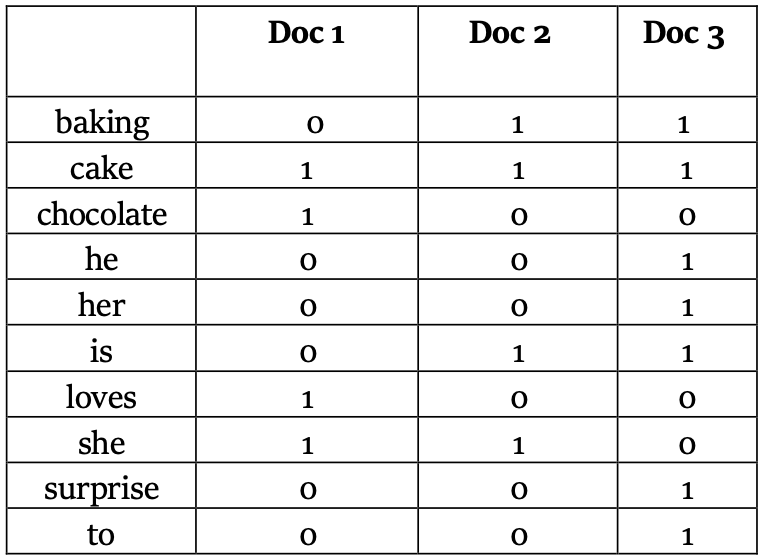
\includegraphics[scale=0.5]{static/table_bow.png}
        \caption{\label{fig:table_bow} Bag-of-words Sparse Matrix \cite{Buddhadev2025}}
    \end{subfigure}
    \begin{subfigure}{0.5\textwidth}
        \centering
        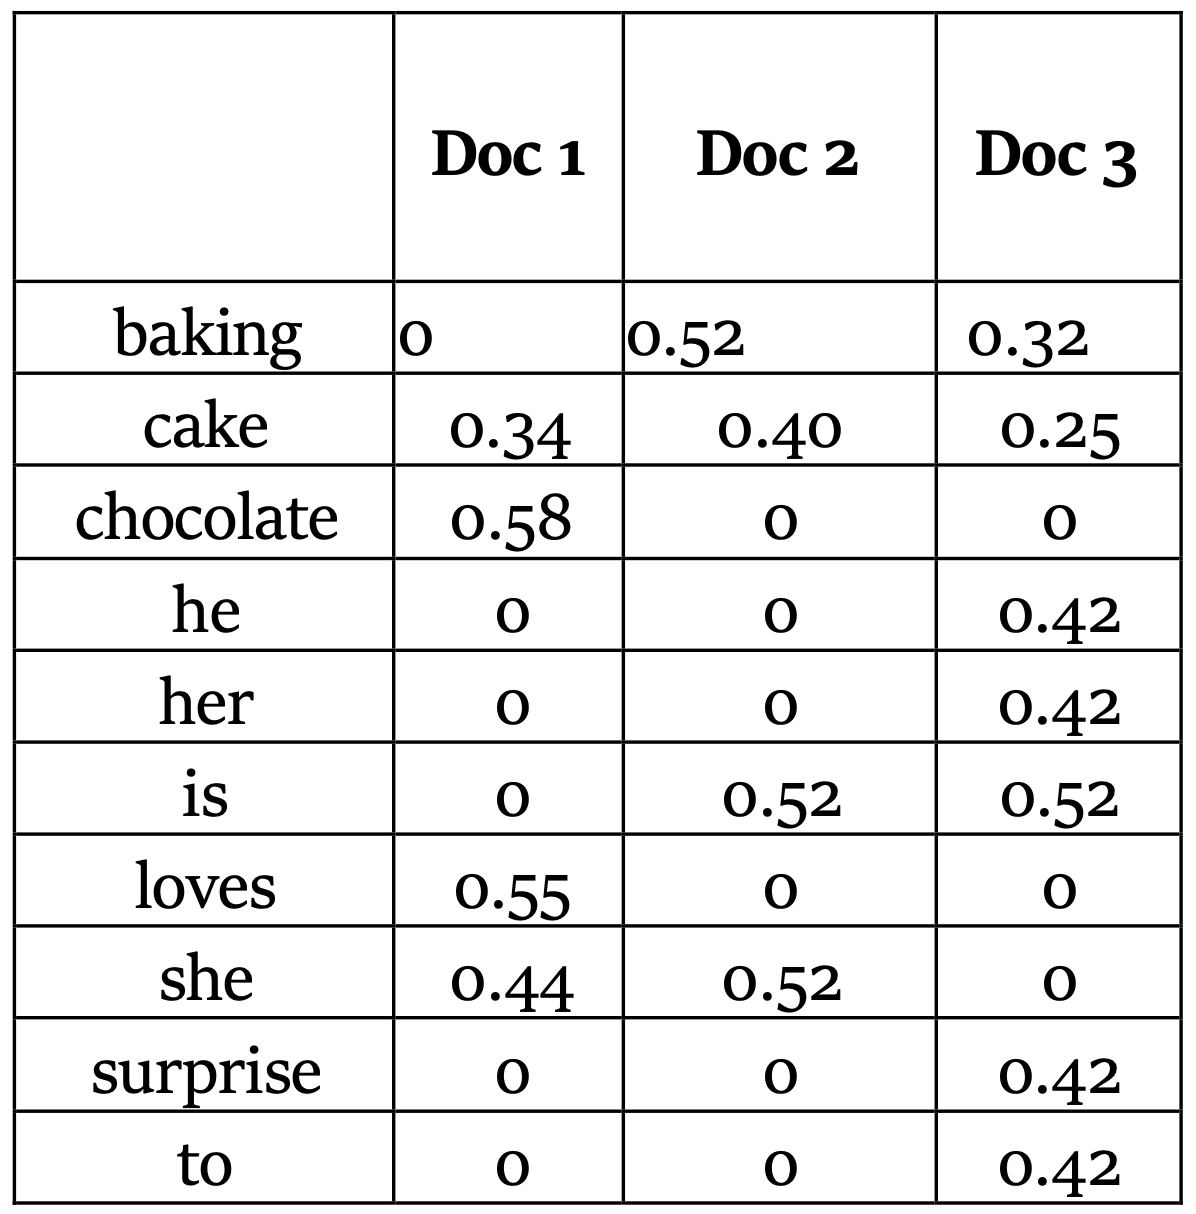
\includegraphics[scale=0.25]{static/table_tf-idf.png}
        \caption{\label{fig:table_tf-idf} TF-IDF Sparse Matrix \cite{Buddhadev2025}}
    \end{subfigure}
    
    \caption{Vergleich der Sparse Matrizen}
    \label{fig:vlg_sparse_matrizen}
\end{figure}

In Abbildung \ref{fig:vlg_sparse_matrizen} wurden den beiden Matrizen jeweils die drei Dokumente:

\begin{itemize}
    \item Doc1 - She loves chocolate cake
    \item Doc2 - She is baking a cake
    \item Doc3 - He is baking a cake to surprise her
\end{itemize}

hinzugefügt. In der Matrix \ref{fig:table_bow} werden in jeder Zelle in welcher das Dokument das entsprechende Wort beinhaltet eine 1 gesetzt.
In \ref{fig:table_tf-idf} wird statt einer 1 eine Gewichtung über die Häufigkeit der Wörter in allen Dokumenten hinweg erstellt und eingetragen.
Sie bewertet die Wichtigkeit eines Wortes in einem Dokument relativ zur gesamten Sammlung von Dokumenten. Dabei wird die Termfrequenz (TF) mit der 
invertierten Dokumentfrequenz (IDF) multipliziert. Je höher der resultierende Wert, desto relevanter ist das Wort für das jeweilige Dokument. 
Die Formel lautet:

\begin{equation}
    \text{tfidf}(t, d, D) = \text{tf}(t, d) \cdot \text{idf}(t, D)
\end{equation}

Dabei ist \( t \) das Wort, \( d \) das Dokument und \( D \) die gesamte Dokumentensammlung \cite{aslam2022}.

Die TF misst, wie häufig ein bestimmter Begriff \( t \) in einem Dokument \( d \) vorkommt. 
Sie beschreibt die lokale Bedeutung eines Wortes innerhalb des Dokuments.

\begin{equation}
\text{tf}(t, d) = \frac{\text{Anzahl der Vorkommen von } t \text{ in } d}{\text{Gesamtanzahl der Wörter in } d}
\end{equation}

Die IDF bewertet, wie selten ein Begriff \( t \) in der gesamten Dokumentensammlung \( D \) ist. 
Je seltener ein Begriff in vielen Dokumenten vorkommt, desto höher ist sein IDF-Wert.

\begin{equation}
    \text{idf}(t, D) = \log \left( \frac{N}{\text{df}(t)} \right)
\end{equation}

Dabei ist \( N \) die Gesamtanzahl der Dokumente in der Matrix und \( \text{df}(t) \) die Anzahl der Dokumente, 
in denen der Begriff \( t \) vorkommt \cite{qaiser2018}.

Die in \cite{Domenico2016} beschriebene Relevance Frequency (RF) ist eine überwachte Gewichtungsform der IDF-Komponente im TF-IDF, die nicht nur zählt, 
in wie vielen Dokumenten ein Begriff vorkommt, sondern berücksichtigt, in welchen Klassen der Begriff besonders häufig oder exklusiv ist.
Die Formel lautet:

\begin{equation}
    \text{rf}(t) = \log\left(2 + \frac{P(t)}{\max(1, N(t))} \right)
\end{equation}

Mit \( P(t) \) für die Anzahl der relevanten Dokumente (z.\,B. positive Klasse), in denen der Term \( t \)
und \( N(t) \) für die Anzahl der irrelevanten Dokumente (z.\,B. negative Klasse), in denen der Term \( t \) vorkommt.

Während klassisches IDF ein Wort umso höher gewichtet, je seltener es allgemein in der Gesamtmatrix ist,
gewichtet RF hingegen ein Wort umso höher, je stärker es mit einer bestimmten Zielklasse assoziiert ist.
Dadurch hebt RF Begriffe hervor, die klassenunterscheidend sind was beim Arbeiten mit überwachten Modellen relevant ist.

In der IF-IDF wird für IDF wird nun also RF eingesetzt und es ergibt sich folgende Formel:

\begin{equation}
    \text{tfidf}(t, d) = \frac{\text{Anzahl der Vorkommen von } t \text{ in } d}{\text{Gesamtanzahl der Wörter in } d} \cdot \log\left(2 + \frac{P(t)}{\max(1, N(t))} \right)
\end{equation}

\begin{itemize}
    \item Mit dem Wort \( t \) und dem Dokument \( d \) 
    \item \( P(t) \) für die Anzahl der relevanten Dokumente (z.\,B. positive Klasse), in denen der Term \( t \) vorkommt
    \item \( N(t) \) für die Anzahl der irrelevanten Dokumente (z.\,B. negative Klasse), in denen der Term \( t \) vorkommt
\end{itemize}

\subsubsection{Vergleich Bag-of-words und TF-IDF}

\begin{table}[!ht]
    \centering
        \begin{tabular}{|p{6.6cm}|p{6.6cm}|}
            \hline
            \textbf{Bag-of-Words (BoW)} & \textbf{TF-IDF} \\
            \hline
            Einfache Implementierung \cite{cichosz2018forum} & Berücksichtigt Wortwichtigkeit in gesamter Matrix  \cite{elov2023uzbek} \\
            \hline
            Keine Gewichtung — häufige Wörter dominieren & Seltener, aber informativer Inhalt wird stärker gewichtet \cite{das2023tfidf} \\
            \hline
            Hohe Dimensionalität in Sparse Matrix (jedes Wort bekommt eine separate Dimension) \cite{ibm_bow} & Gleiches Problem, aber mit informativeren Werten \cite{alzami2020tfidf} \\
            \hline
            Ignoriert Wortreihenfolge und Kontext \cite{umar2022sentiment} & Gleiches Grundproblem, aber geringfügig bessere Performance \cite{parmar2024stacking} \\
            \hline
            Nützlich für einfache Klassifikatoren & Bessere Klassifikationsergebnisse in Kombination mit SVM oder Logistic Regression \cite{iyer2024sentiment} \\
            \hline
        \end{tabular}
    \caption{Vergleich der Vor- und Nachteile von BoW und TF-IDF}
    \label{tab:vergleich}
\end{table}

Aus Tabelle \ref{tab:vergleich} zu erkennen ist, dass TF-IDF in vielen Anwendungen leistungsfähiger ist als BoW. Insbesondere bei Texten mit hohem Vokabularumfang.

\subsubsection{Hashing Vectorizer}

Ein Hashing Vectorizer ist eine Methode zur Umwandlung von Text in numerische Merkmalsvektoren, ohne dass ein Vokabular explizit 
erstellt oder gespeichert wird. Stattdessen wird eine Hash-Funktion verwendet, um jedes Wort auf einen Index im Feature-Vektor abzubilden \cite{Buddhadev2025}.

In Abbildung \ref{fig:vgl_bow_tfidf_hashing} wird der Vergleich zwischen Machine-Learning-Modellen unter Verwendung von BoW-, TF-IDF- und
Hashing-Features gezeigt. Die y-Achse präsentiert den F1-Score, also die Precision und Recall-Werte der jeweiligen Modelle.
Das Random-Forest-Modell (RF) zeigt eine schwache Leistung bei der Verwendung von Hashing, während die linearen Modelle 
(z.B. SVM (Support Vector Machine) und LR (Logistische Regression)) ihre F1-Werte mit Hashing-Features verbessern konnten. 

Die Verbesserung ist aber nur minimal. Der F1-Score bei SVM ist ohne Hashing bei 0.89 und nach bei 0.90. 
Bei LR steigt der Wert auch von 0.87 und 0.88.

\begin{figure}[htbp]
    \begin{center}
        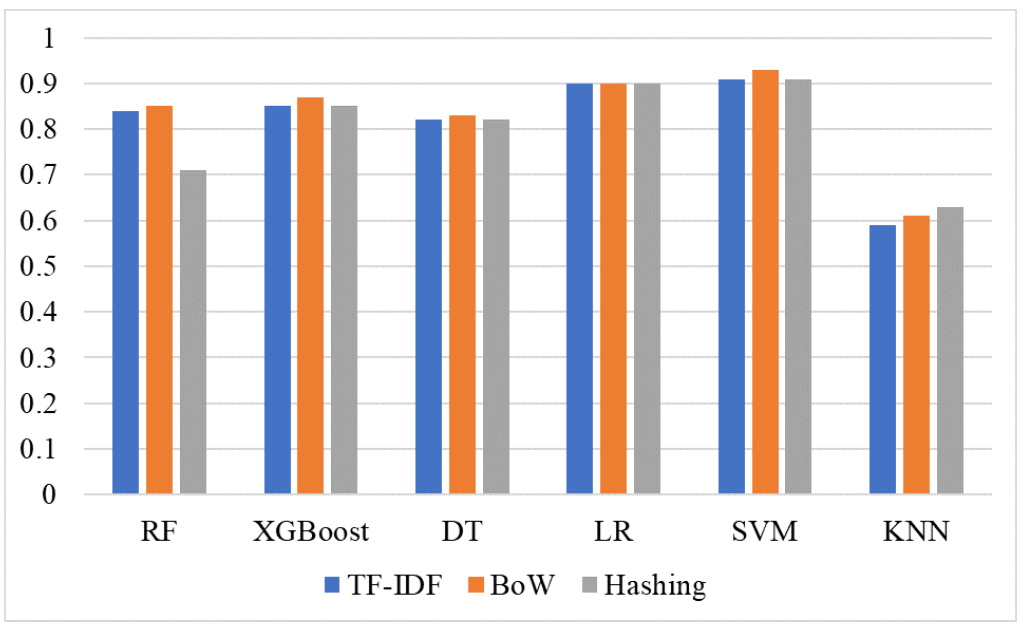
\includegraphics[scale=0.5]{static/bow_vs_tfidf_vs_hashing.png}
        \caption{\label{fig:vgl_bow_tfidf_hashing} Vergleich verschiedener Modelle mit BoW, TF-IDF und Hashing \cite{aslam2022}}
    \end{center}
\end{figure}

\subsection{Machine Learning Modelle}
\label{sec:ml_modelle}

\subsubsection{Naive-Bayes}

Der Naive-Bayes-Algorithmus ist ein einfacher, aber leistungsfähiger Klassifikator, der auf dem Satz von Bayes basiert. 
Er wird häufig in Bereichen wie Textklassifikation, Spam-Erkennung und Sentiment-Analyse eingesetzt \cite{zhang2004}.

Der Klassifikator nutzt den Satz von Bayes zur Berechnung der Wahrscheinlichkeit einer Klasse \( C \) gegeben eine Merkmalsmenge \( X \):

\begin{equation}
    P(C \mid X) = \frac{P(X \mid C) \cdot P(C)}{P(X)}
\end{equation}

Dabei ist:

\begin{itemize}
  \item \textbf{\( P(C \mid X) \)} – \emph{Posterior}: Die Wahrscheinlichkeit für die Klasse \( C \), nachdem die Daten \( X \) beobachtet wurden.
  \item \textbf{\( P(X \mid C) \)} – \emph{Likelihood}: Die Wahrscheinlichkeit, die Daten \( X \) zu sehen, wenn sie zur Klasse \( C \) gehören.
  \item \textbf{\( P(C) \)} – \emph{Prior}: Die ursprüngliche Wahrscheinlichkeit der Klasse \( C \), ohne Kenntnis über die Daten.
  \item \textbf{\( P(X) \)} – \emph{Evidenz}: Die Gesamtwahrscheinlichkeit, die Daten \( X \) zu beobachten (über alle Klassen hinweg).
\end{itemize}

Die zentrale Annahme des Naive-Bayes-Klassifikators ist die bedingte Unabhängigkeit der Merkmale:

\begin{equation}
    P(X \mid C) = \prod_{i=1}^{n} P(x_i \mid C)
\end{equation}

Dies vereinfacht die Berechnung erheblich, da nur die Wahrscheinlichkeiten einzelner Merkmale betrachtet werden müssen \cite{webb2010naive}.

\subsubsection{Decision Tree}

Ein Decision Tree (Entscheidungsbaum) ist ein Algorithmus für Klassifikation und Vorhersage. 
Er basiert auf einer baumartigen Struktur, bei der jeder Knoten bzw. Ast ein Merkmal aus einem Datensatz repräsentiert. 
Diese Struktur ermöglicht es, schrittweise Entscheidungen zu treffen, die schließlich zu einer Klassenzuordnung an einem Blattknoten führen \cite{10.3389/frai.2023.1124553}.

Der Baum wird durch Auswahl von Merkmalen aufgebaut, die die Daten am besten aufspalten. 
Dieses Auswahlkriterium basiert auf dem Konzept der \textbf{Entropie} und dem daraus abgeleiteten \textbf{Informationsgewinn}. 
Ziel ist es, bei jeder Entscheidung im Baum das Merkmal auszuwählen, das die größte Reduktion an Unsicherheit bietet.

Die Entropie misst die Unreinheit oder Unbestimmtheit eines Datensatzes. Sie ist dann maximal, 
wenn alle Klassen gleichverteilt sind, und minimal (d.h. null), wenn alle Daten zur selben Klasse gehören. 
Die Entropie \( E(S) \) eines Datensatzes \( S \) wird wie folgt berechnet:

\begin{equation}
    E(S) = - \sum_{i=1}^{c} p_i \log_2 p_i
\end{equation}

Dabei ist:
\begin{itemize}
  \item \( c \) die Anzahl der Klassen,
  \item \( p_i \) der Anteil der Klasse \( i \) im Datensatz \( S \).
\end{itemize}

Der Informationsgewinn misst die Reduktion der Entropie, die durch das Aufteilen eines Datensatzes mittels eines bestimmten Merkmals erzielt wird. Je größer der Informationsgewinn, desto besser ist das Merkmal für die Aufspaltung geeignet. Eine alternative Formel für den Informationsgewinn $IG(E)$ lautet:

\begin{equation}
    IG(E) = 1 - \sum_{i=1}^{c} p_i^2
\end{equation}

Über einen Hyperparameter kann die maximale Tiefe des Baumes festlegt werden. 
Eine zu große Tiefe kann zu Overfitting führen, da der Baum zu sehr an die Trainingsdaten angepasst wird \cite{aslam2022}.


\subsubsection{Random Forest}

Ein Random Forest besteht aus einer großen Anzahl von Entscheidungsbäumen. 
Jeder Baum wird auf einem zufällig gezogenen Teildatensatz trainiert (Bagging). 
Bei der Bildung jedes Knotens (Split) wird eine zufällige Teilmenge von Merkmalen berücksichtigt. 
Die finale Klassifikation ergibt sich durch Mehrheitsentscheidung aller Bäume (Ensemble Voting) \cite{elchami2025}.

Die Bedeutung eines Merkmals \( i \) im Random Forest ergibt sich aus der durchschnittlichen normierten Bedeutung 
dieses Merkmals über alle Entscheidungsbäume hinweg. Diese kann mathematisch wie folgt dargestellt werden:

\begin{equation}
    RFf_i = \frac{\sum_{j \in \text{all trees}} normf_{ij}}{T}
\end{equation}

Dabei ist:
\begin{itemize}
    \item \( RFf_i \) die Gesamtrelevanz der Klasse \( i \) im gesamten Wald,
    \item \( normf_{ij} \) die normierte Wichtigkeit des Merkmals \( i \) im Baum \( j \),
    \item \( T \) die Gesamtanzahl der Entscheidungsbäume \cite{aslam2022}.
\end{itemize}

Wichtige Hyperparameter sind hier:
\begin{itemize}
    \item \texttt{n\_estimators}: Anzahl der Entscheidungsbäume im Wald.
    \item \texttt{max\_depth}: Maximale Tiefe der Bäume.
    \item \texttt{max\_features}: Anzahl der Merkmale, die für einen Split berücksichtigt werden.
    \item \texttt{bootstrap}: Gibt an, ob Stichproben mit Zurücklegen gezogen werden.
\end{itemize}

Im Vergleich zu Decision Trees ist Random Forest robuster gegenüber Overfitting und bringt durch das Ensemble Voting eine 
höhere Genauigkeit \cite{al-tarawneh2025}.

\subsubsection{Support Vector Machines}

Support Vector Machines (SVMs) sind überwachte Lernalgorithmen, die besonders effektiv für Klassifikationsaufgaben sind. 
Sie finden breite Anwendung in Bereichen wie Bioinformatik, Textklassifikation und 
insbesondere in der Erkennung von Fake News. 
Das Ziel einer SVM ist es, eine Trennlinie --- oder in höherdimensionalen Räumen ein Trenn-Hyperplane --- zu finden, 
das Datenpunkte verschiedener Klassen mit maximalem Abstand (Margin) voneinander trennt  \cite{Noble:2006aa, Buddhadev2025, sabir2025, jakkula2006tutorial}.

\textbf{1. Ziel: Eine Trennebene finden}
Eine SVM sucht eine Gerade (in 2D), Ebene (in 3D) oder Hyperplane, die die Klassen voneinander trennt:
\begin{equation}
w^T x + b = 0
\end{equation}

\textbf{2. Bedingung für korrekte Trennung}
Für jeden Punkt \( x_i \) mit zugehörigem Label \( y_i \in \{-1, +1\} \) gilt:
\begin{equation}
y_i(w^T x_i + b) \geq 1
\end{equation}

\begin{figure}[htbp]
    \begin{center}
        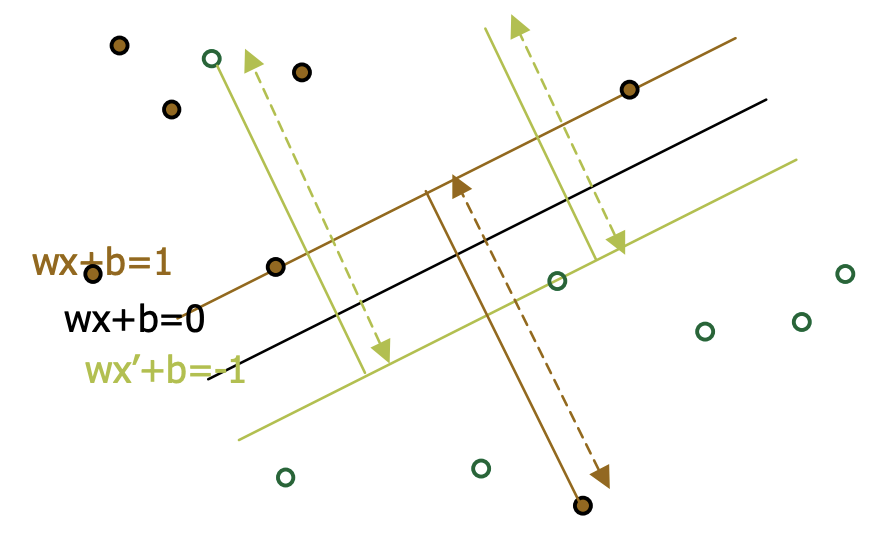
\includegraphics[scale=0.5]{static/fig_hyperplanes.png}
        \caption{\label{fig:hyperplanes} Darstellung von Hyperplanes \cite{jakkula2006tutorial}}
    \end{center}
\end{figure}

\textbf{3. Margin maximieren}
Der Margin ist der Abstand der nächsten Punkte beider Klassen zur Trennebene:
\begin{equation}
M = \frac{2}{\|w\|}
\end{equation}

Daher wird zur Maximierung des Margins folgende Zielfunktion minimiert:
\begin{equation}
\min_{w, b} \quad \frac{1}{2} \|w\|^2
\quad \text{mit} \quad y_i(w^T x_i + b) \geq 1
\end{equation}

\textbf{4. Fehler zulassen – Soft Margin}

Bei nicht perfekt trennbaren Daten werden sogenannte Slack-Variablen \( \xi_i \) eingeführt:
\begin{equation}
y_i(w^T x_i + b) \geq 1 - \xi_i, \quad \xi_i \geq 0
\end{equation}

Ziel ist es, Fehler klein zu halten, gleichzeitig aber den Margin möglichst groß:
\begin{equation}
\min \left( \frac{1}{2} \|w\|^2 + C \sum \xi_i \right)
\end{equation}

\textbf{5. Nichtlineare Trennung – Kernel-Trick}

Bei komplexen Datensätzen wird das Problem durch eine Funktion \( \phi \) in höhere Dimensionen überführt, ohne sie explizit zu berechnen \cite{jakkula2006tutorial}:
\begin{equation}
K(x_i, x_j) = \phi(x_i)^T \phi(x_j) 
\end{equation}

Gängige Kernel-Funktionen:
\begin{itemize}
  \item Linearkernel: \( K(x, x') = x^T x' \)
  \item Polynomial: \( K(x, x') = (x^T x' + 1)^d \)
  \item Radial Basis Function (RBF): \( K(x, x') = \exp(-\gamma \|x - x'\|^2) \) \cite{jakkula2006tutorial}
\end{itemize}
\cite{Noble:2006aa} zeigt, dass durch geeignete Wahl eines Kernels auch komplex strukturierte Daten erfolgreich klassifiziert werden können.

\textbf{Es ergibt sich folgender Ablauf:}

\begin{enumerate}
  \item Definiere Trennebene: \( w^T x + b = 0 \)
  \item Erzwinge korrekte Trennung: \( y_i(w^T x_i + b) \geq 1 \)
  \item Maximiere Margin: \( \min \frac{1}{2} \|w\|^2 \)
  \item Erlaube kleine Fehler: \( \min \frac{1}{2} \|w\|^2 + C \sum \xi_i \)
  \item Wende ggf. Kernel an: \( K(x_i, x_j) = \phi(x_i)^T \phi(x_j) \)
\end{enumerate}

\textbf{Vorteile von SVMs sind:}

\begin{itemize}
    \item \textbf{Robustheit gegenüber Overfitting}, insbesondere bei hoher Dimensionalität und geringem Datensatz \cite{Noble:2006aa}.
    \item \textbf{Gute Generalisierungsfähigkeit} durch Maximierung des Margins.
    \item \textbf{Effizient in der Praxis}: Für viele reale Probleme sind SVMs konkurrenzfähig gegenüber tieferen Netzwerken, (z.B. in Fake-News-Klassifikationen) \cite{Buddhadev2025, sabir2025}.
    \item \textbf{Flexibilität durch Kernel-Funktionen}, womit verschiedene Datentypen (z.B. Vektoren, Strings, Graphen) verarbeitet werden können.
\end{itemize}

\subsubsection{Logistische Regression}

Die logistische Regression (LR) ist ein weit verbreitetes Verfahren des überwachten maschinellen Lernens zur Klassifikation binärer und 
multiklassiger Zielvariablen. Sie wird eingesetzt, um die Wahrscheinlichkeit zu berechnen, mit der eine Beobachtung zu einer 
bestimmten Klasse gehört \cite{elchami2025, aslam2022, SUDHAKAR2024101028}. Im Gegensatz zur linearen Regression verwendet LR eine Aktivierungsfunktion, 
typischerweise die Sigmoidfunktion, um Ausgaben zwischen 0 und 1 abzubilden. Diese Werte stellen Wahrscheinlichkeiten dar und werden zur 
Vorhersage diskreter Zielwerte genutzt \cite{aslam2022}. Die Tabelle \ref{tab:linkfunktionen} zeigt die Aktivierungsfunktionen, mit deren entsprechend
benötigten Zielvariablen.

\begin{table}[ht]
    \centering
        \begin{tabular}{|p{4.4cm}|p{4.4cm}|p{4.4cm}|}
        \hline
        \textbf{Typ} & \textbf{Aktivierungsfunktion} & \textbf{Typ der Zielvariable}\\
        \hline
        Binäre logistische Regression & Logit (Sigmoid): $\frac{1}{1 + e^{-z}}$ & Binär (0/1) \\
        \hline
        Multinomiale logistische Regression & Softmax: $\frac{e^{z_k}}{\sum_j e^{z_j}}$ & Kategorisch (mehrere Klassen) \\
        \hline
        Ordinale logistische Regression & Cumulative Logit, Probit, Cloglog & Geordnete Klassen \\
        \hline
        Probit-Modell & $\Phi(z)$ (Normalverteilung) & Binär (0/1), robust gegen Ausreißer \\
        \hline
        \end{tabular}
\caption{Übersicht von Aktivierungsfunktion in der logistischen Regression \cite{jurafsky2023, hastie2009, agresti2018cda}}
\label{tab:linkfunktionen}
\end{table}

Das Ziel der logistischen Regression ist es, eine Funktion zu finden, die die Wahrscheinlichkeit \( P \) berechnet, 
dass ein Eingabewert \( X \) zur Klasse \( y = 1 \) gehört. Dies geschieht zum Beispiel mittels der Sigmoidfunktion \cite{jurafsky2023}:

\begin{equation}
    P = \frac{1}{1 + e^{-(a + bX)}}
\end{equation}

Dabei sind:
\begin{itemize}
  \item \( P \): Wahrscheinlichkeit für Klasse 1 (Wert zwischen 0 und 1)
  \item \( X \): Eingabewert (Merkmalsvariable)
  \item \( b \): Gewicht des Merkmals
  \item \( a \): \textbf{Bias} oder \textbf{Intercept}, also der Schnittpunkt mit der y-Achse, verschiebt die Entscheidungsgrenze. 
  Ohne Bias würde die Entscheidungsgrenze immer durch den Ursprung laufen, was in der Praxis selten sinnvoll ist \cite{geron2019}.
\end{itemize}

In \cite{elchami2025} wurde der Intercept explizit deaktiviert, wodurch sich die Gleichung zu \( P = 1 / (1 + e^{-bX}) \) vereinfacht.

\textbf{Vorteile der logistischen Regression:}
\begin{itemize}
  \item \textbf{Einfachheit und Interpretierbarkeit}: LR-Modelle sind leicht verständlich und liefern direkt interpretierbare Wahrscheinlichkeiten \cite{aslam2022}.
  \item \textbf{Effizienz}: Sie sind schnell trainierbar und benötigen relativ geringe Rechenleistung \cite{SUDHAKAR2024101028}.
  \item \textbf{Flexibilität}: LR lässt sich für binäre, multinomiale und ordinale Klassifikationsprobleme erweitern \cite{SUDHAKAR2024101028}.
  \item \textbf{Breite Anwendbarkeit}: Sie wird in zahlreichen Bereichen eingesetzt, von der Medizin bis zur Textklassifikation \cite{aslam2022, elchami2025}.
\end{itemize}

\subsubsection{K-Nearest Neighbor}

Der K-Nearest Neighbor (KNN) Algorithmus ist ein überwachter Lernalgorithmus, der unter anderem für Klassifikationsprobleme eingesetzt wird. 
Er gehört zur Gruppe der sogenannten lazy learners, da kein expliziter Trainingsprozess stattfindet. 
Stattdessen wird der Trainingsdatensatz während der Vorhersage verwendet \cite{Verma:2024aa}.

KNN klassifiziert neue Instanzen auf Basis ihrer Ähnlichkeit mit bereits bekannten Beispielen. 
Dazu berechnet es die Distanz zwischen dem Testpunkt und allen Trainingspunkten. 
Anschließend werden die \( K \) ähnlichsten Punkte ausgewählt und die Vorhersage erfolgt bei Klassifikation durch 
Mehrheitsentscheidung \cite{aslam2022}.

Die Distanzmessung erfolgt in der Regel über die \textbf{euklidische Distanz}, mit der gemessen wird, 
wie weit zwei Punkte im Merkmalsraum voneinander entfernt sind. Die Formel lautet:

\begin{equation}
    E_d = \sqrt{ \sum_{i=1}^{k} (x_i - y_i)^2 }
\end{equation}

Dabei sind:
\begin{itemize}
    \item \( x_i \): der \( i \)-te Wert des zu klassifizierenden Punkts
    \item \( y_i \): der entsprechende \( i \)-te Wert eines bekannten Trainingspunkts
    \item \( k \): die Anzahl der Merkmale (Dimensionen), z.B. bei Textdaten die Länge des Vektors
\end{itemize}

Je kleiner der Wert \( E_d \), desto ähnlicher sind sich die beiden Punkte.

Der KNN-Algorithmus verwendet mehrere wichtige Hyperparameter:

\begin{enumerate}
    \item \textbf{n\_neighbors}: Gibt an, wie viele der nächsten Trainingspunkte zur Klassifikation berücksichtigt werden. 
    Der Wert (oft als \( K \) bezeichnet) sollte basierend auf den Eigenschaften des Datensatzes gewählt werden \cite{Verma:2024aa, aslam2022}.

    \item \textbf{weights}: Bestimmt, ob allen Nachbarn das gleiche Gewicht gegeben wird oder ob näher gelegene Punkte stärker 
    gewichtet werden \cite{knnparams2024}.

    \item \textbf{metric}: Die Distanzmetrik zur Berechnung der Ähnlichkeit. Standardmäßig wird die euklidische Distanz verwendet, 
    möglich sind aber auch Manhattan, Minkowski oder andere Metriken \cite{aslam2022}
\end{enumerate}

Auch wenn KNN einfach und intuitiv zu implementieren ist und keinen Trainingsprozess benötigt, zeigt Abbildung \ref{fig:nlp_models}, 
dass es im Vergleich mit Naive Bayes (NB), logistischer Regression (LG) und Support Vector Machines (SVM) ein vergleichsweise ineffektives Model 
für NLP ist.

\begin{figure}[htbp]
    \begin{center}
        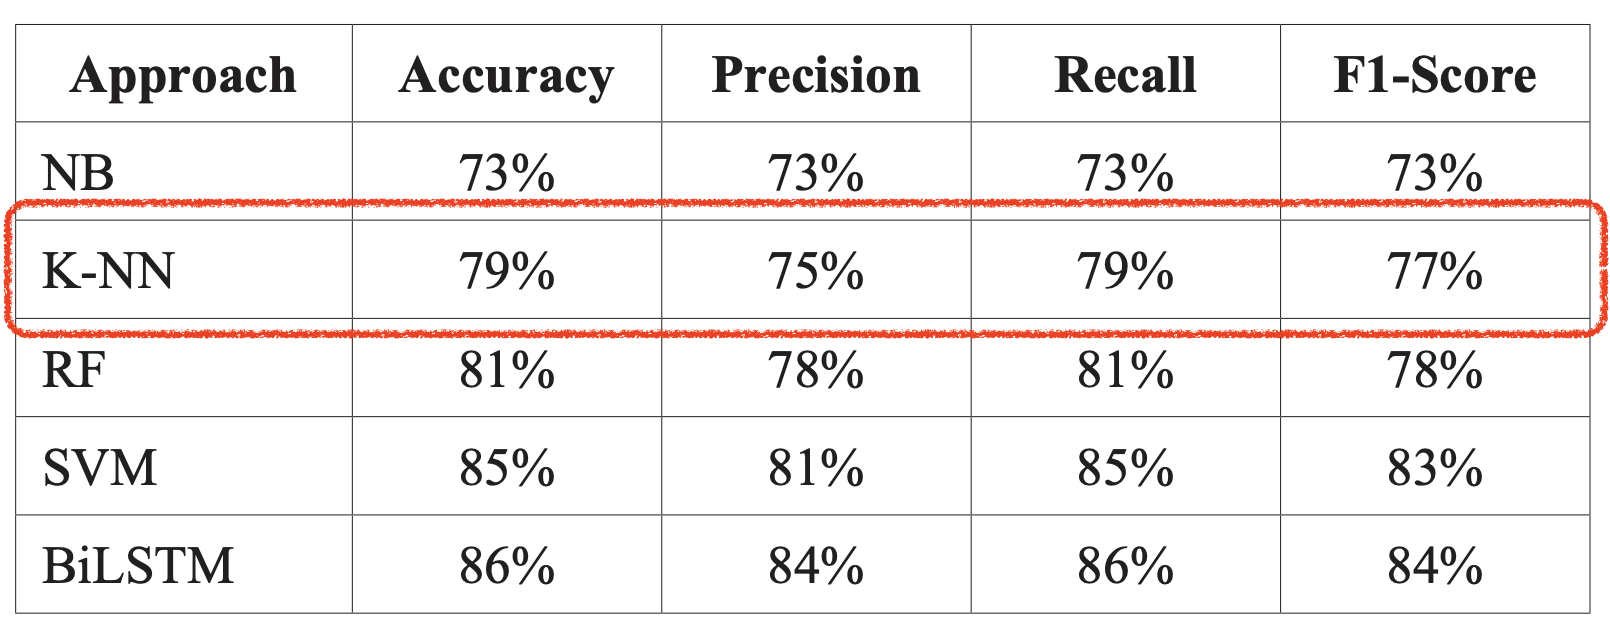
\includegraphics[scale=0.4]{static/vgl_svm_knn_etc.png}
        \caption{\label{fig:nlp_models} Auswertung verschiedener NLP Algorithmen \cite{prom2024}}
    \end{center}
\end{figure}

Hier wurde KNN zur Klassifikation in einem Stimmungserkennungs-System für die Amtssprache Kambodschas eingesetzt. 
Dabei diente KNN dem Vergleich mit anderen Ansätzen wie SVM und wurde insbesondere hinsichtlich seiner Leistung bei der 
Klassifikation von Textdaten bewertet, bei denen die Reihenfolge, der Zeitpunkt oder der Verlauf über die Zeit eine wichtige Rolle 
für die Interpretation und Analyse spielt.

\subsubsection{XGBoost}

eXtreme Gradient Boosting (XGBoost) ist eine Implementierung von Gradient Boosting Decision Trees (GBDT).
Beim XGBoost wird das Modell durch die Addition mehrerer Entscheidungsbäume aufgebaut, welche als
schwache Lernalgorithmen (base learners) fungieren. 
Anders als bei Random Forests, bei denen Bäume unabhängig voneinander trainiert und aggregiert werden, 
lernen die Bäume in XGBoost aufeinander aufbauend (siehe Abbildung \ref{fig:xgboost}). Die Vorhersage für ein Beispiel ergibt sich aus der Summe der 
Ausgaben aller zuvor gelernten Bäume. Dadurch entsteht ein starkes Modell, das schrittweise durch Fehlerkorrektur 
verbessert wird \cite{petrovic2024,chen2016xgboost,aslam2022}.

\begin{figure}[htbp]
    \begin{center}
        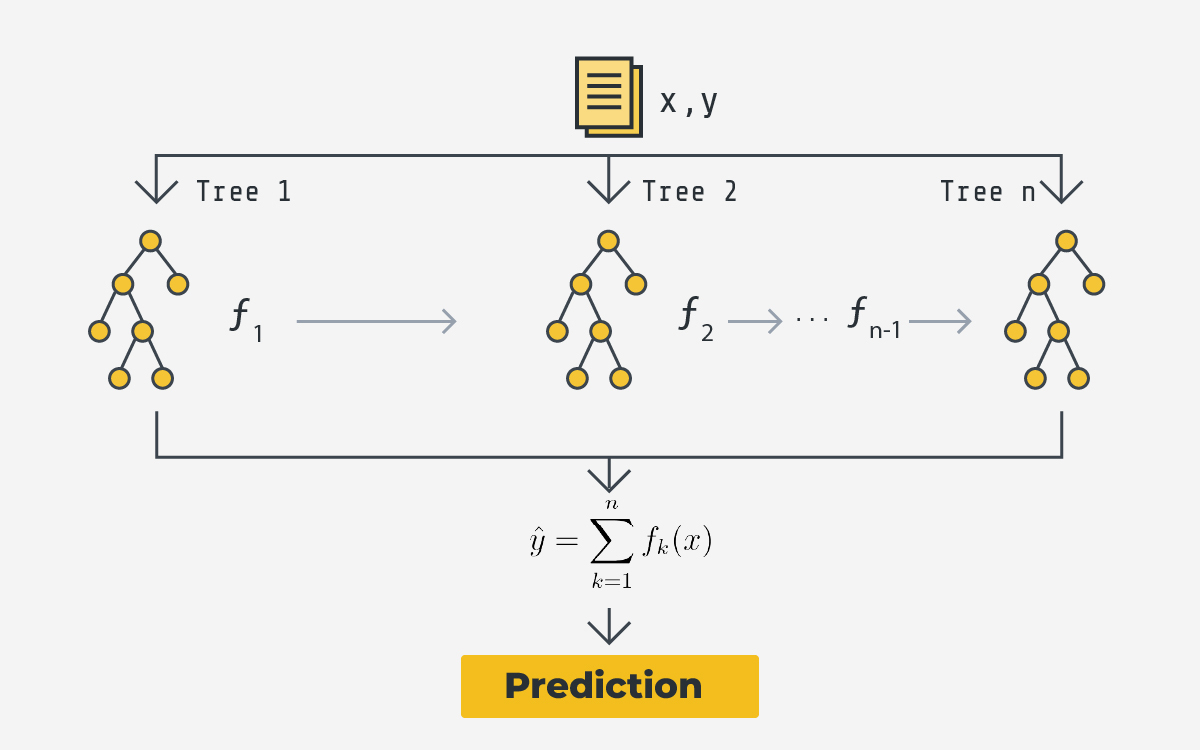
\includegraphics[scale=0.25]{static/xgboost-pipeline.jpg}
        \caption[XGBoost]{\label{fig:xgboost} XGBoost\footnotemark}
    \end{center}
\end{figure}
\footnotetext{\url{https://flower.ai/blog/2023-11-29-federated-xgboost-with-bagging-aggregation/}}

Ein zentraler Vorteil von XGBoost ist die integrierte Regularisierung, mit der das Modell Overfitting vermeiden kann. 
Dabei werden zwei Arten von Regularisierung eingesetzt:

\begin{itemize}
    \item \textbf{L1-Regularisierung}: Bestraft große Gewichtswerte, indem sie einige Gewichte auf Null setzt. 
        Dadurch hilft sie, unwichtige Merkmale automatisch zu entfernen.
    \item \textbf{L2-Regularisierung}: Bestraft extreme Gewichtswerte, ohne sie komplett zu eliminieren. 
        Dies führt zu stabileren Modellen mit kleinen, gleichmäßigen Gewichten.
\end{itemize}

Beide Regularisierungen sind in die sogenannte Ziel- oder Kostenfunktion eingebettet, die das Modell bei jedem Trainingsschritt minimiert. 

In Anwendungen der natürlichen Sprachverarbeitung (NLP) hilft diese Kombination, besonders bei großen Textmerkmalräumen (z.B. TF-IDF), 
relevante Merkmale herauszufiltern und gleichzeitig stabile Modelle zu trainieren\cite{chen2016xgboost}.

\subsubsection{LightGBM}

Das von \cite{ke2017} entwickelte Modell \textit{Light Gradient-Boosting Machine (LightGBM)} ist eine hocheffiziente Implementierung eines GBDT. 
In Bezug auf dieses Modell wurden zwei zentrale Innovationen eingeführt, um das Training bei großen und hochdimensionalen Datensätzen zu beschleunigen, 
ohne die Modellgenauigkeit zu beeinträchtigen:

\paragraph{Gradient-based One-Side Sampling (GOSS)} reduziert den Rechenaufwand von GBDT, indem es nur einen Teil der Dateninstanzen für die Berechnung 
der Informationsgewinne nutzt. Instanzen mit großen Gradienten (hohem Fehler) werden vollständig beibehalten, während aus den Instanzen mit kleinen 
Gradienten eine Stichprobe gezogen wird. Ein Gewichtungsschritt stellt sicher, dass die Verteilung der Daten korrekt bleibt. Dies führt zu einer
deutlich schnelleren Trainingszeit bei nahezu gleichbleibender Genauigkeit.

\paragraph{Exclusive Feature Bundling (EFB)} adressiert das Problem vieler hochdimensionaler Datensätze, in denen viele Merkmale nur selten 
(sogenannte \textit{sparse} Features) oder nie gleichzeitig (\textit{mutually exclusive}) aktiv sind. 
\textit{Sparse} bedeutet, dass die meisten Werte in einem Merkmal Null sind, während \textit{mutually exclusive} bedeutet, dass bestimmte Merkmale sich 
gegenseitig ausschließen – also nicht gleichzeitig einen von Null verschiedenen Wert annehmen. 
EFB fasst solche Merkmale zu sogenannten Bundles zusammen, wodurch sich die Anzahl der zu verarbeitenden Merkmale stark reduziert. 
Das Bündelungsproblem wird als Graphfärbungsproblem modelliert und mit einem Greedy-Algorithmus angenähert.
Dadurch wird der Histogrammaufbau effizienter und das Training insgesamt beschleunigt.

Sowohl \cite{ke2017} als auch \cite{hu2020} zeigen, dass LightGBM gegenüber XGBoost effizienter trainiert, eine bessere Vorhersage gibt, weniger
Merkmale benötigt und Kktegorische Daten einfacher bearbeiten kann, dementsprechend also auch kein One-Hot-Encoding benötigt.

\subsection{Metriken}

Zur Auswertung der überwachten Modelle werden Metriken genutzt. Die Auswahl der richtigen Metriken hängt von der gewünschten Zielsetzung ab.
Diese kann zum Beispiel binäre, bzw. multi-Klassen Klassifikation oder Regression sein.

Fake News Erkennung ist eine binäre Klassifizierung (Der Artikel ist entweder 'wahr' oder 'falsch').

Dabei ergeben sich vier mögliche Ausgänge bei der Modellvorhersage:
\begin{itemize}
    \item True Positive (TP) - Das Modell hat die positive Klasse vorhergesagt. 
        
    (Der Artikel, der kein Fake ist, wird als 'wahr' gedeutet)
    \item True Negative (TN) - Das Modell hat die negative Klasse richtig vorhergesagt.
        
    (Der Artikel, der Fake ist, wird als 'falsch' gedeutet)
    \item Falsch positiv (FP) - Das Modell hat die positive Klasse falsch vorhergesagt. 
        
    (Der Artikel, der kein Fake ist, wird als 'falsch' gedeutet)
    \item Falsches Negativ (FN) - Dein Modell hat die negative Klasse falsch vorhergesagt. 
        
    (Der Artikel, der kein Fake ist, wird als 'wahr' gedeutet)
\end{itemize}

Diese vier Werte werden in einer sogenannten Konfusionsmatrix  (siehe Abbildung \ref{fig:confusion_matrix}) zusammengefasst
aus der verschiedene Bewertungsmetriken abgeleitet werden können.

\begin{figure}[htbp]
    \begin{center}
        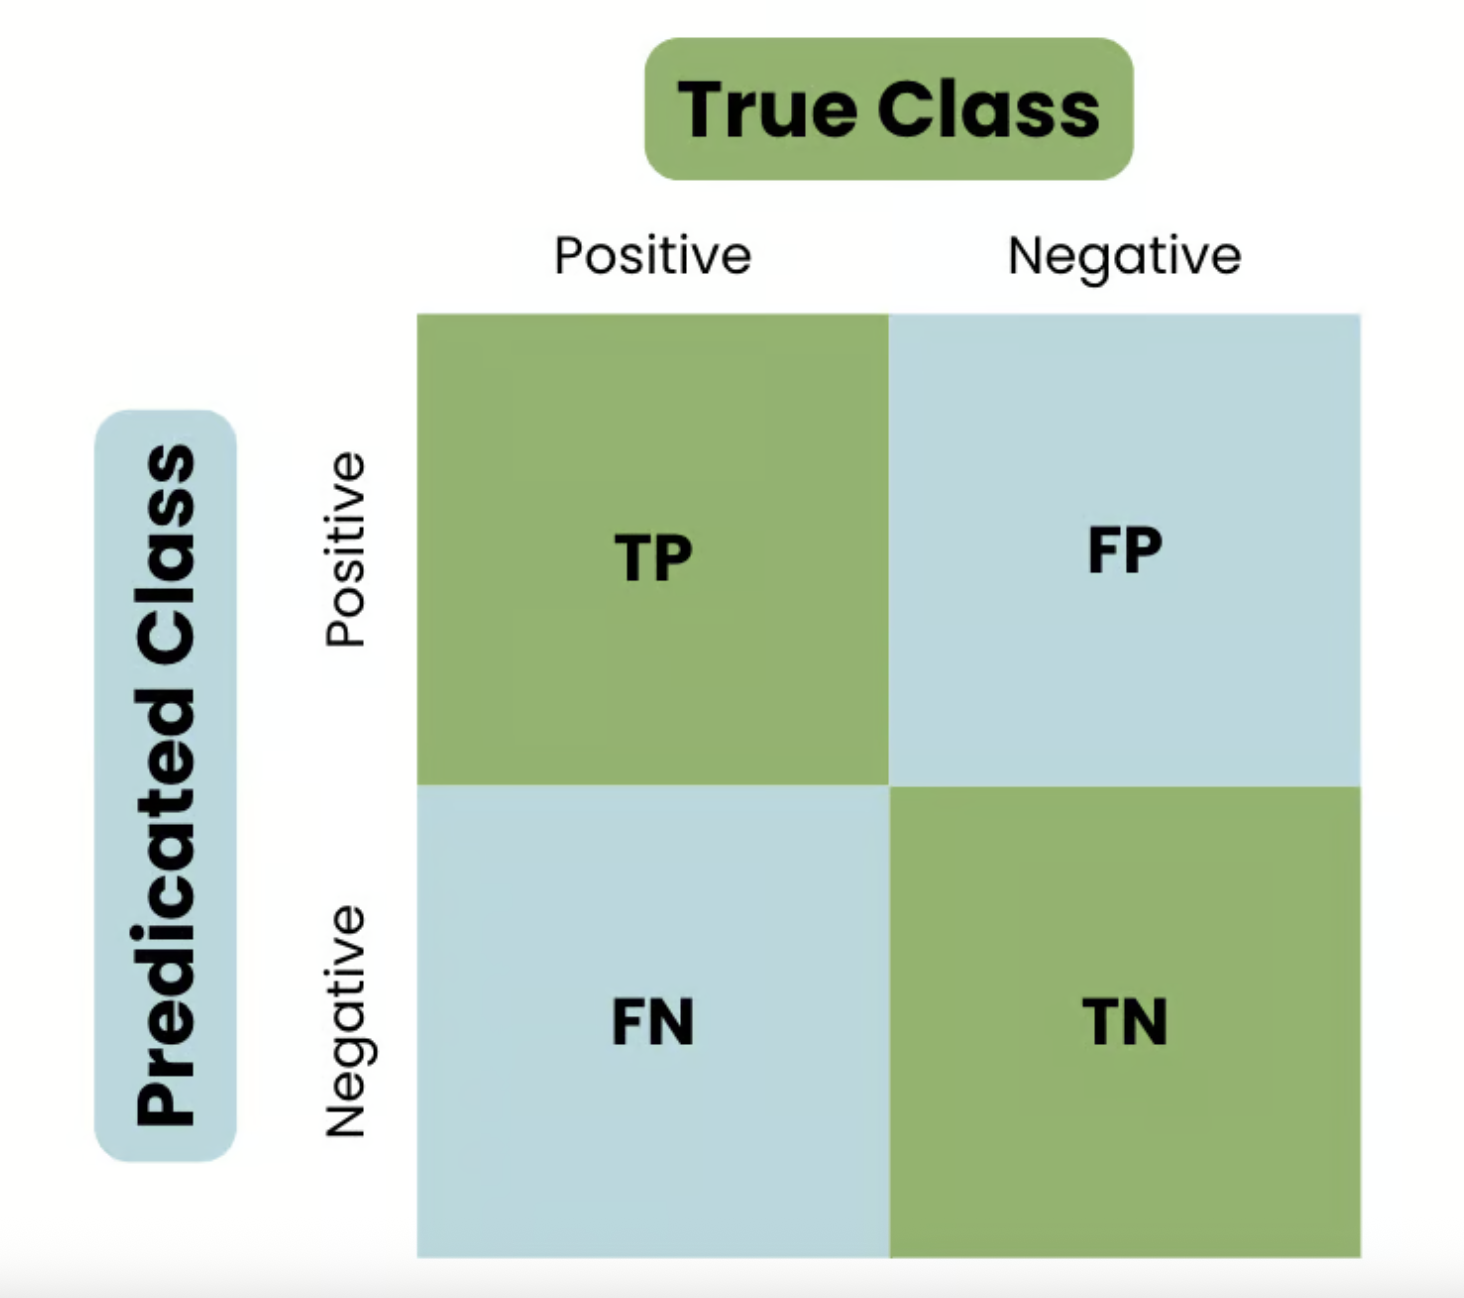
\includegraphics[scale=0.3]{static/confusion_matrix.png}
        \caption[Konfusionsmatrix]{\label{fig:confusion_matrix} Konfusionsmatrix\footnotemark}
    \end{center}
\end{figure}
\footnotetext{\url{https://www.datacamp.com/de/tutorial/what-is-a-confusion-matrix-in-machine-learning}}

Nach \cite{kivimaeki2025, Rainio:2024aa} sind die relevantesten Metriken für binäre Klassifikationen Accuracy, Recall (Sensitivity in \cite{Rainio:2024aa}), 
Specificity und Precision. 

\subsubsection{Accuracy}

Die Accuracy gibt den Anteil korrekt klassifizierter Instanzen an.

\begin{equation}
    \text{Accuracy} = \frac{TP + TN}{TP + TN + FP + FN}
\end{equation}

\subsubsection{Recall}

Der Recall gibt den Anteil korrekt erkannter positiver Fälle an.

\begin{equation}
    \text{Recall} = \frac{TP}{TP + FN}
\end{equation}

\subsubsection{Specificity}

Die Specificity gibt den Anteil korrekt erkannter negativer Fälle an.

\begin{equation}
    \text{Specificity} = \frac{TN}{TN + FP}
\end{equation}

\subsubsection{Precision}

Die Präzision gibt den Anteil tatsächlich positiver Fälle unter allen als positiv vorhergesagten Fällen an.

\begin{equation}
    \text{Precision} = \frac{TP}{TP + FP}
\end{equation}

\subsubsection{F1-Score}

Der F1-Score vereint die beiden Metriken Recall und Precision in einem einzigen Wert und ist hilfreich, wenn ein Gleichgewicht zwischen 
diesen beiden wichtig ist – vor allem bei unausgeglichenen Datensätzen, bei denen Accuracy allein irreführend sein kann.

Sind in dem Datensatz der Fake News Erkennung zum Beispiel 95\% der Artikel 'wahr' und 5\% 'falsch' hat ein Modell das ausschließlich
'wahr' vorhersagt eine Accuracy von 95\%. Es erkennt aber keinen einzigen Artikel der Fake ist.
Der Recall wäre in diesem Fall 0 und somit auch der F1-Score.

\begin{equation}
\text{F1\text{-}Score} = \frac{2 \cdot \text{Precision} \cdot \text{Recall}}{\text{Precision} + \text{Recall}}
\end{equation}


\section{Deep Learning}
\label{sec:deep_learning}

\subsection{Word Embeddings}
\label{sec:word_embeddings}

Die klassischen Merkmalsextraktionen in Kapitel \ref{sec:merkmalextraktion} eignen sich gut für klassische Machine Learning Modelle, wie
Support Vector Machines oder Logistische Regression.
Im Vergleich zu Word Embeddings erfassen diese aber keine semantischen Beziehungen.
Word Embeddings verstehen die Bedeutung der einzelnen Wörter je nach Word Embedding in Teilen oder im gesamten Kontext \cite{Deshai:2023aa}
und repräsentieren dabei das ursprüngliche Wort in einem neuen Vektorraum, wobei aber die Eigenschaften des Wortes und seine Verbindungen 
zu anderen Wörtern bestmöglich bewahrt werden \cite{Schaer2023}.
Dabei werden mit maschinellen Lerntechniken verschiedene dichte Vektoren mit einer festgelegten Dimension gebildet.
Word Embeddings sind gegenüber zu BOW (Sparse Matrizen) deutlich speicherschonender.

Das Wort „Bank“ zum Beispiel hat in den Sätzen „Ich setze mich auf die Bank.“ und „Ich raube die Bank aus.“ zwei unterschiedliche Bedeutungen. 
Moderne Word Embeddings erkennt diese und erstellt für die zwei Kontexte/Wörter zwei verschiedene Vektoren \cite{skopos2023wordembeddings}.

In Abbildung \ref{fig:bsp_word_embeddings} wird jedes Wort eines Korpus mit 6 Wörtern als dreidimensionaler Vektor dargestellt.
Ziel von Word2Vec ist hierbei, dass Wörter mit ähnlichen Bedeutungen oder Kontexten ähnliche Vektordarstellungen haben. 
Die Ähnlichkeit der Vektoren „Katze“ und „Hund“ zeigt die semantische Beziehung zueinander. Die Vektoren „glücklich“ und „traurig“ 
hingegen zeigen in entgegengesetzte Richtungen, was auf ihre gegensätzlichen Bedeutungen hinweist \cite{ibm2024wordembeddings}.

\begin{figure}[htbp]
    \begin{center}
        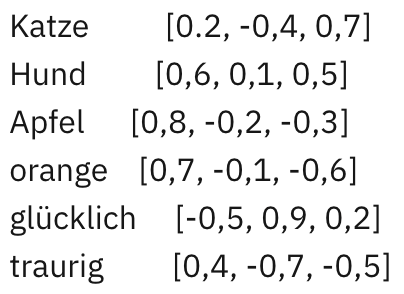
\includegraphics[scale=0.6]{static/bsp_word_embeddings.png}
        \caption{\label{fig:bsp_word_embeddings} Bsp. für Word Embeddings in einem dreidimensionalen Vektorraums \cite{ibm2024wordembeddings}}
    \end{center}
\end{figure}

\subsubsection{Word2Vec}
\label{sec:word2vec}

Das Word Embedding Word2vec verwendet ein neuronales Netzwerk und erfasst numerisch die Ähnlichkeiten zwischen Wörtern aufgrund ihrer 
kontextuellen Merkmale. Am häufigsten wird sie zur Analyse der semantischen Verbindungen zwischen Wörtern in einem Textkorpus 
eingesetzt \cite{schumacher2024word2vec}.

Im Beispielsatz 'Mann verhält sich zu Frau wie König zu x.' erkennt Word2vec, dass für $x = \text{Königin}$ gilt. 
Word2Vec löst solche Aufgaben, indem es alle Wörter $x'$ im Gesamtvokabular $V$ ausprobiert 
und das Wort findet, das folgende Gleichung maximiert \cite{CHURCH_2017}:

\begin{equation}
    \hat{x} = \underset{x' \in V}{\operatorname{argmax}} \; \text{sim}(x', \vec{\text{king}} + \vec{\text{woman}} - \vec{\text{man}})
\end{equation}

Wie in Abbildung \ref{fig:cbow_skipgram} zu sehen, gibt es für Word2Vec zwei verschiedene Implementierungen.
Im CBOW-Modell (continuous bag-of-words) wird ein Wort aufgrund seines Kontextes vorhergesagt.
Im Skip-gram-Modell wird hingegen Kontexte aufgrund eines Wortes vorhergesagt.

Bei einem relativ kleines Korpus, empfiehlt Google aufgrund seiner ausgeprägten Fähigkeit mit niedrigfrequenten Wörtern zu arbeiten, 
das Skip-gram-Modell anzuwenden \cite{schumacher2024word2vec}.

\begin{figure}[htbp]
    \begin{center}
        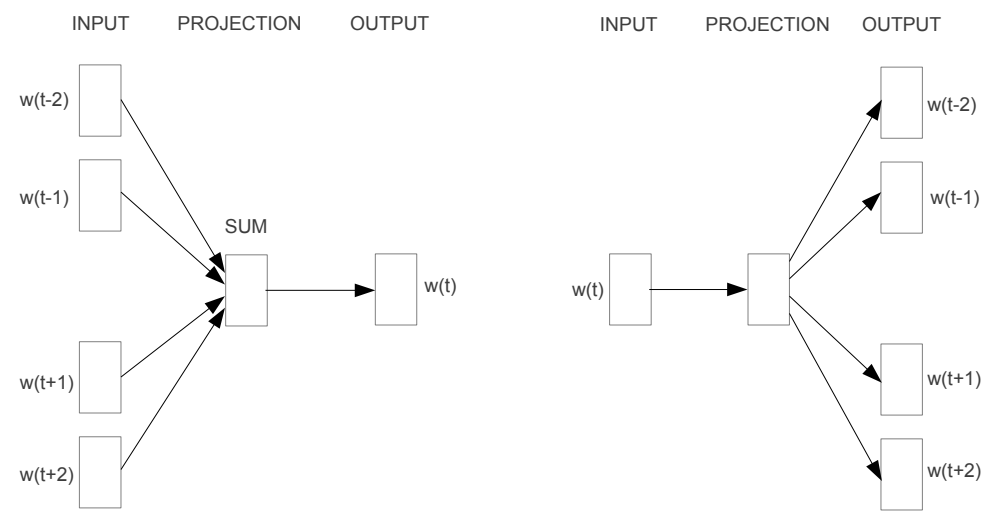
\includegraphics[scale=0.6]{static/cbow_skipgram.png}
        \caption{\label{fig:cbow_skipgram} Vergleich CBOW (links) und Skip-gram (rechts) \cite{mikolov2013}}
    \end{center}
\end{figure}

\subsubsection{GloVe}

Word2Vec fokussiert sich auf Informationen aus lokalen Kontextfenster, wobei globale Informationen hierbei nicht ausreichend genutzt werden.
GloVe (Global Vectors for Word Representation) verwendet diese globalen Informationen, wodurch semantische Beziehungen zwischen Wörtern erfasst werden.
Wie oft diese zusammen im Korpus vorkommen, wird in einer globalen Co-Occurrence-Matrix zusammengefasst \cite{Wang:2020aa}.

Sei $X$ eine Co-Occurrence-Matrix.
Für jedes Wortpaar $(i, j)$ zeigt $X_{ij}$, wie häufig das Wort $w_j$ im Kontext von $w_i$ erscheint.

Die bedingte Wahrscheinlichkeit, dass Wort $j$ im Kontext von $i$ erscheint, ist:

\begin{equation}
    P(j \mid i) = \frac{X_{ij}}{X_i}
\end{equation}

\begin{figure}[htbp]
    \begin{center}
        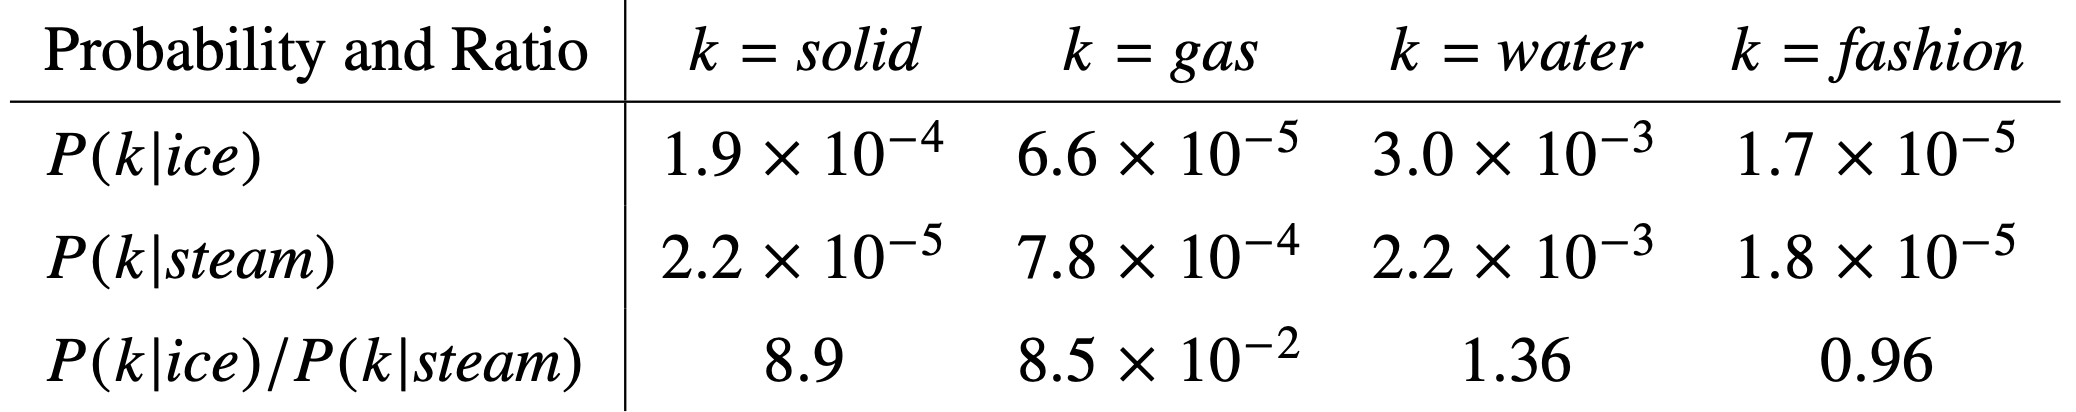
\includegraphics[scale=0.3]{static/glove_matrix.png}
        \caption{\label{fig:glove_matrix} Co-Occurrence-Wahrscheinlichkeiten für die Zielwörter „ice“ und „steam“ mit ausgewählten Kontextwörtern aus einem Korpus mit 6 Milliarden Tokens \cite{pennington2014glove}}
    \end{center}
\end{figure}

Zur Modellierung semantischer Beziehungen vergleicht GloVe Wahrscheinlichkeitsverhältnisse:

\[
\frac{P_{ik}}{P_{jk}} = \frac{X_{ik} / X_i}{X_{jk} / X_j}
\]

In Abbildung \ref{fig:glove_matrix} zu erkennen ist, dass Werte > 1 gut mit Eigenschaften, die spezifisch für „ice“ sind
und Werte < 1 gut mit Eigenschaften, die spezifisch für „steam“ sind korrelieren.
Für $k=solid$ ist der Quotient 8.9. „solid“ hat somit eine größere semantische Beziehung mit „ice“ als mit „steam“.
Für $k=gas$ ist der Wert 0.085. „gas“ passt folglich besser zu „steam“ als zu „ice“.


\subsection{Deep Learning-Modelle}
\label{sec:deep_learning_modelle}

\subsubsection{CNN vs. RNN}

Ein Convolutional Neural Network (CNN) ist ein Deep Learning Model (DNN) für Klassifikationsaufgaben,
das Eingabedaten analysiert und dabei unterschiedlichen Merkmalen innerhalb der Daten Gewichtungen zuweist,
um charakteristische Muster zu erkennen und verschiedene Klassen voneinander zu unterscheiden.
Ein großer Vorteil von CNNs ist, dass sie wenig Datenvorverarbeitung benötigen, da sie Rohdaten direkt als Eingabe verarbeiten 
können \cite{aslam2022}.

Ein Recurrent Neural Network (RNN) ist ein DNN zur Verarbeitung sequentieller Daten.
Im Vergleich zu CNNs können sich RNNs an frühere Eingaben erinnern, um aktuelle Vorhersagen zu beeinflussen \cite{Deshai:2023aa}.
RNN nutzt dabei den aktuellen Eingabewert sowie den vorherigen Ausgabewert in jedem Zeitschritt 
und trainiert sich damit selbst, indem es Fehler der Ausgabe zur Eingabe hinzu berechnet.
RNN eignet sich somit besonders für Probleme in der natürlichen Sprachverarbeitung \cite{Wang:2020aa}, 
da die Reihenfolge der Elemente in diesem Fall entscheidend ist.

Ein zentrales Problem bei RNNs ist jedoch das sogenannte Vanishing Gradient Problem, welches das Lernen 
langer Datenfolgen stark einschränken kann \cite{aslam2022}.

\subsubsection{LSTM}

Long Short-Term Memory (LSTM), ein RNN-Typ im Bereich der Sprachverarbeitung. Das Modell behebt das Problem des 
Vanishing Gradient Problems in klassischen RNNs, indem sie spezielle Speicherzellen verwenden, die Informationen über 
längere Zeiträume hinweg behalten können.
Dadurch sind die LSTM-Modelle effektiv darin, langfristige Abhängigkeiten in sequenziellen Daten zu erfassen und
Beziehungen zwischen Wörtern zu identifizieren \cite{Deshai:2023aa}.

Ein LSTM-Modell besteht aus mehreren Zellen, die nicht nur eine, sondern drei Aktivierungsfunktionen enthalten.
Jede dieser Zellen speichert den Zustand des Problems über mehrere Zeitintervalle, während die drei Tore den 
Informationsfluss in die Zelle hinein und aus ihr heraus regulieren.
Das Input-Gate, das Output-Gate und das Forget-Gate \cite{berrajaa2022nlp} (siehe Abbildung \ref{fig:rnnvslstm}).

\begin{figure}[htbp]
    \begin{center}
    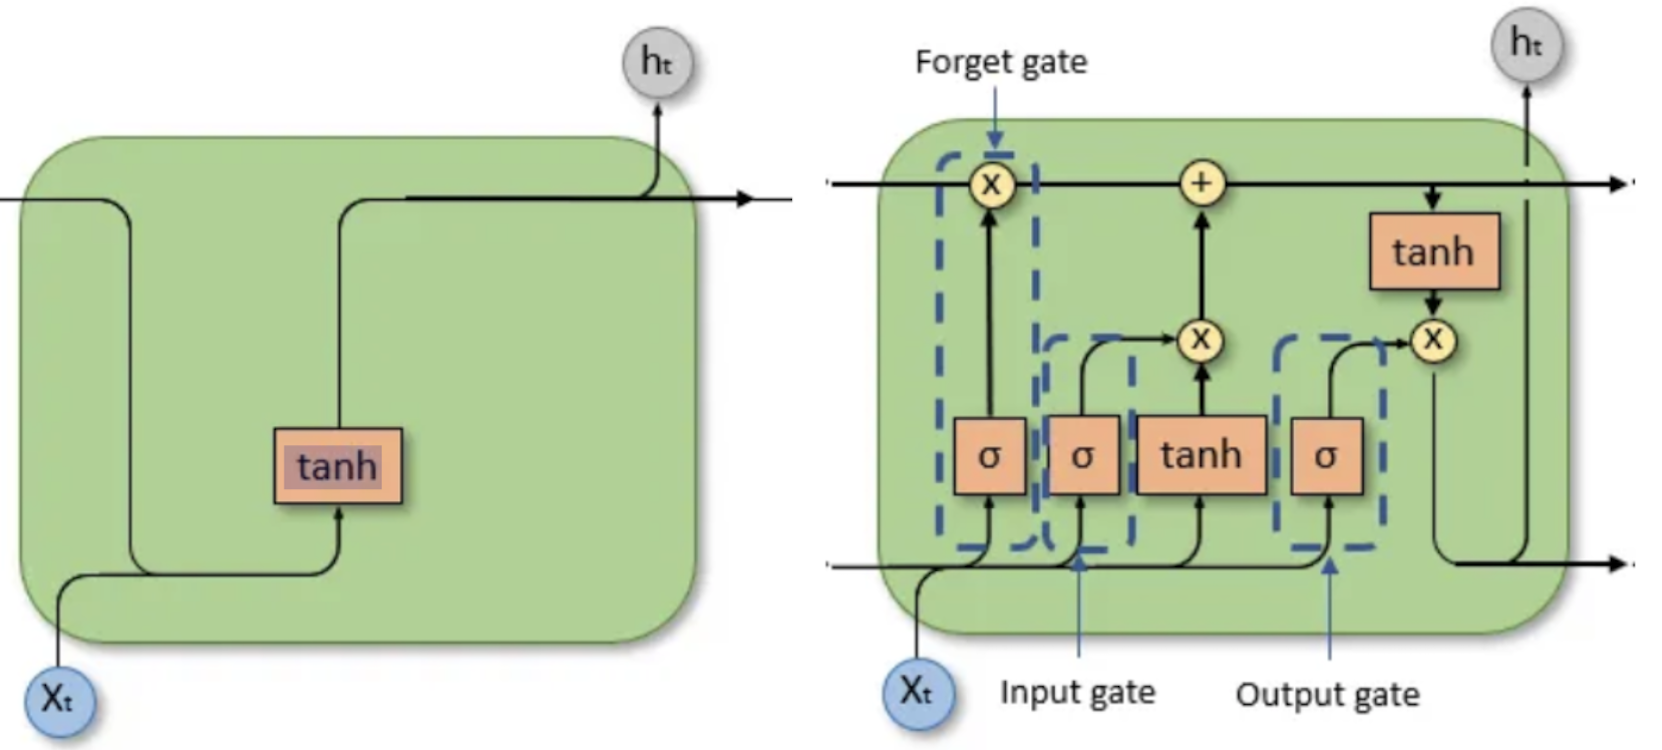
\includegraphics[scale=0.4]{static/RNNvsLSTM.png}
    \caption{\label{fig:rnnvslstm} Vgl. RNN (links) und LSTM (rechts) \cite{aiml2025sequence}}
    \end{center}
\end{figure}

Das Forget-Gate bestimmt, welche Informationen nicht mehr relevant sind und gelöscht werden können. 
Dies hilft, den Speicher der Zelle zu optimieren und unnötige Daten zu entfernen.

Das Input- und Output-Gate bestimmen, welche neuen Daten hinzugefügt und welche bestehenden 
Daten ausgegeben werden sollen. Sie arbeiten zusammen, um den Informationsfluss zu regulieren.

\subsubsection{BiLSTM}

\begin{figure}[htbp]
    \begin{center}
        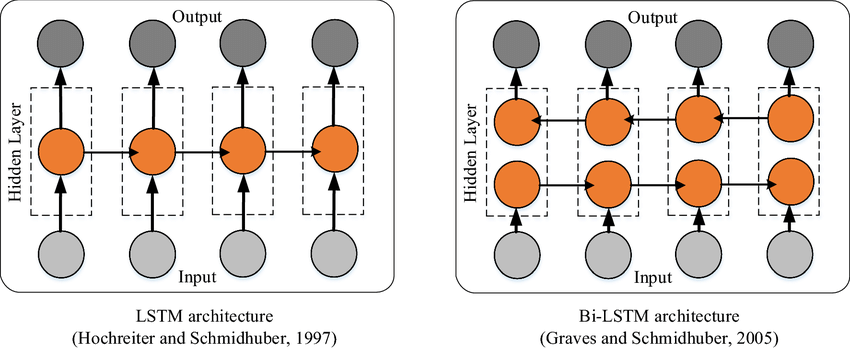
\includegraphics[scale=0.4]{static/lstmvsbilstm.png}
        \caption{\label{fig:lstmvsbilstm} Vgl. LSTM und BiLSTM \cite{shen2021}}
    \end{center}
\end{figure}

Bidirectional-LSTMs (BiLSTMs) sind eine Erweiterung der LSTM-Modelle, bei der zwei LSTMs auf die Eingabedaten angewendet werden. 
In der ersten Runde wird der Input von der ersten LSTM verarbeitet. Anschließend wird der Input in umgekehrter Form auf die zweite LSTM
angewendet (siehe Abbildung \ref{fig:lstmvsbilstm}). Der Input wird somit vor- und rückwärts gelesen, was das Erlernen von 
Langzeitabhängigkeiten verbessert und zu einer höheren Genauigkeit des Modells führt \cite{siaminamini2019}. 

Der Hauptunterschied zwischen Bi-LSTMs und LSTMs besteht daher darin, dass Letztere nur 
Informationen aus der Vergangenheit bewahren, während in Bi-LSTMs durch die Kombination der beiden verborgenen Zustände sowohl Informationen 
aus der Vergangenheit als auch aus der Zukunft zu jedem Zeitpunkt erhalten bleiben können \cite{shen2021}.


\subsubsection{BERT} \label{sec04:bert}

Bidirectional Encoder Representations from Transformers (BERT) ist eine Form der Transformer.
Diese sind erweiterte Deep-Learning-Modelle, welche sich aus einem Encoder und einem Decoder zusammensetzen (siehe Abbildung 
\ref{fig:transformeroverview}) und den sogenannten Self-Attention Mechanismus nutzen \cite{vaswani2023attentionneed}.

\begin{figure}[htbp]
    \begin{center}
    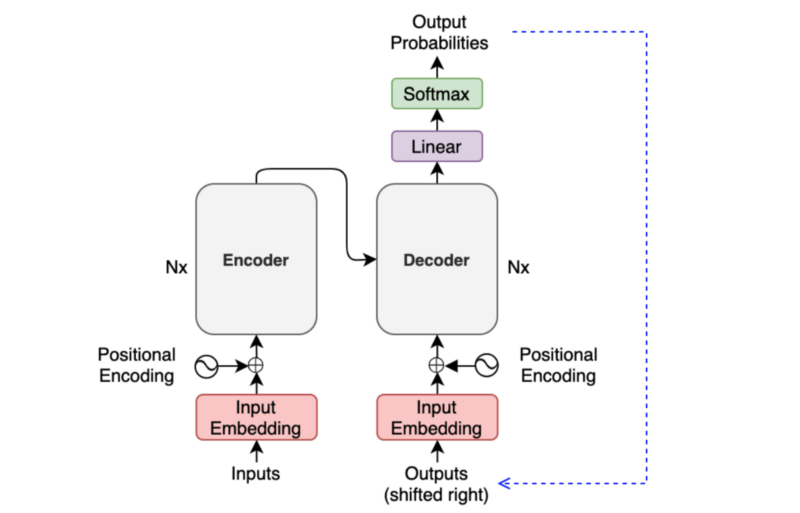
\includegraphics[scale=0.4]{static/transformer-overview.png}
    \caption{\label{fig:transformeroverview} Eine Übersicht der Transformer Architektur \cite{kikaben2021transformer} 
    - vereinfacht von \cite{vaswani2023attentionneed}}
    \end{center}
\end{figure}

Dieser Mechanismus, betrachtet für jedes Wort in einer Sequenz alle anderen Wörter, um zu entscheiden, 
wie wichtig sie für seine Bedeutung sind.
In dem Satz „Die Bank hat heute geschlossen.“ erkennt Self-Attention zum Beispiel, dass „Bank“ im Kontext von „geschlossen“ eher ein Gebäude 
und kein Möbelstück ist. %TODO: bsp erzeugt durch scholargpt
Im Vergleich zu RNNs, welche Kontexte nur von links nach rechts erkennen können (bzw. bi-direktional in BiLSTMs) kann der Kontext in Transformern
global erkannt werden \cite{ghojogh2020}.

Angenommen der Transformer würde zum maschinellen Übersetzen eines Textes genutzt werden, dann besitzt das Encoding das Sprachverständnis, 
während das Decoding die Texgenerierung vornimmt. BERT ist ein reiner, für Sprachverständnis optimierter, Encoder-Transformer \cite{devlin2019}.

Während CNNs und RNNs externe Word Embeddings wie Word2Vec oder GloVe verwenden, nutzt BERT eigene lernbare Embeddings.
Dazu noch einmal das Beispiel aus Kapitel \ref{sec:word_embeddings}: „Ich setze mich auf die Bank.“ und „Ich raube die Bank aus.“

GloVe und Word2Vec erstellen einen festen Vektor für das Wort „Bank“, egal in welchem Satz es steht.
Bei GloVe ist dieser Vektor ein Mittelwert aus allen Bedeutungen, die „Bank“ im Korpus je hatte.
Der Vektor liegt folglich irgendwo zwischen Sitzmöbel und Finanzinstitut und repräsentiert keine der beiden Bedeutungen exakt.

BERT löst dieses Problem indem es kontextabhängige Embeddings erzeugt. So wird ein Vektor für das Wort „Bank“ erzeugt, der zur Bedeutung
Sitzmöbel passt und ein weiterer für die Bedeutung Finanzinstitut.

Es verwendet während des Trainings Masked Language Modeling (MLM), um den Kontext und die Bedeutung von Wörtern im Satz zu verstehen.
Anschließend wird es auf einem Datensatz mit gelabelten Bewertungen feinjustiert. 
Dabei verbindet es jedes Eingabeelement mit jedem Ausgabeelement und 
weist dabei wichtigen Wörtern und Phrasen im Text höhere Gewichtungen zu \cite{Deshai:2023aa}.

Im MLM wird ein bestimmer Teil der Wörter in der Eingabesequenz zufällig maskiert (siehe Abbildung \ref{fig:mlm_bert}), 
und das Modell muss diese verdeckten Wörter korrekt vorhersagen.

\begin{figure}[htbp]
    \begin{center}
        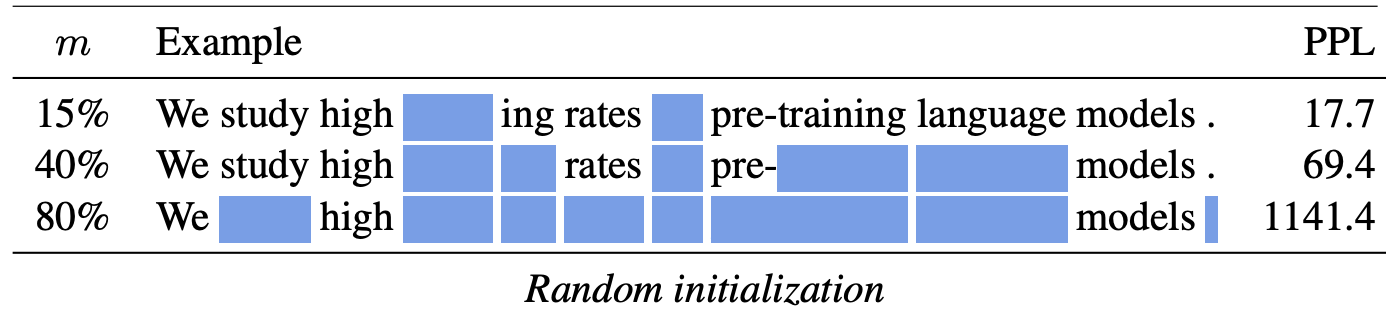
\includegraphics[scale=0.5]{static/mlm_bert.png}
        \caption{\label{fig:mlm_bert} Bsp. zum MLM \cite{wettig2023}}
    \end{center}
\end{figure}

Aufgrund der Bidirektionalität des BERT Modells ist dieses bei späteren Vorhersagen effektiver \cite{wettig2023}. 
\cite{devlin2019} zeigt, wie relevant bidirektionalen Pretrainings für qualitativ hochwertige Sprachrepräsentationen sind.

BERT nutzt die bi-direktionale Transformer-Architektur (siehe Abbildung \ref{fig:architecture_bert}), bei welcher tiefe semantische Informationen 
eines Satzes erfasst werden können.
Der Vorteil besteht darin, dass die gelernten Repräsentationen den Kontext in beide Richtungen integrieren können \cite{Wang:2020aa}.

\begin{figure}[htbp]
    \begin{center}
        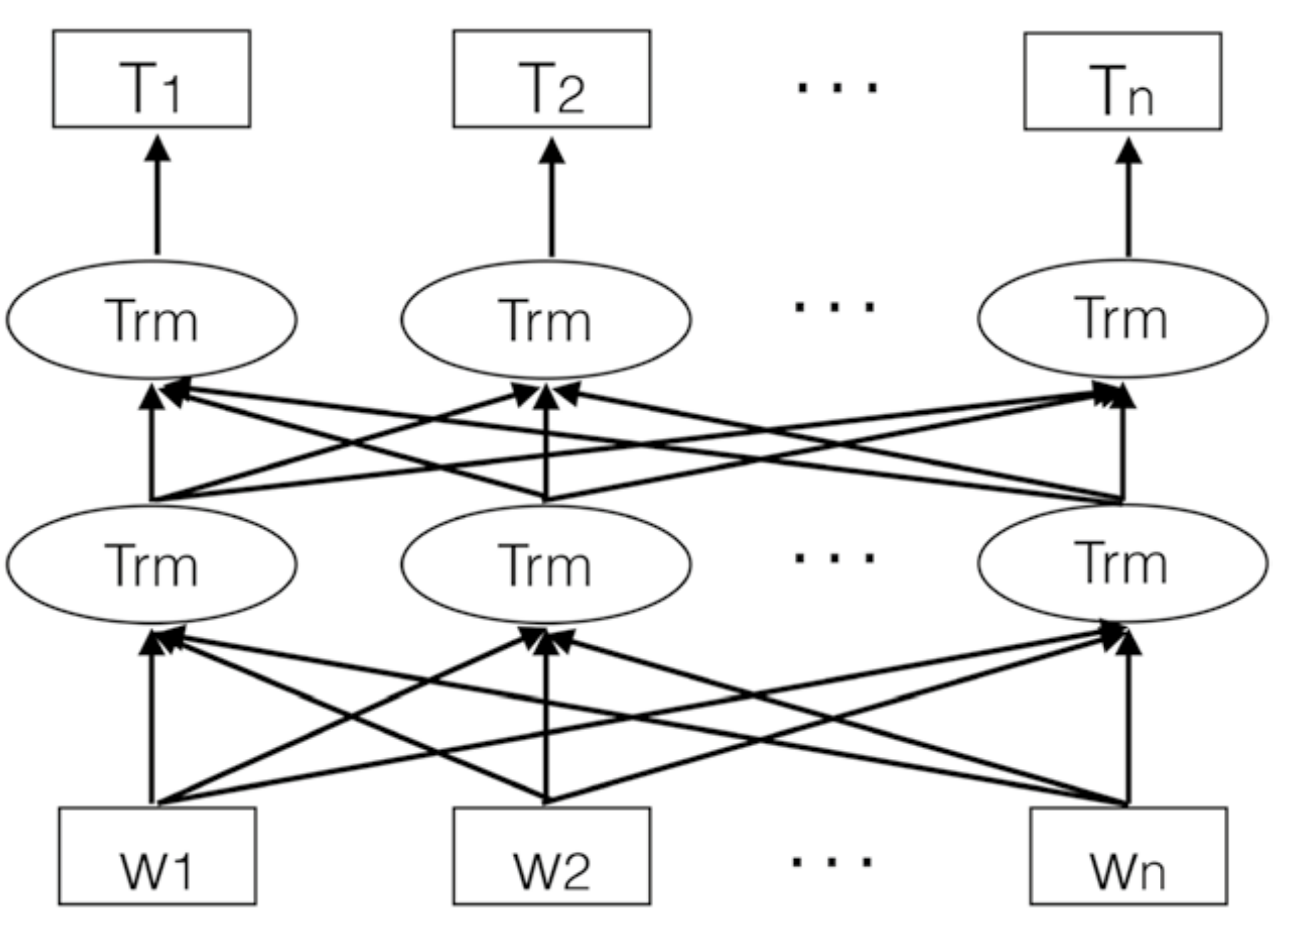
\includegraphics[scale=0.3]{static/architecture_bert.png}
        \caption{\label{fig:architecture_bert} Architektur des BERT Modells \cite{Wang:2020aa}}
    \end{center}
\end{figure}

Für das Erstellen der Wortvektoren werden bei diesem Embedding WordPiece Embeddings genutzt.
Es wurde von Google speziell für BERT entwickelt, um auch seltene oder unbekannte Wörter sinnvoll verarbeiten zu können.
WordPiece ist ein Tokenisierungsverfahren, das Wörter in kleinere Einheiten zerlegt.

Folgendes Beispiel für ein WordPiece Embedding (aus \cite{huggingface2025wordpiece}):
\begin{enumerate}
    \item Das \textbf{Startvokabular} besteht aus einem Vokabular aus Einzelbuchstaben 
    (z.B. \texttt{h}, \texttt{\#\#e}, \texttt{\#\#l}, \texttt{\#\#o} für ``hello''), 
    wobei alle Buchstaben außer dem Ersten mit \texttt{\#\#} markiert werden, um zu zeigen, dass sie nicht am Wortanfang stehen.

    \item \textbf{Häufigkeitsanalyse:} Identifiziert häufig gemeinsam auftretende Buchstabenpaare, 
    z.B. \texttt{("\#\#g", "\#\#s")} in ``hugs''.

    \item \textbf{Mergeregeln:} Zum Zusammenfügen berechnet WordPiece einen Score:

    \begin{equation}
        \text{Score} = \frac{\text{Häufigkeit des Paares}}{\text{Häufigkeit Teil 1} \times \text{Häufigkeit Teil 2}}
    \end{equation}

    Dadurch werden eher seltene Kombinationen zusammengefügt, die besser charakteristische Subwörter ergeben.

    \item \textbf{Merge-Iterationen:} Das Zusammenfügen wird so lange wiederholt, bis das gewünschte Vokabular erreicht ist.
\end{enumerate}

\textbf{Beim Zerlegen neuer Wörter:}
\begin{enumerate}
    \item Suche das längste Subwort im Vokabular, das am Wortanfang passt.
    \item Markiere alles danach mit \texttt{\#\#} und wiederhole.
    \item Wenn gar kein Teil im Vokabular ist, kommt das Sondertoken \texttt{[UNK]} (unbekannt) zum Einsatz.
\end{enumerate}

\textbf{Beispiele:}
\begin{itemize}
    \item \texttt{"hugs"} $\rightarrow$ \texttt{["hug", "\#\#s"]}
    \item \texttt{"bugs"} $\rightarrow$ \texttt{["b", "\#\#u", "\#\#gs"]}
    \item \texttt{"mug"} $\rightarrow$ \texttt{[UNK]}, falls \texttt{\#\#m} nicht im Vokabular ist
\end{itemize}

Zusätzlich werden Positions- und Segment-Embeddings hinzugefügt (siehe Abbildung \ref{fig:bert_tokenizierung}).

\begin{figure}[htbp]
    \begin{center}
        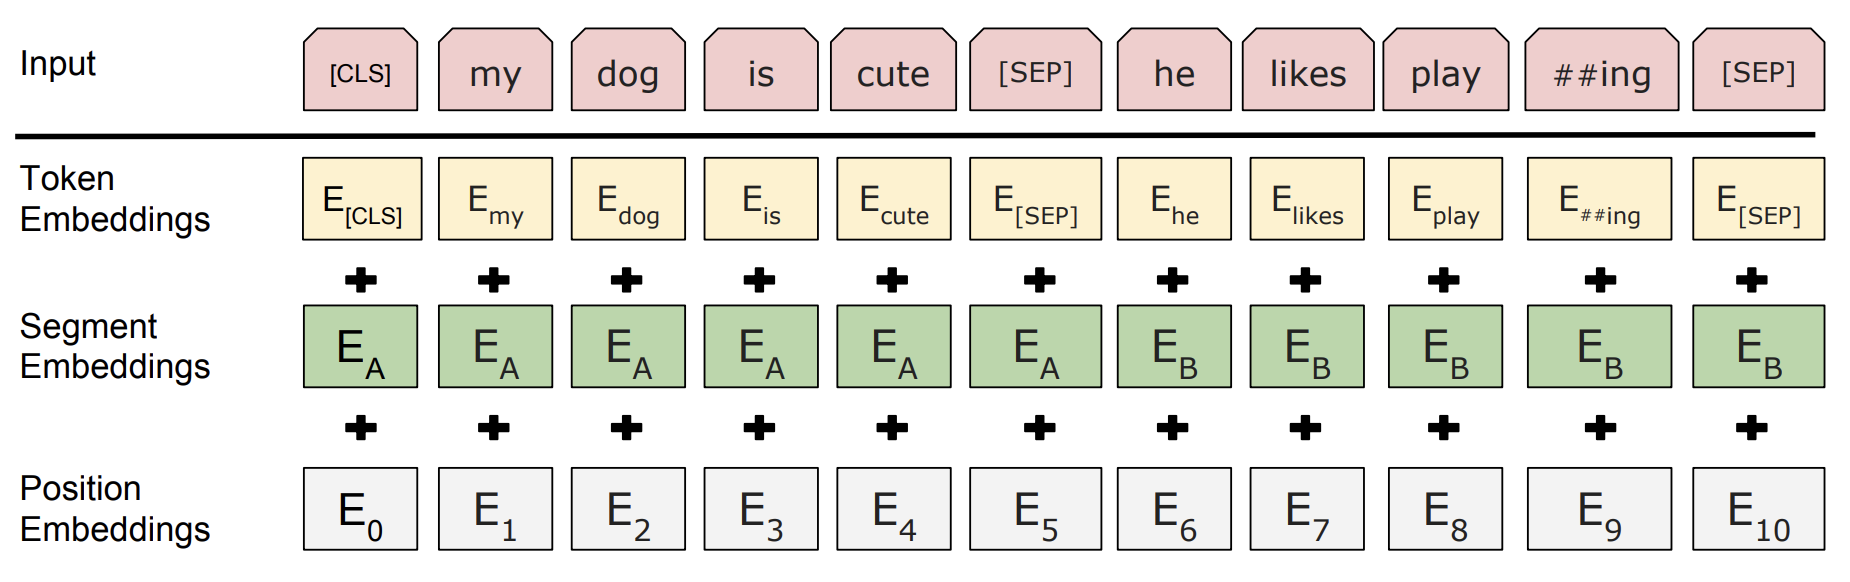
\includegraphics[scale=0.4]{static/bert_tokenizierung.png}
        \caption{\label{fig:bert_tokenizierung} Zusammensetzung eines Input Tokens im BERT Modell \cite{devlin2019}}
    \end{center}
\end{figure}

Das Input Token ergibt sich aus dem Token-, Position- und Segment-Embedding. Das Position-Embedding (Position Encoding in Abbildung \ref{fig:transformeroverview}) 
stellt hierbei die jeweilige Position im Satz dar und das Segment-Embedding ordnet den Token dem entsprechenden Satz zu.

\section{Hybride Modelle für Fake News Erkennung}
\label{sec:hybride_modelle}

\subsection{CNN und LSTM mit PCA}

In \cite{umer2020} wird eine hybride neuronale Netzwerkarchitektur vorgeschlagen, die die Fähigkeiten von CNN und 
LSTM kombiniert. Dabei kommen zwei unterschiedliche Verfahren zur Dimensionsreduktion zum Einsatz: 
Hauptkomponentenanalyse (PCA) und Chi-Quadrat-Verfahren. 
Diese Verfahren werden empfohlen, um die Dimensionalität der 
Merkmalsvektoren zu verringern, bevor diese an den Klassifikator weitergeleitet werden.

\begin{figure}[htbp]
    \begin{center}
    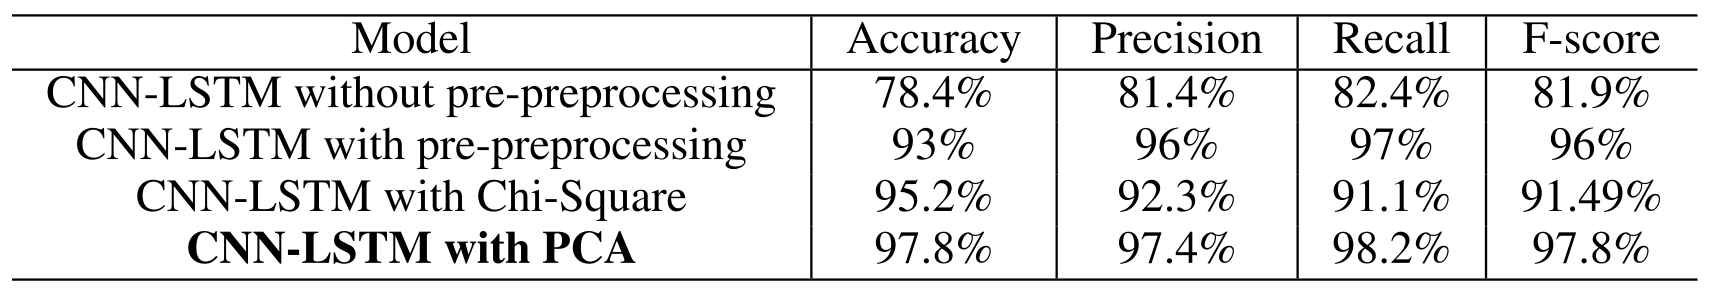
\includegraphics[scale=0.4]{static/cnn_lstm_pca.png}
    \caption{\label{fig:cnn_lstm_pca} Ergebnisse der Klassifizierungen der verschiedenen CNN-LSTM Modelle \cite{umer2020}}
    \end{center}
\end{figure}

Wie in Abbildung \ref{fig:cnn_lstm_pca} zu erkennen, werden verschiedenen Modelle miteinander verglichen. Einmal mit und ohne Vorverarbeitung
der Daten und dann mit den verschiedenen Dimensionsreduktionen PCA und Chi-Quadrat.
PCA schneidet mit einem F1-Score von 97,8\% am Besten ab, während keine Vorverarbeitung der Daten nur einen F1-Score von 81,9\% erreicht.

Die Modelle wurden auf Basis des FNC-1 Datensatzes gemessen, in welchem 2.587 Artikeln etwa 300 verschiedenen Schlagzeilen zugeordnet werden sollen.
Jeder Artikel wird in Bezug auf eine Schlagzeile einer von vier Klassen zugeordnet:

\begin{itemize}
    \item \textbf{Agree:} Artikel stimmt der Schlagzeile zu
    \item \textbf{Disagree:} Artikel widerspricht der Schlagzeile
    \item \textbf{Discuss:} Artikel diskutiert das Thema der Schlagzeile
    \item \textbf{Unrelated:} Artikel ist thematisch nicht verwandt mit der Schlagzeile
\end{itemize}

Zum Vergleich wurden weitere Modelle wie BERT auf den Datensatz angewendet.
Dieses erzielte eine Accuracy von 91,3\% während das hybride CNN-LSTM Modell eine Accuracy von 97,8\% erreichte.

\subsection{CNN und LSTM mit GloVe}

Ein weiteres in \cite{Buddhadev2025} vorgestelltes hybrides Modell ist zusammengesetzt aus CNN und LSTM. Zusätzlich werden die Daten
mit dem GloVe Embedding vorverarbeitet.

\begin{figure}[htbp]
    \begin{center}
    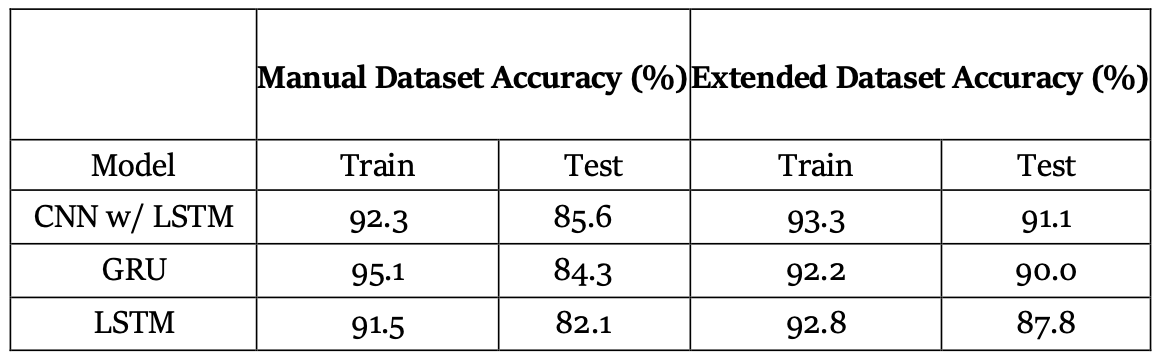
\includegraphics[scale=0.5]{static/cnn_lstm_glove.png}
    \caption{\label{fig:cnn_lstm_glove} Ergebnisse verschiedener Modelle mit GloVe Embedding \cite{Buddhadev2025}}
    \end{center}
\end{figure}

Getestet wurden die Modelle CNN mit LSTM, GRU und LSTM. Genutzt wurden zwei verschiedene Datensätze. Ein manuell erzeugter aus über 1500 Quellen basierend auf
ca. 9000 Artikeln mit Falschinhalten und ca. 9000 echten Artikeln und ein erweiteter, welcher zusätzlich mit Inhalten aus anderen Datensätzen von Kaggle oder
GitHub bereichert wurde.
Durch die zusätzliche Nutzung von GloVe Embeddings wird in dieser Arbeit das Overfitting reduziert (siehe Abbildung \ref{fig:cnn_lstm_glove}).
Vergleichsweise ist die Accuracy beim erweiterten Datensätz mit dem Keras Embedding bei 98,4\% im Training und bei 89,5\% beim Test (CNN mit LSTM).

\cite{Buddhadev2025} stellt außerdem fest, dass Wort-Embeddings wie GloVe die Semantik des Textes deutlich besser erfassen als Techniken zur Merkmalsextraktion 
wie Bag-of-Words oder TF-IDF. In Kombination mit Deep-Learning-Modellen liefern sie eine höhere Genauigkeit als herkömmliche Machine-Learning-Modelle.

\subsection{BERT und CNN (FakeBERT)}
\label{sec:fakebert}

Ein von \cite{Kaliyar:2021aa} vorgestelltes Modell trägt den Namen \textit{FakeBERT} und setzt sich aus den Modellen BERT und CNN zusammen.
BERT analysiert den Text und versteht den 
Zusammenhang der Wörter, während mehrere kleine CNNs gleichzeitig verschiedene Merkmale aus dem Text herausfiltern. Die Ergebnisse dieser 
CNNs werden zusammengeführt, weiterverarbeitet und klassifiziert. Entschieden wird auch in diesem Modell ob es sich um echte oder falsche 
Nachrichten handelt. Das Modell erkennt durch diese Architektur sowohl den allgemeinen Sinn als auch feine sprachliche Muster im Text.

Gearbeitet wurde mit dem \textit{fake-and-real-news-dataset} von Kaggle. Dieser besteht aus 20.800 Nachrichtenartikeln, die während der US-Präsidentschaftswahl 2016 gesammelt wurden. 
Enthalten sind unter anderem Merkmale wie Titel, Autor, Textinhalt. Klassifiziert werden die Nachrichten als echt oder gefälscht. 
Im Datensatz gibt es 10.540 echte und 10.260 gefälschte Artikel.

\begin{figure}[htbp]
    \begin{center}
    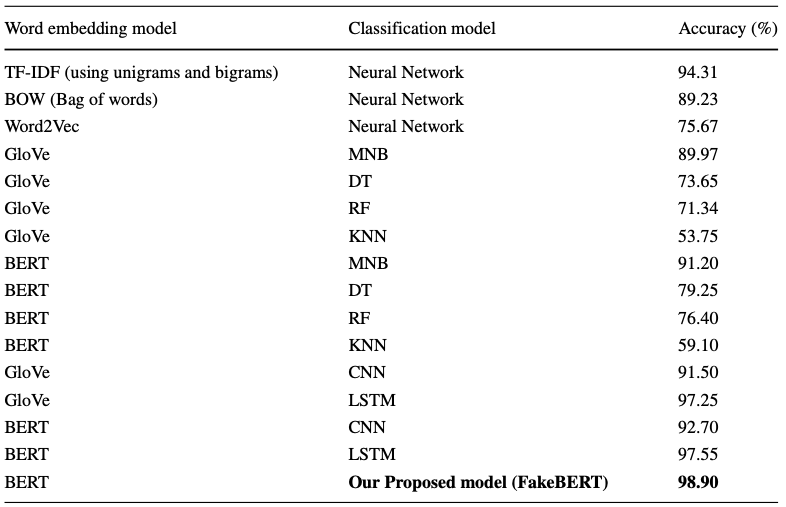
\includegraphics[scale=0.5]{static/bert_cnn_fakebert.png}
    \caption{\label{fig:bert_cnn_fakebert} Ergebnisse der verschiedenen Modelle bei Validierung \cite{Kaliyar:2021aa}}
    \end{center}
\end{figure}

\cite{Kaliyar:2021aa} zeigt, dass das vorgeschlagene Modell FakeBERT mit einer Genauigkeit von 98,90\% (siehe Abbildung \ref{fig:bert_cnn_fakebert} 
deutlich besser abschneidet als klassische Machine-Learning-Modelle und bis 2021 bestehende Deep-Learning-Ansätze. Durch die Kombination von BERT als 
kontextuelles Sprachmodell mit mehreren parallel laufenden CNN-Blöcken zur Merkmalsextraktion können sowohl globale Bedeutungszusammenhänge als auch 
lokale sprachliche Muster zuverlässig erfasst werden.

\subsection{BERT und CNN (MCred)}

Wie auch in Kapitel \ref{sec:fakebert} entwickelt \cite{Verma:2023aa} in seiner Arbeit ein weiteres hybrides Modell aus BERT und CNN.
Dieses trägt den Namen \textit{MCred}.

Es wird auf vier verschiedenen Datensätzen trainiert:
\begin{itemize}
  \item \textbf{WELFake:} Enthält 37.106 gefälschte und 35.028 echte Nachrichten und dient als Hauptdatensatz für das MCred-Modell.
  \item \textbf{Kaggle Fake News Dataset:} Umfasst 10.369 gefälschten und 10.349 echte Nachrichten mit den Merkmalen Titel, Text und Autor. 
  \item \textbf{McIntire Dataset:} Besteht aus 3.164 gefälschten und 3.171 echten Nachrichtenartikeln zur US-Präsidentschaftswahl 2016.
  \item \textbf{FakeNewsNet:} Enthält 24.396 gefälschte und 13.614 echte Nachrichten. Stammt aus diversen Quellen und deckt zahlreiche Themenfelder ab.
\end{itemize}

FakeBERT kombiniert BERT direkt mit parallelen CNNs zur Merkmalsextraktion, während MCred BERT und CNN getrennt verarbeitet und 
ihre Ausgaben später zusammenführt. Zudem nutzt MCred zusätzlich GloVe-Embeddings, was FakeBERT nicht tut. 
Wie in Abbildung \ref{fig:bert_cnn_mcred} zu erkennen erreicht MCred dadurch im Kaggle Datensatz mit einer Accuracy von 99,46\% 
einen besseren Wert als FakeBERT (Rohit Kumar Kaliyar and Narang (2021)) mit 98,90\%.

\begin{figure}[htbp]
    \begin{center}
    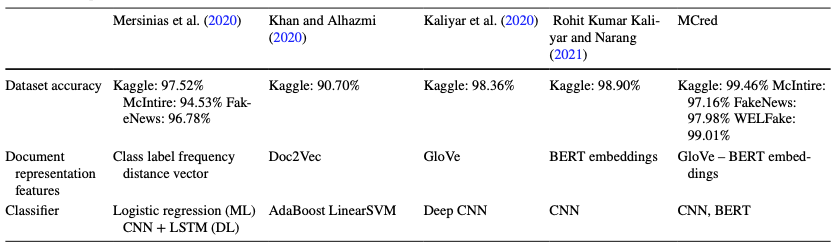
\includegraphics[scale=0.49]{static/bert_cnn_mcred.png}
    \caption{\label{fig:bert_cnn_mcred} Ergebnisse der verschiedenen Modelle \cite{Verma:2023aa}}
    \end{center}
\end{figure}

In \cite{Dhiman:2024aa} wurde MCred im August 2024 mit einer Accuracy von 99,01\% als zweitbeste State-of-the-Art-Technik benannt.

\subsection{BERT und LSTM}

\cite{RAI202298} schlägt ein hybrides Modell vor, welches BERT und LSTM kombiniert. Hierbei fungiert BERT nachdem die Daten bereinigt wurden als Tokenizer und
Basismodell durch seine Fähigkeit zur tiefen und kontextuellen Wortrepräsentationen (siehe Abbildung \ref{fig:bert_lstm_architecture}). 
Anschließend werden die erzeugten Embeddings in ein LSTM gegeben, in welchem dessen Zellen die Langzeitabhängigkeiten aus den Sequenzen speichern.

\begin{figure}[htbp]
    \begin{center}
    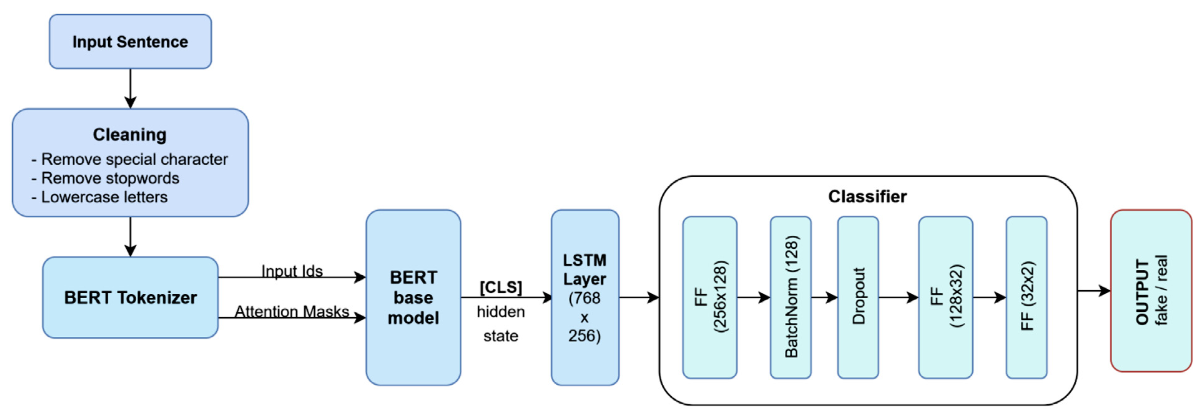
\includegraphics[scale=0.34]{static/bert_lstm_architecture.png}
    \caption{\label{fig:bert_lstm_architecture} Architekture des vorgeschlagenen hybriden Modells  \cite{RAI202298}}
    \end{center}
\end{figure}

Ziel des Papers ist es, die semantische Tiefe von BERT mit der temporalen Lernfähigkeit von LSTM zu verbinden, um Fake-News besser erkennen zu können.

Für die Evaluation wurde der FakeNewsNet-Datensatz verwendet. Dieser besteht aus dem PolitiFact- und dem GossipCop-Datensatz. 
PolitiFact enthält politisch orientierte Nachrichten, während GossipCop Nachrichten aus dem Unterhaltungsbereich beinhaltet. 
In beiden Datensätzen sind die Inhalte kategorisiert in echte und gefälschte Nachrichten. 
Die Datensätze bestehen aus Nachrichtentiteln. PolitiFact umfasst 432 falsche und 624 echte Titel, GossipCop 5323 falsche und 16.817 echte Titel.

\begin{figure}[htbp]
    \begin{center}
    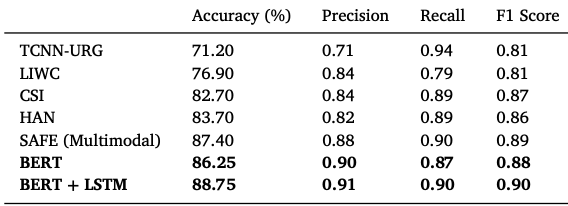
\includegraphics[scale=0.5]{static/bert_lstm_politifact.png}
    \caption{\label{fig:bert_lstm_politifact} Ergebnisse der verschiedenen Modelle mit dem PolitiFact Datensatz \cite{RAI202298}}
    \end{center}
\end{figure}

Das vorgeschlagene Modell, übertrifft klassische Methoden und auch reines BERT in der Fake-News-Erkennung. 
Auf dem PolitiFact-Datensatz erreicht es 88,75\% Genauigkeit (siehe Abbildung \ref{fig:bert_lstm_politifact}, bei reinem BERT sind es nur 86,25\%.
Der LSTM-Layer verbessert dabei die Nutzung der kontextuellen BERT-Embeddings, insbesondere bei der Analyse sprachlicher Muster in Newstiteln.

\subsection{BERT und BiLSTM}

\cite{wang2021covid19fakenewsdetection} stellt ein hybrides BERT und BiLSTM Modell vor. Hierbei wird ein vortrainiertes BERT-Modell als 
Merkmalsencoder genutzt. Dabei bleiben alle internen Gewichte und Parameter von BERT unverändert und werden nicht weiter trainiert. 
Zusätzlich wird ein BiLSTM Modell für die weitere Verarbeitung der BERT-Ausgaben trainiert (siehe Abbildung \ref{fig:bert_bilstm_architecture}).

\begin{figure}[htbp]
    \begin{center}
        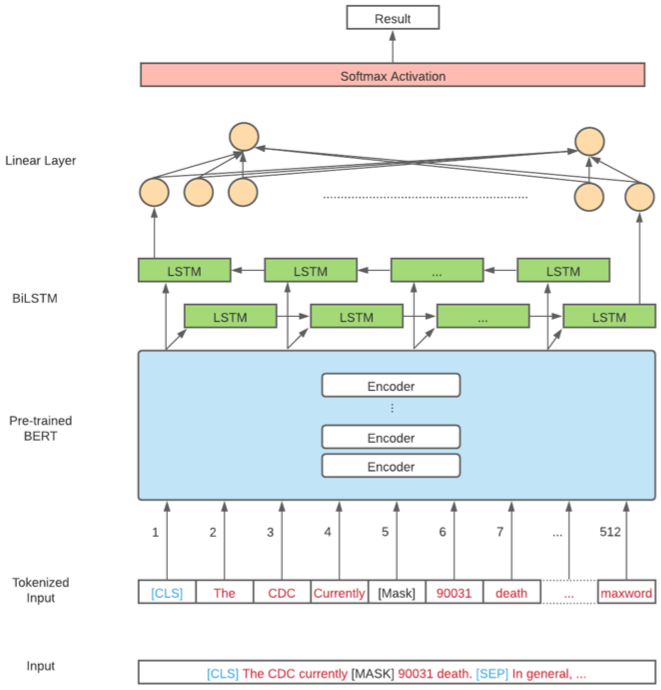
\includegraphics[scale=0.45]{static/bert_bilstm_architecture.png}
        \caption{\label{fig:bert_bilstm_architecture} Architektur des hybriden Modells \cite{wang2021covid19fakenewsdetection}}
    \end{center}
\end{figure}

Verwendet wurde ein COVID-19 Fake News Dataset von Kaggle, bestehend aus 6.420 Trainings- und 2.140 Testeinträgen. 
Jeder Eintrag enthält die Merkmale Tweet-ID, den Text des Tweets und ein Label (echt oder gefälscht).
Augrund der Größe dieses Datensatzes werden die internen Gewichte und Parameter von BERT nicht weiter trainiert.
Durch die etwa 8.500 Einträge ist der COVID-19-Datensatz zu klein, um das BERT-Modell effektiv und ohne Overfitting neu zu trainieren.
Durch das Einfrieren wird verhindert, dass die vortrainierten Sprachmuster überschrieben werden. 
So bleibt die allgemeine Sprachkompetenz von BERT erhalten, während das darauf aufbauende BiLSTM lernt, 
diese Informationen für die Fake-News-Erkennung zu nutzen.

Verglichen wurde von \cite{wang2021covid19fakenewsdetection} folgende Modelle:
\begin{itemize}
    \item \textbf{Modell 1:} Feinjustiertes BERT-Modell (ohne zusätzliche Schichten)
    \item \textbf{Modell 2:} BERT mit eingefrorenen Parametern + CNN-Schichten
    \item \textbf{Modell 3:} BERT mit nicht eingefrorenen Parametern + CNN-Schichten
    \item \textbf{Modell 4:} BERT mit eingefrorenen Parametern + BiLSTM-Schichten
    \item \textbf{Modell 5:} BERT mit nicht eingefrorenen Parametern + BiLSTM-Schichten
\end{itemize}

\begin{figure}[htbp]
    \begin{center}
    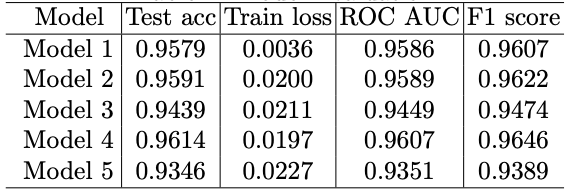
\includegraphics[scale=0.4]{static/bert_bilstm_results.png}
    \caption{\label{fig:bert_bilstm_results} Ergebnisse der verschiedenen Modelle \cite{wang2021covid19fakenewsdetection}}
    \end{center}
\end{figure}

Wie in Abbildung \ref{fig:bert_bilstm_results} zu sehen, hat das Modell 4 mit einer Test Accuracy von 96,14\% und einem F1-Score von 96,46\%
das beste Ergebnis.
Die Kombination aus dem beiden BERT und BiLSTM-Schichten liefert folglich den besten Ansatz zur COVID-19-Fake-News-Erkennung. 
Die Ergebnisse zeigen, dass sich die semantische Tiefe von BERT und sequentielle Kontextverarbeitung von BiLSTM gut ergänzen.

\subsection{BERT und LightGBM}
\label{sec:bert_lightgbm}

\cite{Essa:2023aa} entwickelte ein weiteres hybrides Modell welches das BERT-Embedding und ein LightGBM Modell nutzt.
Das Modell kombiniert die tiefen semantischen Sprachmerkmale von BERT mit der schnellen, skalierbaren Klassifikationsfähigkeit von LightGBM.
Im vorgestellten hybriden Modell wird die Eingabe mittels BERT verarbeitet (siehe Abbildung \ref{fig:bert_lightgbt_architecture}). 
Dabei wird der [CLS]-Token aus den letzten drei Encoderschichten extrahiert und zu einem einzigen Merkmalsvektor zusammengeführt. 
Dieser Vektor dient als Eingabe für LightGBM, das eine binäre Klassifikation in „wahr“ oder „falsch“ vornimmt.

\begin{figure}[htbp]
    \begin{center}
    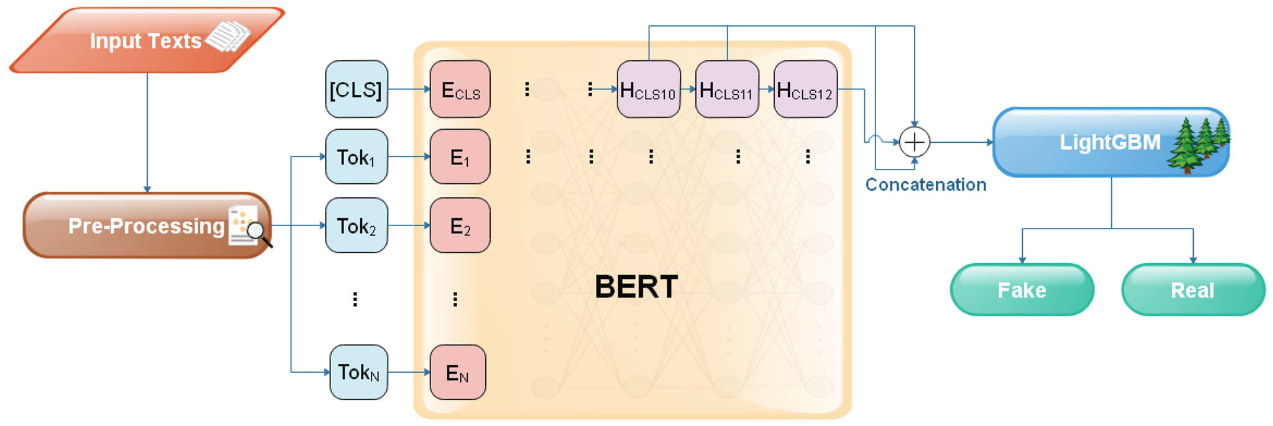
\includegraphics[scale=0.32]{static/bert_lightgbt_architecture.png}
    \caption{\label{fig:bert_lightgbt_architecture} Architektur des hybriden Modells \cite{Essa:2023aa}}
    \end{center}
\end{figure}

Genutzt werden in dem Paper folgende drei Datensätze:
\begin{itemize}
  \item \textbf{ISOT}: Enthält ca. 45.000 Artikel, gleichmäßig auf echte und gefälschte Nachrichten verteilt. 
  Die echten Artikel stammen von Reuters, die gefälschten von fragwürdigen Quellen laut PolitiFact. 
  Themenschwerpunkte sind Politik und Weltgeschehen (2016–2017).

  \item \textbf{TI-CNN}: Besteht aus 20.015 Artikeln (8074 echt, 11.941 falsch). Die echten Nachrichten stammen von renommierten Medien 
  wie der New York Times, die gefälschten von über 240 inoffiziellen Webseiten.

  \item \textbf{FNC (Fake News Corpus)}: Umfasst Millionen Artikel von über 1000 Domains. Für die Experimente wurde ein ausgeglichener 
  Datensatz aus je 500.000 echten und gefälschten Artikeln erstellt. Enthält zusätzliche Metadaten wie Titel, Autor und URL.
\end{itemize}

\begin{figure}[htbp]
    \begin{center}
    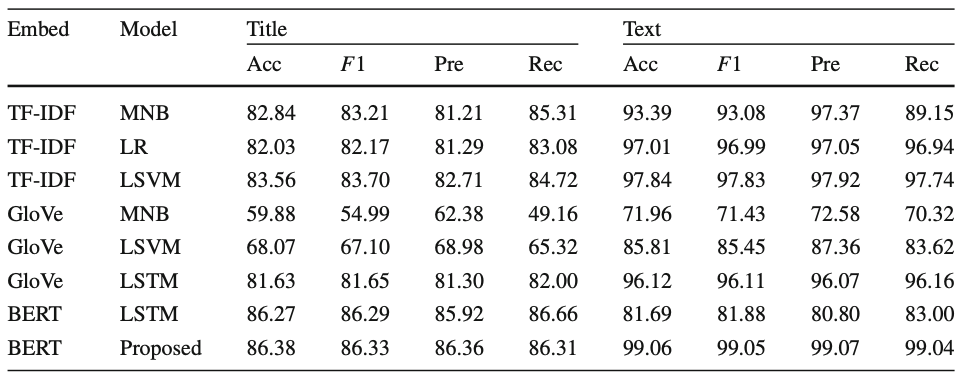
\includegraphics[scale=0.4]{static/bert_lightgbt_results.png}
    \caption{\label{fig:bert_lightgbt_results} Ergebnisse der verschiedenen Modelle auf dem FNC-Datensatz \cite{Essa:2023aa}}
    \end{center}
\end{figure}

In Abbildung \ref{fig:bert_lightgbt_results} zu sehen ist, dass dieses Modell anderen gerade bei großen Datenmengen überlegen ist.
\cite{Dhiman:2024aa} nennt dieses Modell im August 2024 mit einer Accuracy von 99,06\% die beste State-of-the-Art-Technik.


\subsection{RoBERTa und LightGBM}
\label{sec:roberta_lightgbm}

%TODO: schreiben

Aufbauend auf dem hybriden BERT und LightGBM Model zeigt \cite{V_G_2024} die Vorteile eines hybriden RoBERTa-LightGBM Modells.

RoBERTa ist eine weiterentwickelte und leistungsstärkere Version von BERT, die durch effizienteres Training und größere Datenbasis 
bessere Ergebnisse in der Fake-News-Erkennung erzielt. 
Statt mit den 16GB Textdaten des BERT Modells wurde RoBERTa mit über 160GB trainiert, wodurch eine deutlich bessere Generalisierungsfähigkeit besteht.
Außerdem nutzt RoBERTa nicht mehr das statische maskieren (MLM) wie BERT, sondern ein fortgeschritteneres dynamisches maskieren.
Hierbei wird jedes mal genau dann ein Maskierungspattern generiert, wenn eine Sequenz einem Modell hinzugefügt wird \cite{roberta:main}.

Das Paper verwendet den „Fake News Detection Dataset“ zum Training. 
Die Daten stammen von reuters.com und umfassen jeweils 12.600 Artikel, gesammelt in den Jahren 2016 bis 2017.

Nach der Vorverarbeitung wurden die Daten tokenisiert und mit Roberta in Vektor-Embeddings umgewandelt.
Verwendet wird der [CLS] Token aus den letzten drei Hidden Layers, um den gesamten Text zu repräsentieren.
Durch Self Attention liefert dies eine feste, dichte Vektor-Repräsentation pro Artikel.
Diese Embeddings dienten anschließend als Eingabe für LightGBM zur binären Klassifikation.

RoBERTa-LightGBM erzielt eine Verbesserung gegenüber BERT-LightGBM von bis zu 21\% (siehe Abbildung \ref{fig:roberta_lightgbm_auc_roc_value}).

\begin{figure}[htbp]
    \begin{center}
    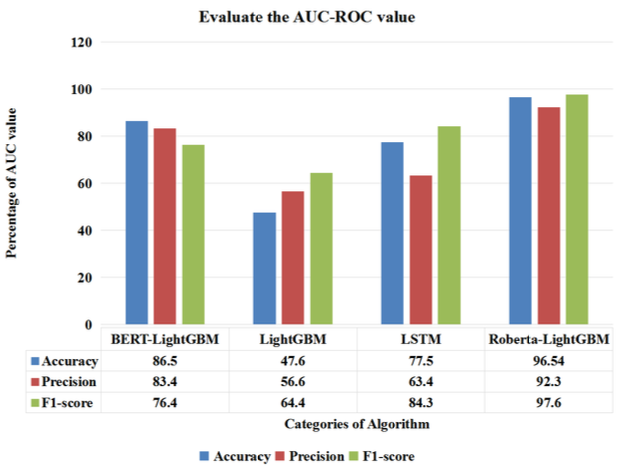
\includegraphics[scale=0.5]{static/roberta_lightgbm_auc_roc_value.png}
    \caption{\label{fig:roberta_lightgbm_auc_roc_value} Auswertung der verschiedenen AUC ROC Werte \cite{V_G_2024}}
    \end{center}
\end{figure}
\chapter{Relevante Datensätze und Auswahlkriterien}
\label{chap:relevante_datensaetze_und_auswahlkriterien}

\section{Vorstellung verfügbarer deutscher Fake-News-Datensätze}
\label{sec:vorstellung_verfuegbare_deutsche_fake_news_datensaetze}

\begin{table}[ht]
    \centering
    \renewcommand{\arraystretch}{1.3}
    \begin{tabular}{|p{1.9cm}|p{2.3cm}|p{1.3cm}|p{1.3cm}|p{3.3cm}|p{1.5cm}|}
        \hline
        \textbf{Datensatz} & \textbf{Quelle} & \textbf{Anzahl Zeilen} & \textbf{Anteil Fake (\%)} & \textbf{Besonderheiten / Einschränkungen} & \textbf{Eignung} \\
        \hline
        \textbf{Fake News Dataset German} & University of Applied Sciences Upper Austria & 63.868 & 7{,}24\,\% & Geringer Anteil an Fake-News $\rightarrow$ unausgewogene Klassenverteilung & Weniger geeignet \\
        \hline
        \textbf{German-Fake NC} & Fraunhofer-Institut für Sichere Informationstechnologie SIT & 489 & 100\,\% & Enthält nur Referenzen, keine Texte $\rightarrow$ keine direkte Textauswertung möglich & Nicht geeignet \\
        \hline
        \textbf{FANG-COVID} & Association for Computational Linguistics & 41.242 & 31{,}97\,\% & Ausgewogene Klassen, vollständige Texte, viele Metadaten (Titel, Header, Label) & \textbf{Sehr geeignet} \\
        \hline
        \textbf{DeFaktS} & FZI Forschungszentrum Informatik & -- & -- & Kein Zugang $\rightarrow$ Nutzung ausgeschlossen & Nicht verfügbar \\
        \hline
    \end{tabular}
    \caption{Vergleich deutscher Fake-News-Datensätze}
    \label{tab:deutsche-fake-news-datensaetze}
\end{table}

In der Tabelle \ref{tab:deutsche-fake-news-datensaetze} sind verschiedene deutsche Fake-News-Datensätze gelistet.
Die Eignung bezieht sich darauf, wie sinnvoll die Nutzung dieser jeweiligen Datensätze für das Trainieren eines Modells zum Erkennen von Fake News ist.

%TODO: kurze beschreibung für jeden datensatz 

\section{Nutzung englischer Datensätze}

Eine in \cite{Simone2022} angewandte Lösung ist die Erstellung eines großen Datensatzes mit englischen Artikeln. Das Modell wurde entsprechend auf Englisch 
trainiert und die deutschen Artikel in der späteren Anwendung vor der Vorhersage übersetzt.
Fake News haben oft stilistische, semantische oder rhetorisch manipulierende Muster, welche sich je nach Sprache unterscheiden können.
Selbst mit modernen Transformern können diese Muster nicht sicher mit übersetzt werden, da diese einen übersetzen Artikel einer anderen Domäne zuordnen könnten
als den ursprünglichen Artikel \cite{hong2023disentanglingstructurestylepolitical}. 
Ein typisches Beispiel ist der Satz: „Natürlich wird das RKI bald neue Lockdowns empfehlen – die haben ja auch sonst nichts zu tun.“ 
Die Übersetzung ins Englische („Of course, the RKI will soon recommend new lockdowns – they have nothing else to do anyway“) wirkt sprachlich korrekt, 
verliert jedoch die ironisch-sarkastische Eigenschaft.
Das Ergebnis ist eine eher sachliche Aussage, welche vom englischen Modell sehr wahrscheinlich nicht mehr als Fake-News klassifiziert wird.
Solche stilistischen Abschwächungen sind ein Merkmal von maschinellen Übersetzungen, was sie in diesem Fall problematisch
für den Einsatz in der Fake-News-Erkennung macht \cite{kuehn2024enhancingrhetoricalfigureannotation}. %TODO: ChatGPT Beispiel

\section{Auswahl und Begründung des finalen Datensatzes}
\label{sec:auswahl_und_begruendung_finaler_datensatz}

Da der DeFaktS Datensatz nicht öffentlich verfügbar ist fällt dieser aus der Auswahl. 
Um ein Modell zu trainierien werden viele Daten benötigt. Im Kapitel \ref{sec:bert_lightgbm} umfassen die Datensätze von 20.000 bis hin zu Millionen Artikeln.
Deshalb entfällt auch der GermanFakeNC Datensatz.

Ein Problem, dass der Fake News Dataset German Datensatz (FNDG) bringt, ist die stark unausgewogene Klassenverteilung. Nur 7,24\% der 64.868 Einträge sind 
als Fake-News gekennzeichnet. Dadurch kann es beim Trainieren eines Modells dazu kommen, dass es überwiegend die häufiger vorkommenen echten Artikel 
lernt und Fake-News kaum oder gar nicht erkennt. 
Ein Modell könnte beispielsweise stets „echt“ vorhersagen und damit auf diesem Datensatz eine hohe Accuracy erreichen.
Bei späterer Anwendung würde es aber die entscheidenden Fälle nicht mehr differenzieren können. 
Das führt zu einem guten Accuracy-Wert, während Recall und F1-Score für die Fake-Klasse deutlich leiden. 
Das Modell verfehlt somit genau die Einträge, die für die Anwendung zentral sind.
Inhaltlich sind die Einträge aber auf einem breiten Gebiet verteilt, was einen Teil dieses Datensatzes für die Auswahl interessant macht.

Der verbleibende FANG-COVID Datensatz \cite{mattern-etal-2021-fang} fällt aufgrund seiner vielen Einträge und guter Klassenausgewogenheit
in die engere Auswahl. Problematisch bei diesem Datensatz ist aber, dass sich alle Einträge im COVID-19 Pandemie Kontext befinden.
Es besteht die Gefahr einer thematischen Überanpassung. Das Modell lernt vor allem, typische Begriffe, Erzählmuster und 
Formulierungen im Zusammenhang mit Pandemie-Fake-News zu erkennen. Dazu können zum Beispiel Impfgegner-Rhetorik, Verschwörungen oder auch Begriffe 
wie „PCR-Test“, „Lockdown“ oder „RKI“ gehören. In anderen Themenbereichen wie Politik, Migration oder Klima erkennt es dagegen manipulierte Inhalte 
unter Umständen nicht, da es diese Muster nie gelernt hat.
Außerdem kann das Modell semantische Verzerrungen entwickeln. Wörter, die in Pandemie-Fake-News häufig auftreten, könnten fälschlich als 
Indiz für eine Fake Klassifierung gewertet werden, auch wenn sie in neutralem oder echtem Kontext auftreten \cite{chen2023, nan2022improvingfakenewsdetection}. 
Dadurch steigt die Gefahr von False Positives bei echten Nachrichten außerhalb des COVID-Kontexts.
Ein Modell, das nur mit COVID-bezogenen Daten trainiert wurde, kann inhaltlich und stilistisch stark eingeschränkt generalisieren und 
verfehlt damit das Ziel, Fake News themenübergreifend zuverlässig zu erkennen.

Durch die Analyse der Datensätze ergeben sich folgende Möglichkeiten für das Trainieren eines Modells zur Fake-News Erkennung:
\begin{itemize}
    \item Nur FANG-COVID mit allen 41.242 Einträgen, aber 31,97\% Klassenausgewogenheit
    \item FANG-COVID mit ca. 26.000 Einträgen aber dafür 50/50 Klassenausgewogenheit
    \item FANG-COVID und FNDG kombiniert für bessere Generalisierung (105.110 Einträge, aber 16,94\% Klassenausgewogenheit)
    \item FANG-COVID und alle Fake Artikel von FNDG kombiniert für bessere Klassenausgewogenheit und mehr Daten
    (45.866 Einträge mit 38.82\% Klassenausgewogenheit)
    \item Alle Fake Einträge aus FANG-COVID und FNDG kombiniert (17.809 Fake Einträge) kombiniert mit Stichproben aus sowohl FANG-COVID als auch FNDG
    um eine sinnvolle Klassenausgewogenheit mit vielen Daten und einer guten Generalisierung zu erreichen (45.866 Einträge mit 38.82\% Klassenausgewogenheit,
    aber 28.057 echten Einträgen zu 50/50 aus FANG-COVID und FNDG).
\end{itemize}
\chapter{Konzeption der Softwarelösung}
\label{chap:konzeption_der_softwareloesung}

\section{Konzeption des Machine Learning Modells} \label{sec:06:machine_learning_model}

\subsection{Auswahl und Begründung der genutzten Modelle} 

Um ein Modell zu entwickeln, welches möglichst gute Metriken erzielt, müssen verschiedenen Modelkombinationen getesten werden.
Basierend auf den Arbeiten von \cite{Essa:2023aa} und \cite{V_G_2024}, welche Accuracy Werte bis zu 99,06\% erreichten, werden in dieser Arbeit weitere BERT und RoBERTa
Modelle mit LightGBM kombiniert.

Der wesentliche Vorteil beim Kombinieren der Transformer Modelle mit dem LightGBM Modell liegt in den verschiedenen Stärken der beiden Ansätze:

Transformer Modelle wie BERT, bzw. RoBERTa extrahieren Sprachrepräsentationen und erfassen dabei den Kontext
eines Wortes im Satz, indem sie sowohl den vorhergehenden als auch den nachfolgenden Text berücksichtigen.
Dabei wird der vollständige sprachliche Zusammenhang eines Tokens innerhalb des gesamten Satzes oder Dokuments erkannt.

Im Gegensatz dazu ist LightGBM ein leistungsstarker, baumbasierter Klassifikator. Die Stärken dieses Modells liegen in Effizienz, Skalierbarkeit und Robustheit.
Es arbeitet besonders gut bei tabellarischen, hochdimensionalen Feature-Repräsentationen. 
Diese können zum Beispiel durch BERT-Embeddings entstehen.
Außerdem erfolgt die finale Klassifikation über LightGBM mit deutlich weniger Rechenaufwand, da keine weitere tiefere neuronale Architektur benötigt wird.

Beide Arbeiten zeigen, dass die Kombination zu besserer Generalisierung, niedrigerem Overfitting und schnellerem Training führt.

Folgende Kombinationen werden im Folgenden verglichen:
\begin{itemize}
    \item BERT und LightGBM
    \item RoBERTa und LightGBM
    \item XML-RoBERTa und LightGBM
\end{itemize}

\subsection{Datenvorverarbeitung} \label{sec6:datenvorverarbeitung}

Der FNDG Datensatz enthält die Merkmale 'id', 'url', 'Titel', 'Body', 'Kategorie', 'Datum', 'Quelle', 'Fake' und 'Art'.
Hiervon beinhalten die drei Merkmale 'Titel', 'Body' und 'Fake' die relevanten Informationen für diese Anwendung.
In 'Titel' steht die jeweilige Überschrift des Artikels und in 'Body' der eigentliche Inhalt. Das Merkmal 'Fake' gibt in der Nominalskala
an ob der Artikel als gefälscht klassifiziert ist oder nicht (1 für Fake, 0 für echt).

Im FANG-COVID Datensatz sind die Merkmale 'Unnamed: 0.1', 'Unnamed: 0', 'article', 'date', 'header', 'label', 'url', 'hist', 'tweeet', 'repl', 'retw', 'like' und 'quote'
enthalten. 'article', 'header' und 'label' sind hierbei relevant. 'header' und 'article' sind analog zum FNDG Datensatz Überschrift und Inhalt
des Artikels. 'label' enthält entweder den Wert 'real' um den Artikel als echt oder 'fake' um den Artikel als gefälscht zu klassifizieren.

Die beiden Datensatze werden zur Weiterverarbeitung zusammengefasst. Überschrift und Inhalt werden konkateniert, da das RoBERTa Modell nur
einen Wert pro Label verarbeiten kann. Dieses Merkmal wird umbenannt zu 'text'. 
Für die Klassifizierungskennzeichnung wird die Nominalskala des FNDG Datensatzes und der Titel des FANG-Covid Datensatzes übernommen.

Der finale Datensatz umfasst 45869 Artikel mit jeweils dessen \textit{text} und \textit{label}.
38,83\% dieser Artikel (17.813) sind Fake. 

Die Aufteilung der Daten erfolgt in Trainings-, Validierungs- und Testdatensätze. 
80\% des Gesamtdatensatzes werden für das Training genutzt und jeweils 10\% für das Validierung und Testen.

\subsection{Fine-tuning der Transfomer Modelle}

Transformer Modelle wie zum Beispiel BERT sind in der Regel vortrainiert. Dabei werden sie auf großen Mengen unannotierter Textdaten trainiert, um ein allgemeines Sprachverständnis 
zu erlernen. Dieser gesamte Prozess erfolgt unüberwacht.
Um die vortrainierten Transformer Modelle für die Fake-News Erkennung nutzbar zu machen, müssen sie einmalig an die spezifische Aufgabe angepasst werden (\textit{Fine-Tuning}).
Hierfür wird das Modell auf dem in Kapitel \ref{sec6:datenvorverarbeitung} erzeugtem Datensatz weitertrainiert. Dabei wird die zugrundeliegenden Sprachrepräsentationen auf 
die konkrete Zielaufgabe, der Fake-News Klassifizierung übertragen.

\subsection{Erzeugung der Embeddings}

Nach der Aufteilung des Datensatzes, werden diese Daten von den Transformer Modellen in Embeddings umgewandelt.
Zuerst werden die Eingaben dafür in Token zerlegt.
BERT nutzt den WordPiece Tokenizer, RoBERTa das Byte-Pair-Encoding und XML-RoBERTa den SentencePiece Tokenizer.
Alle diese Tokenizer zerteilen Wörter unterschiedlich, was zu verschiedenen Tokenfolgen und damit auch zu unterschiedlichen Embedding-Repräsentationen führt.

Eine wichtige Eigenschaft der drei Transformer Modelle ist, dass nach dem Tokenisieren maximal 512 Token pro Eingabe verarbeitet werden können.
Was genau ein Token ist, hängt in diesem Fall vom genutzten Tokenizer ab. Es kann sowohl ein Wort als auch nur ein Wortfragment sein.
Alle Token einer zu verarbeitenden Eingabe, die nach dem 512. Token kommen, werden abgeschnitten.
Eingabesequenzen, welche kürzer als 512 Token sind, werden mit angehängten \texttt{[PAD]}-Tokens aufgefüllt, damit alle Eingaben die gleiche Länge haben.

\cite{sun2020finetuneberttextclassification} testet verschiedene \textit{Truncation}-Methoden und zeigt für BERT, dass bei Filmrezensionen und Nachrichtenartikeln eine 
Zusammensetzung der ersten 256 und letzten 256 Token am effektivstem ist. Der Unterschied zur Nutzung der ersten 512 Token ist aber minimal, daher wird in dieser Arbeit letzteres
implementiert.

Die erzeugten Token werden von den jeweiligen angepassten Transformer Modellen in dichte Vektoren verarbeitet.
Diese Vektoren bilden die Grundlage für die nachfolgenden \textit{Self-Attention}-Mechanismen, die kontextabhängige, semantisch reichhaltige Embeddings erzeugen.
Diese Embeddings entstehen über mehrere aufeinanderfolgende \textit{hidden layers}, wobei jede Schicht die Werte weiter verfeinert und anreichert.

Um die Ausgabe der verschiedenen Embeddings der \textit{hidden layer} zusammenzufassen kann zum Beispiel der \texttt{[CLS]}-Token aus einer oder mehreren Schichten extrahiert oder 
ein Durchschnitt aller Token-Embeddings gebildet werden.

\cite{sun2020finetuneberttextclassification} zeigt für BERT, dass die letzten Layer die meisten Informationen beinhalten.
In dieser Arbeit wird aus den letzten vier Layern ein Durchschnittswert gebildet.

\subsection{Nutzung der Embeddings im LightGBM Modell}

Der für das Trainieren des LightGBM Modells benötigte Datensatz setzt sich aus der jeweiligen Zusammenfassung der \textit{hidden layer} und dem Klassifizierungslabel 
des Artikels, durch welches die Embeddings erzeugt wurden, zusammen. 

Für das Training werden die Artikel des in Kapitel \ref{sec6:datenvorverarbeitung} erzeugten Datensatzes gemappt. 
Jeder Artikel wird hierbei durch ein, vom angepassten Transformer Modell erzeugten zusammengefassten Embedding ersetzt.
Das entsprechende Label wird als zweite Spalte ergänzt.

Das trainierte LightGBM Modell kann anschließend neu erzeugte Embeddings effizient klassifizieren.

\subsection{Gesamtarchitektur}

Für die finale Anwendung dieser Arbeit wird ein Webserver aufgesetzt, welcher Nachrichtenartikel empfängt und diese anhand der konfigurierten Modelle tokenisiert, eingebettet und
klassifiziert (siehe Abbildung \ref{fig:beispielablauf_gesamt}).

\begin{figure}[htbp]
    \begin{center}
        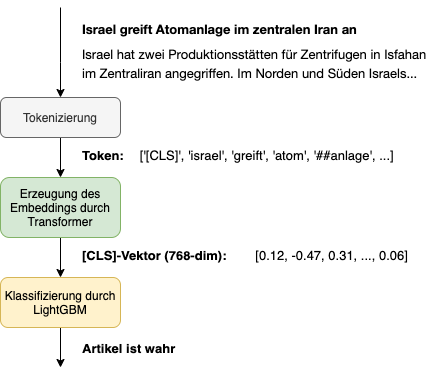
\includegraphics[scale=0.6]{diagrams/beispielablauf_gesamt.png}
        \caption{\label{fig:beispielablauf_gesamt} Beispielhafter Ablauf einer Klassifizierung eines Artikels}
    \end{center}
\end{figure}

\section{Konzeption des Webagenten} \label{sec:06:hauptkomponente}

Der Webagent hat die Aufgabe die Artikel auf den verschiedenen Nachrichtenportalen zu lesen und zu ergänzen.
Hierfür muss erkannt werden auf welcher Seite sich der Nutzer befindet. Außerdem muss das html dieser Seite ausgelesen und analysiert werden können.

\paragraph{Als Beispiel die Seite Bild.de:} 
Je nach Fenstergröße hat die Seite entweder die Domäne \textit{https://www.bild.de/} oder \textit{https://m.bild.de/}.

Die Startseite ist wie folgt aufgebaut:

\begin{lstlisting} [language=html]
    <!DOCTYPE html>
    <html>
      <head>
        ...
      </head>
      <body>
        <div id="app">
            ...
            <div id="page-content">
                <header/>
                    <main>
                    <!-- Es gibt auf der Startseite 
                    ueber 50 dieser section-Elemente -->
                        <section>
                            <article/>
                        </section>
                    </main>
                <footer/>
            </div>    
        </div>
      </body>
    </html>
\end{lstlisting}

Wenn ein Artikel geöffnet ist, ist der DOM dem der Startseite sehr ähnlich. Der einzige wesentliche Unterschied ist, dass im \textit{main}-Element
nur noch ein \textit{article}-Element ist und nicht beliebig viele \textit{section}-Elemente.
Ob ein Artikel geöffnet ist, kann also anhand der Anzahl der \textit{article}-Elemente bestimmt werden.

\begin{lstlisting} [language=html]
    <article>
        <h2 class="document-title document-title-article">
            <span class="kicker">Kicker des Artikels</span>
            <span class="headline">Titel des Artikels</span>
        </h2>
    </article>
    <div class="article-body">
        <!-- Pro Artikel gibt es ca. 10 p-Elemente -->
        <p>Inhalt des Artikels</p>
    </div>
\end{lstlisting}

Der Titel und Inhalt des Artikels kann den entsprechenden html-Elementen entnommen werden.
Diese werden anschließend an die API gesendet und dort verarbeitet. 
Der Rückgabewert der API enthält dann die Info ob der Artikel falsch oder echt ist.
Diese wird in einem vom Webagent erzeugten \textit{div}-Container über dem Artikel eingefügt.

%TODO: nicht eher umsetzung?
Zur Bestimmung des geeignetsten Tools für diese Anforderungen,
wurden verschiedene Technologien verglichen (siehe Tabelle \ref{table:technischeAnsaetze}).
Aufgrund des begrenzten Zugriffs auf die zu analysierende Seiten, bieten sich die beiden Client-seitigen Umsetzungen 
eine Chrome Extension zu implementieren oder über Tampermonkey Userscripts auszuführen am ehesten an.

Im Vergleich zu Usercripts unterstützt die Extension mehrere Komponenten (Content Scripts, Background Scripts, Popup, Optionsseite).
Anhand dieser können der DOM beobachtet, ein persistenter Speicher genutzt, Kontextmenüs erstellt und auf Browseraktionen reagiert werden (z.B. Tabwechsel, Navigation).
Ein Userscript hingegen ist ein einfaches Script, das nur beim Laden einer Seite aktiv ist und dementsprechend keine Hintergrundverarbeitung und keine erweiterten UI-Komponenten
zur Verfügung stellt.

Zur Implementierung des Webagents wird also eine Chrome Extension genutzt.

    
    
    
\chapter{Umsetzung des Prototyps}
\label{chap:umsetzung_des_prototyps}

\section{Implementierung des Machine Learning Modells}

In \ref{tab:bert_models} angehängt, findet sich ein tabellarischer Vergleich der verschiedenen BERT- und RoBERTa-Modelle.


\section{Implementierung der Chrome Erweiterung}

Die Chrome Erweiterung wurde mit der Version Manifest 3 implementiert.
Genutzt wurden ein \textit{Service Worker} ein \textit{Content Script} pro Nachrichtenportal und ein \textit{Popup}.

\paragraph{Service Worker} steuern eine Seite genau dann, wenn ein Service Worker auf dieser Netzwerkanfragen in seinem Namen abfangen kann. 
Der Service Worker kann dann Aufgaben für die Seite innerhalb eines bestimmten Scopes ausführen

Der Lifecycle eines Service Workers ist in folgende Events unterteilt: installing, installed, activating, activated.

Nach Abschluss der Aktivierung steuert der Service Worker die Seite standardmäßig erst 
bei der nächsten Navigation oder Seitenaktualisierung \cite{chrome2025serviceworker}.

\paragraph{Content Scripts} sind Dateien, die im Kontext von Webseiten ausgeführt werden. 
Mit dem standardmäßigen Document Object Model (DOM) können sie Details der Webseiten lesen, die der Browser besucht, 
Änderungen daran vornehmen und Informationen an die übergeordnete Erweiterung weitergeben \cite{chrome2025contentscripts}.

Die Kommunikation mit den Service Worker erfolgt über die Extension-API \textit{runtime}.

\paragraph{Pop-ups} sind Aktionen, bei denen ein Fenster angezeigt wird, über das Nutzer mehrere Erweiterungsfunktionen aufrufen kann. 
Sie werden durch ein Tastenkürzel, durch Klicken auf das Aktionssymbol der Erweiterung oder durch Drücken von chrome.action.openPopup() ausgelöst. 
Pop-ups werden automatisch geschlossen, wenn der Nutzer sich auf einen Bereich des Browsers außerhalb des Pop-ups konzentriert \cite{chrome2025popups}.

In Abbildung \ref{fig:seq_hauptkomponente} zu sehen ist das Sequenzdiagramm des Webagents. Wie in Kapitel \ref{sec:06:hauptkomponente} beschrieben
wird zuerst die URL geprüft. Erfüllt diese die vorgegebenen Bedingungen wird der geöffnete Artikel gelesen und von einer weiteren Anwendung
analysiert. Anschließend wird das Ergebnis der Analyse in einem \textit{div}-Container über dem Artikel eingefügt.

Um die Veränderungen im Browser zu überwachen wurde die \textit{tabs}-API von Chrome genutzt. Anhand dieser kann das Tab-System eines Browsers überwacht
und zum Beispiel auch auf jede Veränderung der URL reagiert werden.
Außerdem ermöglicht die API das Versenden von Nachrichten an alle aktiven Content Scripts. Diese werden dann im jeweiligen Content Script über die
\textit{runtime}-API empfangen und ausgelesen.



\chapter{Evaluation und Ergebnisse}
\label{chap:evaluation_und_ergebnisse}

\section{Leistungs-Analyse der Transformer- und LightGBM-Modelle}

Tabelle \ref{tab:overfitting_check} vergleicht die Accuracy- und F1-Werte der Trainings- und Testphase für alle fünf untersuchten Transformer-Modelle. 
Die zusätzlich angegebenen Differenzwerte ($\Delta$) zeigen den Unterschied zwischen Test- und Trainingsergebnissen. 
Da die Abweichungen in beiden Metriken bei allen Modellen sehr klein ist, lässt sich daraus schließen, dass kein Overfitting vorliegt. 
Die Modelle generalisieren gut und zeigen eine stabile Leistung auf bislang ungesehenen Daten.

\begin{table}[ht]
\centering
\begin{tabular}{lcccccc}
    \toprule
    \multirow{2}{*}{Modell} & 
    \multicolumn{2}{c}{Training} & 
    \multicolumn{2}{c}{Test} & 
    \multicolumn{2}{c}{$\Delta$ (Test - Train)} \\
    \cmidrule(lr){2-3} \cmidrule(lr){4-5} \cmidrule(l){6-7}
    & Accuracy & F1 & Accuracy & F1 & $\Delta$ Acc & $\Delta$ F1 \\
    \midrule
    XLM-RoBERTa-Large   & 0.9780 & 0.9780 & 0.9795 & 0.9795 & +0.0015 & +0.0015 \\
    XLM-RoBERTa-Base    & 0.9730 & 0.9729 & 0.9717 & 0.9716 & $-$0.0013 & $-$0.0013 \\
    RoBERTa-Large       & 0.9795 & 0.9795 & 0.9765 & 0.9764 & $-$0.0030 & $-$0.0031 \\
    RoBERTa-Base        & 0.9771 & 0.9771 & 0.9751 & 0.9751 & $-$0.0020 & $-$0.0020 \\
    BERT-Base-Uncased   & 0.9507 & 0.9505 & 0.9533 & 0.9531 & +0.0026 & +0.0026 \\
    \bottomrule
\end{tabular}
\caption{Vergleich von Training und Test: Accuracy und F1 zur Überprüfung von Overfitting}
\label{tab:overfitting_check}
\end{table}

Tabelle \ref{tab:vergleich_der_transformer_modelle} zeigt die Testergebnisse der fünf untersuchten Transformer-Modelle nach dem Fine-Tuning auf dem 
Klassifikationsdatensatz. 
Dargestellt sind Accuracy, F1-Score, Loss sowie die durchschnittliche Evaluationszeit. Das Modell XLM-RoBERTa-Large erzielt mit einer 
Accuracy und einem F1-Score von jeweils 97,95\% die besten Resultate, gefolgt von RoBERTa-Large und RoBERTa-Base. 
Das schwächste Ergebnis liefert BERT-Base-Uncased mit einem Accuracy-Wert von 95,33\%. Insgesamt zeigt sich, dass die \textit{Large}-Varianten
der Tranformer Modelle bessere Ergebnisse erzielen, allerdings auch mit einem erhöhten Evaluationsaufwand verbunden sind.

\begin{table}[!ht]
\centering
\begin{tabular}{lcccc}
    \toprule
    \textbf{Modell} & \textbf{Accuracy} & \textbf{F1-Score} & \textbf{Loss} & \textbf{Eval-Zeit (s)} \\
    \midrule
    XLM-RoBERTa-Large & 0.9795 & 0.9795 & 0.1070 & 13.96 \\
    RoBERTa-Large     & 0.9765 & 0.9764 & 0.1395 & 14.04 \\
    RoBERTa-Base      & 0.9751 & 0.9751 & 0.1273 & 5.86 \\
    XLM-RoBERTa-Base  & 0.9717 & 0.9716 & 0.1527 & 5.77 \\
    BERT-Base-Uncased & 0.9533 & 0.9531 & 0.1952 & 6.33 \\
    \bottomrule
\end{tabular}
\caption{Testergebnisse der Transformer Modelle nach dem Fine-Tuning}
\label{tab:vergleich_der_transformer_modelle}
\end{table}

In Tabelle \ref{tab:vergleich_lightgbm_modelle} dargestellt, sind die Metriken verschiedener LightGBM-Modells, welche auf den neu erzeugten 
Embeddings der verschiedenen Transformer-Modellen trainiert wurden.
Dabei wurden jeweils die letzten vier Schichten der Modelle gemittelt und als Input für den LightGBM-Classifier verwendet. 
Auch in diesem Setup erzielt XLM-RoBERTa-Large mit einer Accuracy von 97,84\% und einem F1-Score von 97,73\% die besten Ergebnisse. 
Es folgen die \textit{Base}-Varianten von XLM-RoBERTa und RoBERTa mit sehr ähnlichen Werten. Deutlich schwächer schneidet BERT-Base-Uncased ab, 
was auf eine geringere Qualität der erzeugten Embeddings hinweist. Insgesamt zeigt sich, dass die Qualität der Repräsentationen der Transformer-Modelle 
einen wesentlichen Einfluss auf die nachgelagerte Klassifikationsleistung hat.

\begin{table}[!ht]
\centering
\begin{tabular}{lcc}
    \toprule
    \textbf{Embedding-Modell} & \textbf{Accuracy} & \textbf{F1-Score} \\
    \midrule
    XLM-RoBERTa-Large & 0.9784 & 0.9773 \\
    XLM-RoBERTa-Base  & 0.9753 & 0.9738 \\
    RoBERTa-Large     & 0.9753 & 0.9738 \\
    RoBERTa-Base      & 0.9729 & 0.9713 \\
    BERT-Base-Uncased & 0.9472 & 0.9439 \\
    \bottomrule
\end{tabular}
\caption{Testergebnisse der LightGBM-Modelle nach dem Training auf den Embeddings}
\label{tab:vergleich_lightgbm_modelle}
\end{table}

Tabelle \ref{tab:transformer_vs_lightgbm} vergleicht die Accuracy- und F1-Werte der Transformer und LightGBM Modelle.
Der Differenzwert ($\Delta$) zeigt den Unterschied zwischen den beiden Modellen.
Es zeigt sich, dass die direkt feinjustierten Transformer-Modelle in fast allen Fällen leicht bessere Ergebnisse erzielen als die Kombination aus 
Embeddings und LightGBM.

\begin{table}[!ht]
\centering
\begin{tabular}{lcccccc}
    \toprule
    \multirow{2}{*}{\textbf{Modell}} &
    \multicolumn{2}{c}{\textbf{Transformer}} &
    \multicolumn{2}{c}{\textbf{LightGBM}} &
    \multicolumn{2}{c}{$\Delta$ (LGBM - TF)} \\
    \cmidrule(lr){2-3} \cmidrule(lr){4-5} \cmidrule(l){6-7}
    & \textbf{Accuracy} & \textbf{F1} & \textbf{Accuracy} & \textbf{F1} & $\Delta$ Acc & $\Delta$ F1 \\
    \midrule
    XLM-RoBERTa-Large & 0.9795 & 0.9795 & 0.9784 & 0.9773 & $-$0.0011 & $-$0.0022 \\
    RoBERTa-Large     & 0.9765 & 0.9764 & 0.9753 & 0.9738 & $-$0.0012 & $-$0.0026 \\
    RoBERTa-Base      & 0.9751 & 0.9751 & 0.9729 & 0.9713 & $-$0.0022 & $-$0.0038 \\
    XLM-RoBERTa-Base  & 0.9717 & 0.9716 & 0.9753 & 0.9738 & +0.0036 & +0.0022 \\
    BERT-Base-Uncased & 0.9533 & 0.9531 & 0.9472 & 0.9439 & $-$0.0061 & $-$0.0092 \\
    \bottomrule
\end{tabular}
\caption{Vergleich von Transformer- und LightGBM-Modellen: Accuracy, F1 und Differenz}
\label{tab:transformer_vs_lightgbm}
\end{table}

Ein möglicher Grund für die leicht schlechteren Metriken bei der Verwendung von LightGBM könnte in der hohen semantischen Dichte und Dimension der 
Transformer-Embeddings liegen. Diese enthalten sehr viele komplexe, kontextuelle Informationen, die zwar für überwachte Modelle direkt nutzbar sind, 
klassische Modelle wie LightGBM jedoch nur eingeschränkt verarbeiten können.
\cite{reimers-gurevych-2019-sentence} erklärt, dass die Architektur von BERT für die Anwendung in weiteren unüberwachte Verfahren problematisch ist.
Es lässt sich vermuten, dass Gleiches auch für überwachte Modelle gilt.

\section{Vergleich mit verwandten Arbeiten}

Tabelle \ref{tab:vergleich_literatur} vergleicht die Accuracy- und F1-Scores der in dieser Arbeit entwickelten Modelle mit den besten Resultaten zweier 
verwandter Studien. Während \cite{Essa:2023aa} ihre Modelle auf drei unterschiedlichen Fake-News-Datensätzen getestet hat 
(ISOT, TI-CNN, FNC), stammen die Ergebnisse aus \cite{V_G_2024} vom FNDD-Datensatz. In dieser Arbeit wurde ein weiterer selbst entwickelter Datensatz verwendet. 
Aufgrund dieser Unterschiede ist ein direkter Vergleich daher nur bedingt sinnvoll.

Auffällig ist, dass in den Arbeiten von \cite{Essa:2023aa} und \cite{V_G_2024} ausschließlich Ergebnisse für klassifikatorgestützte Ansätze 
(z.,B. BERT-Embeddings mit LightGBM oder LSTM) berichtet werden. Es fehlen dort jedoch vergleichbare Kennzahlen für direkt feinjustierte Transformer-Modelle 
wie sie in dieser Arbeit durchgeführt wurden. Ein direkter Leistungsvergleich mit reinem Transformer-Fine-Tuning ist folglich nicht möglich.

Trotzdem lässt sich beobachten, dass das in dieser Arbeit durchgeführte Fine-Tuning des XLM-RoBERTa-Large-Modells mit einer Accuracy und einem F1-Score von 
jeweils 97,95\% sehr gute Ergebnisse erzielt und damit nahe an den besten LightGBM-Kombinationen der Vergleichsarbeiten liegt. 
Auch das LightGBM-Modell auf Basis der XLM-RoBERTa-Embeddings erreicht mit 97,84\% (Accuracy) und 97,73\% (F1) ein konkurrenzfähiges Niveau.

Die teils noch höheren Werte in \cite{Essa:2023aa} könnten unter anderem auf Unterschiede in den Datensätzen zurückzuführen sein. 
So ist beispielsweise der ISOT-Datensatz stark strukturiert und enthält viele sich wiederholende Phrasen, was klassische Embedding-Modelle begünstigen kann \cite{s22186970}. 

\begin{table}[ht]
\centering
\begin{tabular}{p{2.4cm} p{3.1cm} p {4cm} cc}
    \toprule
    \textbf{Arbeit} & \textbf{Datensatz} & \textbf{Bestes Modell} & \textbf{Acc. (\%)} & \textbf{F1 (\%)} \\
    \midrule
    \cite{Essa:2023aa}  & ISOT    & BERT + LightGBM            & 99.88 & 99.88 \\
    \cite{Essa:2023aa}  & FNC     & BERT + LightGBM             & 99.06 & 99.05 \\
    \textbf{Diese Arbeit} & Eigener Datensatz & XLM-RoBERTa-Large & 97.95 & 97.95 \\
    \textbf{Diese Arbeit} & Eigener Datensatz & XLM-RoBERTa-Large + LightGBM & 97.84 & 97.73 \\
    \textbf{Diese Arbeit} & Eigener Datensatz & RoBERTa-Large + LightGBM & 97.53 & 97.38 \\
    \cite{Essa:2023aa}  & TI-CNN  & BERT + LightGBM           & 96.94 & 97.42 \\
    \cite{V_G_2024}     & FNDD    & RoBERTa + LightGBM           & 96.54 & 97.60 \\
    \textbf{Diese Arbeit} & Eigener Datensatz & BERT + LightGBM & 94.72 & 94.39 \\
    \bottomrule
\end{tabular}
\caption{Vergleich der erzielten Accuracy- und F1-Scores mit verwandten Arbeiten}
\label{tab:vergleich_literatur}
\end{table}

Zusammenfassend zeigen die Ergebnisse, dass die in dieser Arbeit verfolgten Methoden sowohl im direkten Fine-Tuning als auch im kombinierten
LightGBM-Ansatz mit aktuellen Forschungsarbeiten konkurrenzfähig sind.
Zudem wird aber auch deutlich, dass ein sinnvoller Vergleich verschiedener Modellarchitekturen sehr schwer fällt.
So liefert zum Beispiel die Kombination von BERT und LightGBM in dieser Arbeit mit 94,72\% (Accuracy) das schlechteste Ergebniss, während die gleiche Kombination
in \cite{Essa:2023aa} 5,16\% mehr erzielt.
Mögliche Ursachen hierfür können außerdem die unterschiedlichen Konfigurationen der Hyperparameter beim Modelltraining oder die Bildung der Embeddings aus den
\textit{hidden states} sein. 

\section{Ergebnisse der finalen Anwendung}

Die bereitgestellte Anwendung liefert einen automatischen Klassifizierungsservice für Nachrichtenartikel auf den Seiten 
\textit{BILD.de}, \textit{taz.de} und \textit{spiegel.de}.

Die in Abbildung \ref{fig:screenshot_anwendung} dargestellten Beispiele verdeutlichen, dass die vorgenommenen Klassifizierungen noch Optimierungspotenzial aufweisen.
Ein möglicher Grund hierfür liegt in der unzureichenden Abdeckung aktueller Themen in den für das Training verwendeten Datensätzen. Infolgedessen verfügen die Modelle nicht 
über ausreichenden Kontext, um die abgefragten Domänen adäquat bewerten zu können.

Ein exemplarischer Fall ist der Artikel auf BILD.de mit dem Titel „Trump geht plötzlich auf Israel los“. Obwohl der Inhalt des Artikels faktisch korrekt ist, 
wird er vom Modell fälschlicherweise als falsch eingestuft.

Diese Fehleinschätzung könnte durch semantische oder stilistische Merkmale in der Überschrift bedingt sein. Um diesen Einfluss näher zu untersuchen, wäre es denkbar, 
Titelvariationen wie „Trump kritisiert Israel - eine Kehrtwende in seiner bisherigen Haltung“ zu testen.

\begin{figure}[htbp]
    \begin{center}
        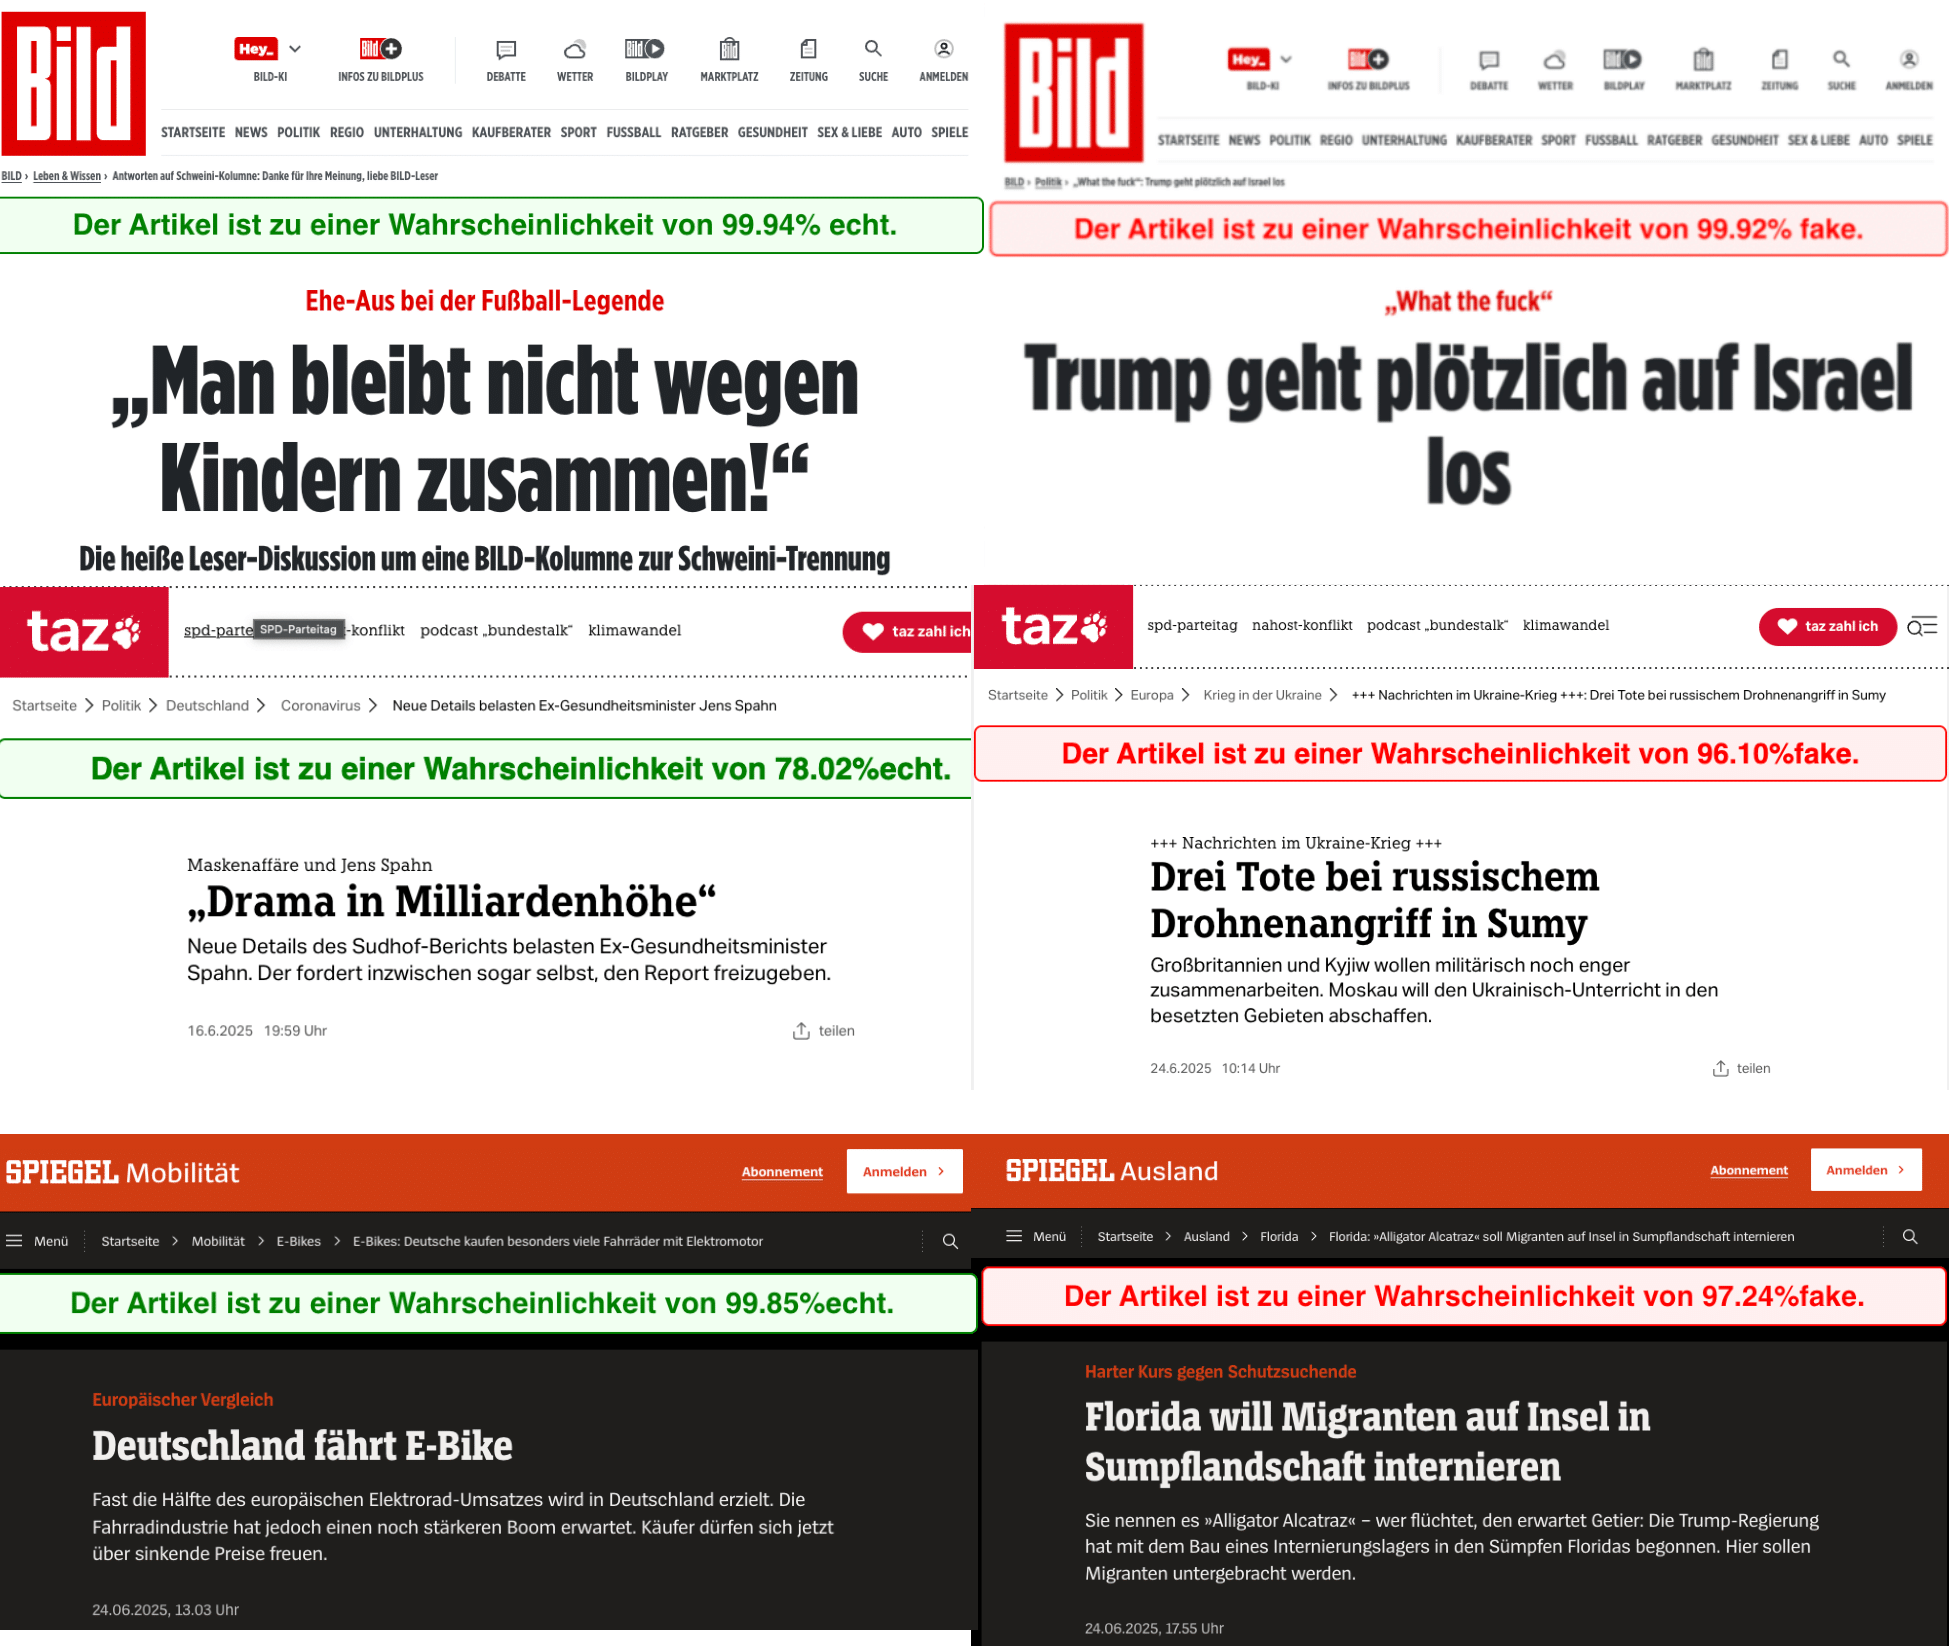
\includegraphics[width=\linewidth]{static/screenshots_anwendung.png}
        \caption{\label{fig:screenshot_anwendung} Screenshots der Anwendung auf den verschiedenen Nachrichtenportalen - faktisch sind alle Artikel korrekt}
    \end{center}
\end{figure}
\chapter{Diskussion}
\label{chap:diskussion}
\chapter{Fazit und Ausblick}
\label{chap:fazit_und_ausblick}
% Add additional chapters here


%\bibliographystyle{plain}
\bibliographystyle{dinat}
\bibliography{literature}

% Appendix
\appendix
% !TEX root = ../thesis.tex
% appendix example chapter
% @author Thomas Lehmann
%

\chapter{Anhang}

\section{Verwendete Hilfsmittel}
In der Tabelle \ref{tab:tooling} sind die im Rahmen der Bearbeitung des Themas der \IthesisKindDE~verwendeten Werkzeuge und Hilfsmittel aufgelistet.

\begin{table}[h!]
\caption{Verwendete Hilfsmittel und Werkzeuge}
\begin{tabular}{|l|l|}
\hline 
\rowcolor{lightgray} Tool & Verwendung \\
\hline
\LaTeX & Textsatz- und Layout-Werkzeug verwendet zur Erstellung dieses Dokuments \\
\hline
 & \\
\hline
\end{tabular}
\label{tab:tooling}
\end{table}



\IGlossary

\Istatement

\end{document}
